\documentclass[twoside]{styles/uocthesis}

\usepackage{subcaption}
\captionsetup{compatibility=false}

\usepackage[toc,page]{appendix}

\usepackage[pdftex]{graphicx} %Loading the package
\graphicspath{{figures/}} %Setting the 
\usepackage{mathtools}
\usepackage{bm}
\usepackage[flushleft]{threeparttable}

\usepackage{adjustbox}
\usepackage[acronym]{glossaries}
\usepackage{booktabs}
\usepackage{styles/gnuplot-lua-tikz}
\usepackage{tikz}
\usepackage{amsmath}
\usepackage{enumitem}

\usepackage{csquotes}

\usepackage{todonotes}
\usepackage{float}
\usepackage{makecell}
\usepackage{multirow}

\usepackage{url}
\usepackage[all]{nowidow}
 


\tolerance=9000
\pretolerance=5000
\emergencystretch=0pt

\righthyphenmin=4
\lefthyphenmin=4

\setlist{parsep=0pt,listparindent=\parindent}


\Title{Verification Based Annotation for Visual Recognition}
\Author{Oliver Batchelor}
\Year{2019}

\Supervisor{Prof. Richard Green}
\Department{Department of Computer Science}

\makeglossaries




\begin{document}

\prelimpages


\titlepage


\abstract{%

Applying deep learning to new domains usually implies a data collection and annotation problem. While several large datasets exist and provide a great deal of utility, there is a need to apply deep learning to new domains more easily, and to more easily experiment without the burden of spending a large amount of time upfront to annotate data. This thesis explores some the ideas and tools needed for rapid prototyping with image data and convolutional neural networks. 
I have focused on visual recognition methods (initially image segmentation, and then object detection) where I've developed ``Human in the loop'' collaborative human--machine annotation methods where both machine and human annotator can be involved at almost every step of the process. 

% One key mechanic is that of verification based annotation, which works if verifying annotation is faster than manually inputting those validations from scratch. Another aspect is example selection, where the machine attempts to find the most informative examples for annotation at each step. Finding mistakes in annotation is usually performed by human verification, I attempt to see how that might 


}

\tableofcontents



\printglossaries

\newacronym{VBA}{VBA}{Verification Based Annotation}
\newacronym{FCN}{FCN}{Fully Convolutional Network}
\newacronym{FPN}{FPN}{Feature Pyramid Network}


\newacronym{FP}{FP}{False Positive}
\newacronym{FN}{FN}{False Negative}

\newacronym{TN}{TN}{True Negative}
\newacronym{TP}{TP}{True Positive}

\newacronym{IID}{IID}{Independent and Identically Distributed}

\newacronym{IOU}{IoU}{Intersection over Union}
\newacronym{VOC}{VOC}{Visual Object Classes}
\newacronym{mIOU}{mIOU}{mean Intersection Over Union}

\newacronym{mAP}{mAP}{mean Average Precision}
\newacronym{AP}{AP}{Average Precision}


\newacronym{CRF}{CRF}{Conditional Random Field}

\newacronym{RELU}{ReLU}{Rectified Linear Unit}
\newacronym{PRELU}{PReLU}{Parameterised Rectified Linear Unit}
\newacronym{DECAF}{DeCAF}{Deep Convolutional Activation Feature}

\newacronym{FPN}{FPN}{Feature Pyramid Network}


\newacronym{NLL}{NLL}{Negative Loss Likelihood}
\newacronym{BCE}{BCE}{Binary Cross Entropy}
\newacronym{CE}{CE}{Cross Entropy}
 
\newacronym{COCO}{COCO}{Microsoft Common Objects in Context}
\newacronym{ILSVRC}{ILSVRC}{ImageNet Large Scale Visual Recognition Challenge}

\newacronym{NN}{NN}{Neural Network}
\newacronym{DNN}{DNN}{Deep Neural Network}

\newacronym{CNN}{CNN}{Convolutional Neural Network}
\newacronym{MCDNN}{MCDNN}{Multi-Column Deep Neural Network}

\newacronym{SSD}{SSD}{Single Shot Detector}
\newacronym{RCNN}{R-CNN}{Region CNN}

\newacronym{NMS}{NMS}{Non Maxima Suppression}


\newacronym{SIFT}{SIFT}{Scale Invariant Feature Transform}
\newacronym{SURF}{SURF}{Speeded Up Robust Features}

\newacronym{ALOI}{ALOI}{Amsterdam Library of Images}
\newacronym{MSR}{MSR}{Microsoft Research}
\newacronym{AMT}{AMT}{Amazon Mechanical Turk}

\newacronym{BOW}{BoW}{Bag of Words}
\newacronym{BOVW}{BoVW}{Bag of Visual Words}

\newacronym{ANN}{ANN}{Approximate Nearest Neighbour}
\newacronym{SGD}{SGD}{Stochastic Gradient Descent}
\newacronym{ASGD}{ASGD}{Asynchronous Stochastic Gradient Descent}
\newacronym{LOO}{LOO}{Leave One Out}

\newacronym{NCA}{NCA}{Neighbourhood Components Analysis}
\newacronym{MEGM}{MEGM}{Mean square Error's Gradient Minimisation}

\newacronym{KNN}{kNN}{k-Nearest Neighbour}

\newacronym{MSE}{MSE}{Mean Squared Error}
\newacronym{LMNN}{LMNN}{Large Margin Nearest Neighbour}
\newacronym{NCM}{NCM}{Nearest Class Mean}

\newacronym{SVM}{SVM}{Support Vector Machine}

\newacronym{PCA}{PCA}{Principle Components Analysis}
\newacronym{DRLIM}{DrLIM}{Dimensionality Reduction by Learning an Invariant Mapping}
\newacronym{SGDR}{SGDR}{Stochastic Gradient Descent with Restarts}


\newacronym{GPU}{GPU}{Graphics Processing Unit} 
\newacronym{CPU}{CPU}{Central Processing Unit}

\newacronym{API}{API}{Application Programming Interface} 

\newacronym{GHC}{GHC}{Glasgow Haskell Compiler}
\newacronym{GHCJS}{GHCJS}{GHC for JavaScript}

\newacronym{HTML}{HTML}{HyperText Markup Language}
\newacronym{SVG}{SVG}{Scaleable Vector Graphics}

\newacronym{HTTP}{HTTP}{HyperText Transfer Protocol}
\newacronym{JSON}{JSON}{JavaScript Object Notation}

\newacronym{ID}{ID}{Index of Difficulty}
\newacronym{AWS}{AWS}{Amazon Web Services}

\newacronym{CAT}{CAT}{Cumulative Annotation Time}
\newacronym{ROV}{ROV}{Remotely Operated Vehicle}


\acknowledgments{%
I will like to thank all the hedgehogs, without there help this
thesis would not be a reality.}

\textpages 

% \setcounter{chapter}{0}
% 


\chapter{Introduction}

In this chapter I discuss firstly the broader context of research which relates to interactive annotation as it applies to this work. I discuss the topics in general, but also focus on applications to image processing with \gls{CNN}s. In section \ref{sec:closest} I then spend some time to compare and contrast the most specific research efforts most similar to this work.

\section{Research goals and contributions}

The central thesis to this dissertation is that annotation of data can be performed as a collaboration between human and machine learning algorithm. This by itself is not new idea, and is known as 'human in the loop' machine learning. Given the wide variety of visual recognition task, and thus different kinds of work-flow for annotation - I look to provide the best set of tools to empower the human annotator.

Specifically I look at two aspects where a machine learning algorithm assists a human annotator. The first and main focus is verification based annotation where a human annotator annotates a dataset by validating machine generated predictions.

The second focus is organising data and example selection - allowing an annotator to sort images, then find the best images to annotate first and then find mistakes or inconsistencies. 

A large part of crowd sourced annotation is having cross verification. I look at how a machine learning algorithm can help verify a dataset instead, to weed out errors by finding and showing inconsistencies in the provided data.

I explore the topic in a modern scenario using \gls{CNN}s, and aim to show the approach is very practical for annotation of a range of visual recognition datasets. I do this through developing tools for human in the loop image annotation and performing a series of experiments to answer questions and validate my ideas. I also demonstrate it's use on a series of real world image annotation tasks.


\subsection {Thesis summary and contributions}

This thesis is split into roughly two parts, firstly works which stand alone - and is presented first, chapter \ref{chap:focus} where I look at the effect of cropping and resolution on image classification, and \ref{chap:metric} where I experiment with a new method of metric learning for instance recognition, a kind of n-way siamese network. 

The rest of the thesis from \ref{chap:bootstrap} onward is devoted to the central topic of the thesis, namely human in the loop machine learning. In chapter \ref{chap:bootstrap} I discuss verification based annotation for segmentation data where images are annotated by drawing masks over areas of interest. I explore several angles for assisted image annotation, and conclude that the verification based bootstrapping process to be the most promising. Contrary to popular belief that \gls{CNN}s require much data and much training time. I demonstrate the opposite that using few images, and also very little training time a \gls{CNN} can be trained to a level to provide very real assistance to a human annotator. 

In chapters \ref{chap:object_detection} I experiment with a state of the art object detection \gls{CNN} model and look at properties useful for human in the loop annotation. I look at practical aspects of training, including training one class at a time, cyclical learning rates and experiment on several small scale (but real world) datasets. 


Chapter \ref{chap:object_detection} is devoted to the design and implementation of a human in the loop annotation system 

I also look at example selection methods, where I look at how an annotation tool can facilitate annotation workflows for different kinds of image data. I briefly explore methods of effectively reviewing existing annotations for consistency, and how unlabelled data can be more effectively sorted and processed.

I demonstrate the utility of the tool by annotating several new object detection datasets (and validate it on a few older ones),  and collaborate with others who use it to annotate datasets.



\subsection {Rapid prototyping}

Not only is it necessary to collect and annotate data - one of the primary questions asked when considering the use of machine learning is 'How many examples are necessary?'. To which the usual answer is to by experimental validation where part of the data is held back and used to test the effectiveness of training on the other part. In this work I don't change 



\section {Thesis structure}


\section {Background}

Crowd sourcing. Human in the loop. verification based annotation.

Uncertainty, active learning.

Related ideas are are those which aim to make more effective use of data available. This includes methods to enrich existing data such as semi-supervised learning and hard example mining \cite{Jin2018, Yu2018, Canevet2014}, as well as those aiming to accelerate the learning process by sampling the data in the right order, including curriculum learning and self paced learning.

Transfer learning attempts to accelerate learning on a new domain by using knowledge gained through learning on another (usually much larger and more general) domain. It has been shown that (especially for images with \gls{CNN}s) that models trained on these datasets can be re--purposed in a variety of useful ways.


\subsection {Crowd Sourcing}

The most common approach to annotating a dataset is crowd sourcing. Crowd sourcing enlists the services of many in order to provide 

Most large scale datasets are created with some form of crowd sourcing, notable examples ImageNet classification \cite{JiaDeng2009}, Coco object detection \cite{Lin2014} or Cityscapes street scenes \cite{Cordts2016} are all created with crowd sourcing. 

In order to get a lot of people to contribute there exist methods such as gamification, where the task is turned into a fun game  e.g. a game Quick Draw \cite{Ha2017}, or presenting the task as proof of humanness \cite{Goodfellow2013a}. Citizen science uses volunteers to perform tasks, for example to count penguins, identify species or identify planets \cite{Simpson2014, Masters2016}. Often the feeling of contributing to something meaningful, or the novelty of having your name as a contributor is enough to bring people to be involved.

If there exists no easy way to bring people to help for free, then use of labour markets such as \gls{AMT} are an option. These markets enable an employer to pay for mechanical tasks involving human intelligence. Many large scale datasets such as ImageNet \cite{Russakovsky2015} are built with \gls{AMT}. 


\subsection{Human in the loop}

Human in the loop machine learning encompasses a range of machine learning techniques which utilise human input in effective ways. Either by providing assistance to a human annotator with verification based annotation, or by having the annotator assist a learner which tries to make the most out of annotator time, such as active learning.

Machine learning datasets often contain a lot of so called ``easy'' examples. These examples often dominate both the annotation process where human time is spent needlessly annotating similar easy examples, and in the learning process where the learning algorithm spends much of it's computation time on examples which are already handled well. 


\subsection{Verification based annotation}

\begin{figure}[h]
  \centering
  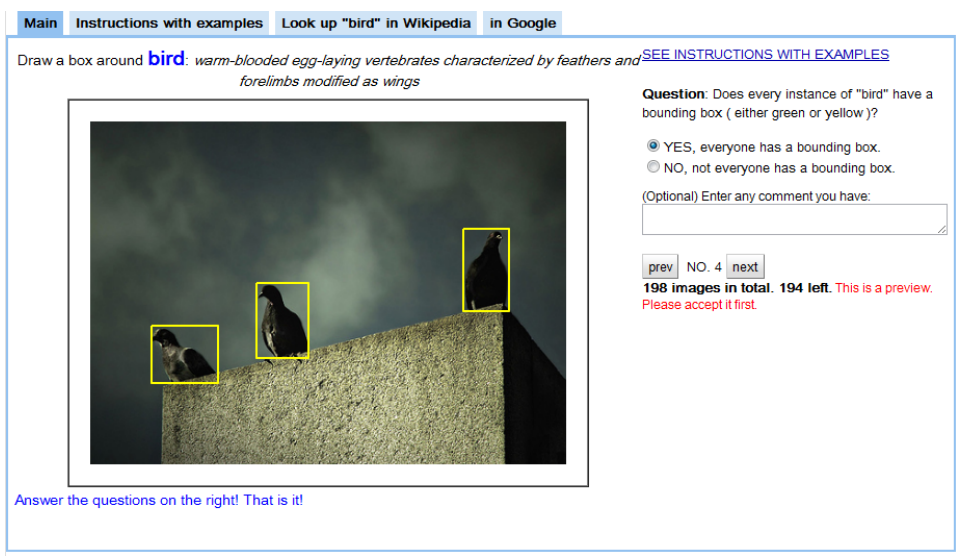
\includegraphics[width=0.9\linewidth]{introduction/crowdsourcing_annotation.jpg}
  \caption{Crowd sourcing image verification task in \cite{Su2012a}}  
  \label{fig:captcha}
\end{figure}

I coin the term verification based annotation, where machine annotations are checked and verified by a human annotator. Although the idea has played a central role in many previous works, it is not given an easily recognisable term to distinguish it for example from other kinds of Human in the Loop machine learning such as Active Learning (and is often put in the same basket). A selection of verification based methods, many of them discussed in detail below \cite{Yao2012, McNeill2011, Adhikaria2018, Castrejon2017, Papadopoulos2016, Russakovsky2015a}. 

Verification also plays a large part in ensuring consistency even between human annotators in crowd sourcing efforts, where the annotations of any one user cannot be fully trusted - users are tasked with cross verifying each others' annotations in many of these efforts, an example of a crowd sourcing task for annotating boxes on Image-net \cite{Su2012a}.

Weaker algorithms (machine learning or otherwise) can be used to generate proposals which can be then validated by an annotator. An example of this is in \cite{McNeill2011} where computer vision algorithms generate proposed counts of a penguin colony, and a human operator marks false negatives and false positives.

Human verification is fast, in \cite{Papadopoulos2016} reports a yes/no verification as taking 1.6 seconds on average. For a full annotation of an \gls{ILSVRC} image \cite {Su2012a} the time to draw a bounding box is reported at 26 seconds (42 seconds after quality control), but \cite{Papadopoulos2017} reports only 7 seconds per box using a more effective input method involving clicking extremities of objects rather than selecting corners. 

\begin{figure}[h]
  \centering
  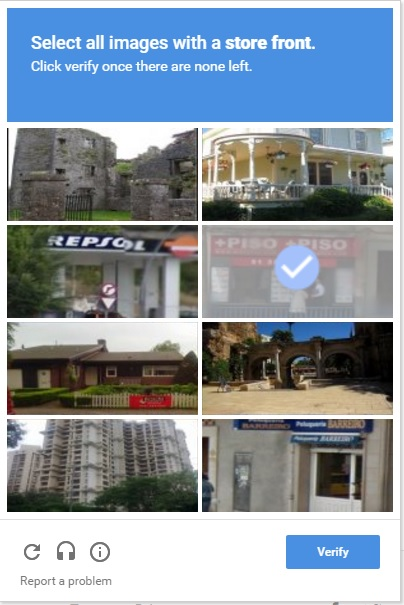
\includegraphics[width=0.9\linewidth]{introduction/recaptcha.jpeg}
  \caption{reCAPTCHA dialog showing multi-image verification task}  
  \label{fig:captcha}
\end{figure}

The human ability to verify many examples at once has often be used, for example in recent tasks presented by the well known reCAPTCHA \cite{von2008recaptcha} a grid of images is presented asking a user to select all instances containing a particular object or type of scene, this is shown in figure \ref{fig:captcha}. To my knowledge there is no study confirming if visually validating multiple occurrences together is more efficient than validating single occurrences, but given it's wide use it seems that is likely the case. 

Previous studies on verification based annotation such as \cite{Papadopoulos2016} focuses on localisation for the ImageNet dataset which features typically few large object instances per image (due to it's origins as an image classification dataset), with smaller instances often in the background. On domains with many smaller objects such as in biological studies of animals, verifying many instances at once should be much more effective. 


\subsection{Example selection and active Learning}

One prominent ``human in the loop'' method is active learning. Active learning revolves around picking the best set of examples for a human to annotate making most effective use of their time. Picking the best examples is often based around an uncertainty measure, where examples which a model is most uncertain about would often be the hard cases which are most useful for learning. 
 
While a \gls{CNN} used for classification provides some measure of uncertainty in it's output by way of it's softmax outputs, but this is usually not recommended and deemed unreliable. In \cite{Guo2017} it is shown that modern neural network architectures often systematically over estimate confidence, 

\gls{CNN}s with accurate uncertainty measures are much in their infancy, especially for more complex tasks such as object detection. However recent research gone into more effectively quantifying uncertainty in \gls{CNN}s with tools such as Bayesian \gls{CNN}s \cite{Gal2017} and other methods of estimating uncertainty have arisen such as ensemble variation \cite{Beluch2018} or minibatch variation \cite{Chang2017}. 

Specific to object detection one recent approach is to measure the stability of predicted boxes when noise is added to inputs \cite{Kao2018}. Another idea is to measure consistency between bounding box proposals \cite{Kao2018, Brust2018, Le2018}. Current state of the art object detectors such as \gls{SSD} \cite{Liu2016a}, or \gls{RCNN} \cite{Wang2011a} produce a multitude of box proposals - as such the variation can be measured.

Another measure used in active learning is expected change. An example of this is \cite{Vondrick2011} for video annotation, in which frames are selected for annotation which cause large expected change in the object track. Another example is \cite{Xu2017} where the expected change in an image's segmentation is used for the purpose of selecting which superpixels. 

Another related but distinct idea is making the best use of the examples available and in the best order. Curriculum learning and self paced learning \cite{Kumar2010} are research efforts devoted to this goal. Curriculum learning aims to learn from the most informative examples of a dataset in order to learn faster and more reliably, (a recent example is \cite{Katharopoulos2018}) self paced learning also attempts to have the learning algorithm also determine which examples are hard and easy as it progresses.


\subsection{Semi-supervised learning}

Semi-supervised methods are another active research area which aims to make use of more minimal labelling - either incomplete labelling or weak labelling. An example is in upgrading datasets with only category labels to datasets with localisation, one method involves using the internal activity of a \gls{CNN} to infer location of objects in an image \cite{Sivic2015}.

Semi-supervised ideas like hard example mining \cite{Loshchilov, } is commonplace in object detection. Negative examples are not explicitly annotated but found when false positives occur during training.

Properties such as temporal consistency can also be used to infer labels which are not explicitly annotated, if an annotated object exists on one frame in a video then it probably exists in adjacent frames, too.


\subsection{Interactive machine learning}

Many human in the loop processes (those which use human refinement to train a learner) are technically a form of interactive machine learning, but more specifically interactive machine learning uses human inputs to make predictions or modify it's behaviour directly.

Interactive machine learning is often used for segmentation where it takes considerable effort to input a segmentation mask, much more than to draw a bounding box for example. Object selection for example the GrabCut algorithm \cite{Rother} can be used to find object masks with approximate user input, such as scribbles or bounding box selection. Such a tool can be used iteratively to create, then refine an annotation with the annotator observing the output and making changes to the inputs.  LabelMe \cite{Russell2007} interface provides a scribble based object mask creation tool in this mould. 

More recently, the same ideas have been applied using \gls{CNN}s where a model can be trained to predict an object mask based on simulated user input, for example clicks \cite{Xu2016b, Boroujerdi2017}, bounding boxes \cite {Xu2017} or extreme points \cite{Maninis2017}. Human input can also be used to refine an output for example in medical segmentation \cite{Wang2017}, or for image colourisation \cite{Zhang} where it's primary purpose is to provide a more intuitive editing tool.

A contrasting interactive approach is to have a model provide outputs designed to be easily editable, such as PolygonRNN \cite{Castrejon2017} which provides automatic object selection by bounding box, but provides outputs as a polygon rather than as a mask. The benefit of this approach is that a polygon can be edited more precisely and fed back into training directly.




\subsection {Transfer learning}

Transfer learning is the idea of taking knowledge gained from a base task, and applying it to another. The most prominent and widespread use of transfer learning is perhaps the use of fine tuning or feature extraction.  Where models trained on classification tasks (typically ImageNet \cite{JiaDeng2009}) are re-purposed for usually much smaller scale tasks in different ways. 

\gls{DECAF} \cite{Donahue2014} showed features extracted from the hidden layers of a \gls{CNN} were directly transferable to achieve the then state of the art on a number of image tasks, including classification and as a much stronger replacement for the hand crafted \gls{SURF} descriptor \cite{bay2006surf}.  Specifically they used AlexNet  \cite{Krizhevsky2012} trained on ImageNet \cite{JiaDeng2009}.

In \cite{Yosinski} it is shown that the transfer-ability of features depends on the distance between the base task to the target task, and that using a pre--trained network can even improve generalisation after fine tuning (as compared to training from scratch).

Fine tuning retrains a network for a new task, typically using a lower (or zero) learning rate for some parts in order to preserve the learned 

The use of pre-trained models is now commonplace in adapting \gls{CNN} to new domains, with repositories of state of the art models pre-trained on large datasets existing for most machine learning frameworks (for example the PyTorch \cite{Paszke2017} model zoo. 

It is becoming standard practice, models for other tasks - for example segmentation or object detection are usually based around a network (the so called backbone of a network) which has previously been trained on a classification task. Examples include the widely used \gls{FPN} network, \cite{Lin2017a} where a base network, for example a ResNet \cite{He} or a DenseNet \cite{Huang2016} backbone which operates from high resolution to low, is combined by a secondary path which operates from low resolution to high with shortcut connections between, combining a pattern seen before in the segmentation U--Net \cite{Ronneberger2015} architecture with pre-trained models.

The \gls{FPN} is now used as a base model in a variety of state of the art segmentation and object detection methods, and seems widely applicable to a variety of tasks by attaching different network ``heads'' specific to the task at hand (such as classification, regression etc.).




\section {Most similar projects to this work}
\label{sec:closest}

\subsection {Interactive Object Detection \cite{Yao2012}}
Interactive object detection \cite{Yao2012} describes a human in the loop interactive annotation system, where an incremental object detector (Hough forest) is trained as a user corrects annotations provided by the system. 

The user interface consists of the ability to delete incorrectly predicted instances (\gls{FP}) and to add new bounding boxes where the object detector failed to produce them (\gls{FN}). A user study was done and found that \gls{FN} were almost twice as expensive as \gls{FP} to correct. Though it is not mentioned the exact mechanism required from the user to implement these edits. It could be because the cost of drawing a box is faster than selecting one for deletion.


The work in this thesis has a similar focus in many aspects, notably using an object detection algorithm with a predict--refine--train loop. 

In contrast, an emphasis is placed on active learning and predicting the amount of time required for a user to correct the object predictions provided by the model, in this thesis the focus on enabling the user. 

Hough forests \cite{Gall2011} are used as an online learning method for the purposes of being fast to train and fast for inference. One disadvantage of hough forests is that when annotation mistakes are made then the decision trees which arise from those mistakes can not be reversed. 

In this thesis I focus on using \gls{CNN} based object detectors (particularly RetinaNet \cite{Lin2017} and \gls{FPN} \cite{Lin2017a}) for the same purpose, which benefit from recent developments in object detection and are in general much more capable object detectors. Compared to the hough forests described, training can be slower, but inference is much faster on a modern \gls{GPU} than the figures provided for the hough forest (13 seconds).



\subsection{Fluid Annotation \cite{Andriluka2018}}
\begin{figure}[h]
  \centering
  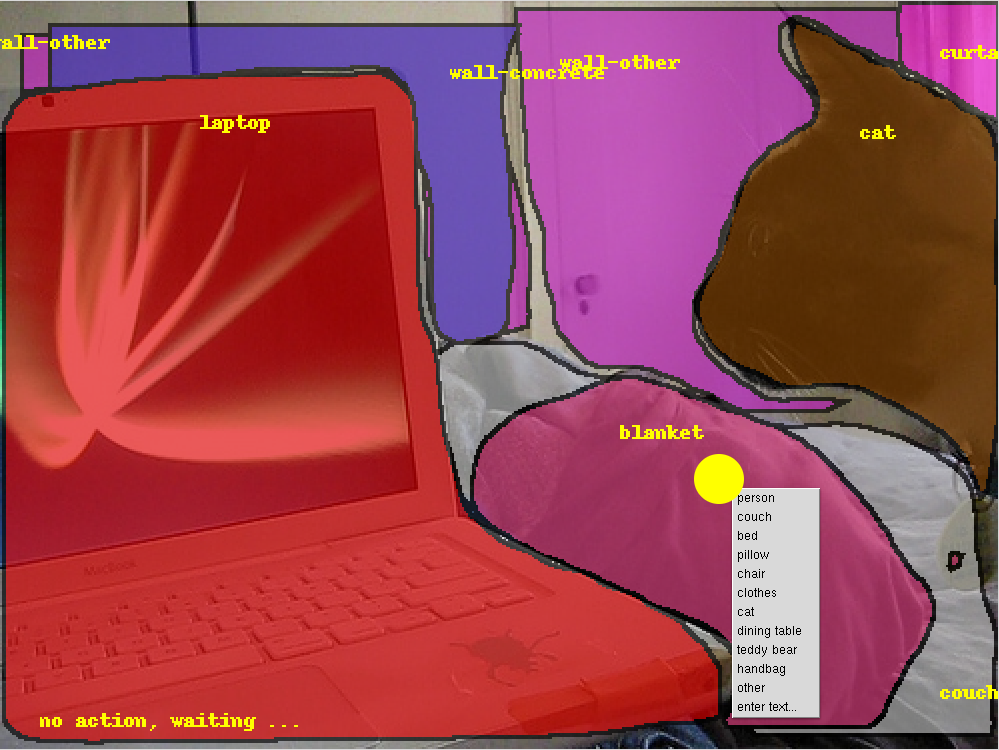
\includegraphics[width=0.9\linewidth]{introduction/fluid_annotation.png}
  \caption{User interface for Fluid Annotation \cite{Andriluka2018}}  
  \label{fig:fluid_annotation}
\end{figure}

Fluid annotation is an interactive human in the loop approach for instance segmentation. They point out three key points of their approach, the use of a strong neural network model, editing an entire image at once (as opposed to asking questions about each annotation one by one), and the approach to empower the annotator rather than employing clever methods to select examples (such as active learning). An example of the user interface is shown in figure \ref{fig:fluid_annotation}.

A key difference to my approaches is that I focus on annotating and experimentation with new domains, using transfer learning as a tool to enable online learning of the new domain. The strong neural network provides a power annotation aid, but limits you to annotate images in the same domain as that network (which is fine for many tasks).

\subsection{Faster Bounding Box Annotation for Object Detection in Indoor Scenes}
In \cite{Adhikaria2018}, an object detection dataset is annotated in two parts, first a small split is annotated and used to train an initial model, then the remaining data is annotated by having the human annotator validate and refine model predictions. My approach is similar in many ways, the difference is that I focus on iterating annotation and training immediately with an online learning approach.

\subsection {PolygonRNN}
Polygon-RNN \cite{Castrejon2017} uses a predict, refine, train approach in generating segmentation masks (as polygons), where a model is trained to segment generic objects then it can be fine tuned for a specific tasks where a user first provides a bounding box around an object, the model predicts a polygon and the refines the polygon and it is fed back for training.

\subsection {We Don't Need No Bounding Boxes}
In \cite{Papadopoulos2016}, a classification dataset is enriched with bounding box information. Instead of annotating a dataset from scratch - a model, and dataset are iteratively refined together by asking questions of a human annotator. They initially bootstrap a model using semi-supervised methods with per--image labels. A simple Yes/No questioning process is then used used to annotate a dataset by refining bounding boxes proposed by the model (and intelligently prune bounding box proposals by adjusting thresholds and overlap \gls{IOU}). They report the speedup to achieve nearly equivalent accuracy of $6\times$ to $9\times$.

In a similar vein \cite{Russakovsky2015a} uses a wider variety of interactions with the focus on obtaining a more complete set of annotations including those too difficult for current object detectors. The tasks include both question asking and manual annotation.

\subsection{Learning Intelligent Dialogs for Bounding Box Annotation}

Different kinds of annotation task can be approached in different ways, the focus of \cite{Konyushkova2017} is in choosing the appropriate interface for the given image. An example given is two images, one with many low scoring predictions - another with fewer high scoring predictions. To the first they have a user manually annotate boxes, to the second they have the user verify each detection separately.

This work also tackles the same issue in a different way in chapter \ref{chap:annotation}, I aim to provide a single user interface to cope with various situations by providing fine control over which object detections are displayed to the user and how 











% \setcounter{chapter}{1}
% 
\chapter{The Role of Focus in Object Instance Recognition}
\label{chap:focus}

This chapter was published in \cite{Batchelor2017} by a paper with the same name. I present a study on the effects of focus on object instance recognition (identifying instances of the same object or very similar object, for example a particular product) using a \gls{CNN}. The field of object detection is seen as a harder task than that of recognition, as the object must be localised as well as classified. In the field of face recognition, alignment is seen as a crucial step for the purpose of recognition - it is our hypothesis that focus and alignment is similarly important for object instance recognition. 

I perform some experiments to verify the effects of localisation, using datasets with bounding box annotations. I found that CNN classification on images cropped to bounding box regions is much more accurate than classification of whole images. Both magnification and centring of the object in question seem to also have a strong effect. Including context in the classification is only useful if it does not come at the expense of minifying (down scaling) the object to be classified.
 
I conclude that in order to produce a quality instance recognition using \gls{CNN}s for classification, it would be a big advantage to first localise and then focus on the region of interest. Future research will focus on how this localisation can be performed, for example using a model to first estimate a bounding box and rotation using regression, or using Spatial Transformer Networks which enable learning a joint classification and focus method.




\section{Introduction}

Object detection is described typically as a harder problem than object recognition, only because it requires not only classifying which object is present, also establishing where each object is located. I look at this from another angle. If the location of each object is first located, is it possible to identify what object is present? 

Convolutional Neural networks (\gls{CNN}s) \cite{LeCun1998} have become the tool of choice for image classification problems in recent years. Despite having been invented many years earlier it was the advent of \gls{GPU}s enabling larger datasets and larger networks which triggered its adoption, initially coming to prominence in \cite {Krizhevsky2012}.  I experiment with how focus influences the performance of a CNN model for the purpose of instance recognition. My interest is in instance recognition, although I can see that these ideas are not unique to instance recognition, but for object recognition and classification with \gls{CNN}s in general.

\gls{CNN}s are said \cite{Krizhevsky2012}, to have properties which make them invariant to translation, and they naturally learn redundancy to scale and rotation present in the training data. Is it necessary then, that \gls{CNN}s, must be focused and aligned on the exact area of interest? The role of focus and alignment can be seen most clearly in face recognition, where faces are aligned very precisely. Face recognition almost ubiquitously uses alignment as a pre-processing step, before passing images on to a model for recognition purposes even when the model is a deep CNN \cite{Taigman2014}.

It seems intuitive that focusing on the relevant part of an image should produce a better outcome, however also being aware that the context of an object is said to be important in recognition \cite{Oliva2007}. For example the background of water and sky gives a strong clue that an object is more likely to be a boat than a car. A cluttered background is seen as a problem in object recognition and detection, and it was noticed in an effort to compare image patches, that prioritising pixels in the centre of a patch \cite{Zagoruyko2015} increased performance. In this light, it is unclear if including context in image classification is always advantageous. 

I look at this in the context of object instance recognition with two datasets where objects have been localised with bounding boxes. I use two instance recognition datasets the Washington RGB-D dataset \cite{Lai2011} of object turntable sequences, and the INSTRE dataset \cite{Wang2015} containing photographs of objects captured by hand. In the case of the INSTRE dataset, most (but not all) objects are captured with backgrounds where context is not very predictive - for example a toy captured with a grassy background. The RGB-D dataset is captured in a controlled environment with a white turntable in the background in all images.

\gls{CNN}s are frequently used to learn alignment, for example bounding box regression is common in object detection \cite{Sermanet2013}. In face recognition facial features are commonly detected and used to align the face very closely with other face images, which is also typically performed using a CNN. For the generic task of object instance recognition I don't have the luxury of obvious landmarks for alignment, as they vary largely depending on the type of object, but I can consider more general alignment such as estimating bounding box(es) or using regression to estimate rotation as in \cite {Fischer2015}. 

Spatial transformers \cite{Jaderberg2015} are another option and enable a joint learning of a classifier and attention method (affine transformation) for \gls{CNN}s, with evidence they  house numbers in natural images \cite{Netzer2011} and bird species recognition \cite{Wah2011} In future I will evaluate these alignment methods for the purpose of object recognition as well as consider methods of capturing object images with bounds and orientation, however if identifying the correct focus is more difficult than recognition, there is little point.


\section{Method}

I use the same training method, and optimisation method throughout, except where mentioned and the parameters are as described in this section. 

\subsection {Learning}

I use standard \gls{SGD} with momentum set to $ 0.9 $. I set the learning rate to $ 10^{-2} $ and interpolate this rate across each epoch to a minimum of $ 10^{-4} $. I interpolate the learning rate using \gls{SGDR}  \cite{Loshchilov2016}, however I reduce the learning rate at each mini-batch instead of each epoch. I set our epochs to be relatively large accordingly, and restart SGD at the higher learning rate at the beginning of each epoch. 

Each training cycle was performed with epoch sizes of 65536, and 10 epochs were trained in all cases, after which the loss function plateaued. I use a mini-batch size of 64, and an image size of $64\times64$ (although this is varied for some experiments). I select images from each class randomly with uniform probability, as well as images from within each class with uniform probability.

\subsection {Network}

I use the same architecture CNN in each case, varying slightly for experiment two where I increase the pixel size of the input image (see below for details). I use a simple AlexNet \cite {Krizhevsky2012} style model, and details are given in table~\ref{fig:focus_network}. Other network architectures, such as the popular ResNet \cite{He2015} style were evaluated, and perform very similarly at the tasks presented here, but at the expense of taking longer to train.

Each convolution operation is padded, in order that inputs and outputs dimensions match (e.g $ 7\times7 $ convolutions have inputs zero padded by 3 pixel, and $3\times3$ convolutions have inputs zero padded by 1 pixel). It can be seen that each layer (ConvLayer) halves the input resolution after convolution, using max-pooling. For a non linearity I use the \gls{PRELU}. Batch Normalisation is used directly before all convolution layers and uses a running sum with momentum = 0.9.

Our classification method is the standard SoftMax method with the usual cross entropy loss function. Before the final linear layer I use a single dropout layer $ p = 0.5 $, which I have found prevents over-fitting even though it is said to be unnecessary to use both batch normalisation and dropout.  I use the Torch7 \cite{Collobert2011a} neural network library to implement this network and perform all experiments. 

\begin{table}[h]
  \centering
    \caption{Neural network structure }
\begin{tabular}{ l } 

\toprule

 ConvLayer(n) = PRelU $\rightarrow$ Batch Normalisation \\ 
 $\rightarrow$  Convolution $(3\times3, n \rightarrow n * 1.5)$ $\rightarrow$  Max Pooling $(2\times2)$ \\
\\
 LinearLayer(m, n)  = PRelU $\rightarrow$ Batch Normalisation \\  $\rightarrow$  Linear $(m \rightarrow n)$ \\
\toprule
  Network = Batch Normalisation $\rightarrow$
 Convolution $(7\times7, 3 \rightarrow 32)$ \\
 $\rightarrow$ Max Pooling $(2\times2)$   \\

  $\rightarrow$ ConvLayer (32) $\rightarrow$  ConvLayer (48) $\rightarrow$ ConvLayer (72) $\rightarrow$ ConvLayer (96)   \\
  
  
  $\rightarrow$ Flatten $(2\times2\times144 \rightarrow 576)$ $\rightarrow$ LinearLayer (576, 256) \\
  
  $\rightarrow$ Dropout(0.5) $\rightarrow$ LinearLayer (256, $\vert classes \vert$ )  $\rightarrow$  SoftMax($\vert classes \vert$) \\
  
    
       
\toprule
\end{tabular}

\label{fig:focus_network}
\end{table}




\subsection {Image Preparation and Pre-processing}


\begin{figure*}[t]
    \caption{Examples of data augmentation }
\centering
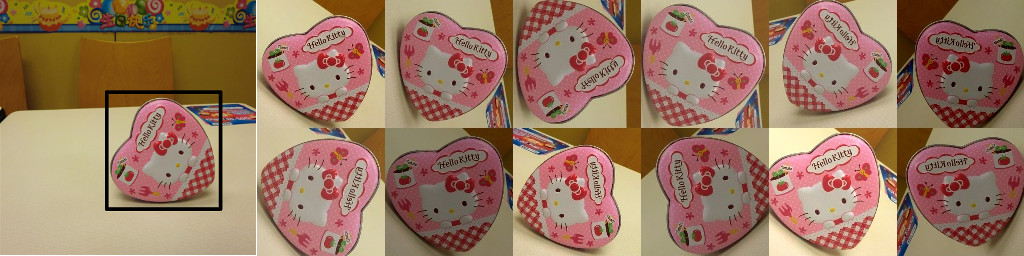
\includegraphics[width=1.0\textwidth]{focus/image_variations.jpg}
\label{fig:focus_variations}
\end{figure*}


In cropping an image to its object's bounding box, I use a uniform scaling - in order to ensure the entire object fits within this bounding box I fit a square around the bounding box in the cases where the bounding box is not square (I use square images as inputs to neural networks in this work).

I used data augmentation heavily to regularise the training in the form of random image transformations. Training images are randomly transformed using a set of parameters sampled from a normal distribution and shown in table~\ref{fig:focus_jitter}.  I use translations, rotation about the centre, scales (uniform and non uniform), and brightness and contrast adjustments. Testing images are re-sized and cropped in the same way (described below), but with no random transformations. An example of training data is given in figure~\ref{fig:focus_variations}.

\begin{table}[h]
  \centering
    \caption{Ranges of parameters used for image distortion }
    
  \begin{tabular}{ l  l }
    Parameter & Mean $ \pm $ Standard deviation \\
    \toprule
    scale (uniform) & $ 1 \pm 0.2 $  \\ 
    non uniform scale  & $ 1 \pm 0.2 $  \\ 
    rotation (degrees) & $ \pm 90 $ \\ 
    translation(x, y) (\% image size) & $ \pm 5 $ \\ 
    brightness (additive) & $ \pm 20 $ \\ 
    contrast (multiplicative) & $ 1 \pm 0.2 $ \\ 
    \bottomrule
  \end{tabular}
\label{fig:focus_jitter}
\end{table}


An affine transformation matrix $ (2 \times 3) $ is computed, firstly scaling the image to fit the bounding box region to match the network's input size, applying a set of random transformations as above, then cropping a rectangular region around the origin of the transformed image. I use OpenCV's \emph{warpAffine} function to perform this as a single step, avoiding artefacts from multiple image transformations (and also to avoid having to compute intermediate images with associated clipping issues).

\subsection{Datasets}

The RGB-D \cite{Lai2011} dataset contains turntable images with a fixed camera at 30 degrees, 45 degrees and 60 degrees of elevation. For evaluating instance recognition the 30 and 60 degree images are used for training, and the 45 degree images are used for testing. Bounding boxes are provided for each image (generated using depth information). The RGB-D dataset contains approximately 500 images (varying a little) for each instance, with 300 different object instances. I make no use of the depth images provided in the dataset.

The INSTRE \cite{Wang2015} aims to be a more diverse, better balanced dataset with more cluttered backgrounds than existing object instance recognition datasets. It improves on the RGB-D dataset in that the range of views are much more variety, both in the the types of object and the backgrounds (hand taken photos) compared with the turntable background. Bounding boxes are again provided. No standard test set is provided for the INSTRE dataset, so I take images of each object for testing, and use the remaining images for training at a ratio of $1:3$. The INSTRE dataset contains 200 classes of object, each with 100 images which have either been hand captured or picked. 

The INSTRE dataset contains unique challenges. A number of the objects are a little abstract, and include things like logos (e.g. one of the categories is KFC, which includes pictures of the building prominently showing the logo, as well as napkins containing the logo and pencil drawings). An example of a hard case is shown in figure~\ref{fig:focus_adidas}. Many categories feature objects rotated in numerous ways, with both landscape and portrait images, as well as many photos taken on angles with no alignment at all.

\section {Experiments}


\subsection {Experiment 1}

The first experiment compares the effect of focusing on the bounding box on classification accuracy. If there existed an oracle which could provide a bounding box estimate (or another model which could accurately give a bounding box estimate) - how much better is the network performance on cropped versus baseline (uncropped) images? I apply this cropping equally on test and training images.

For the RGB-D dataset, which for many of the objects only occupy a tiny space of the full image, I crop the inner centre to 40 percent of the image for the uncropped baseline. Otherwise, after scaling the original image to $ 64 \times 64 $ the smaller objects occupy only a few pixels, with the turntable and background being vastly bigger in scale. In order to see if the magnification from cropping to the bounding box was having an effect, I also ran the baseline at a higher resolution - but noticed little change in performance.


\begin{table}[h]
  \centering
    \caption{Cropped vs. uncropped images }
    
  \begin{tabular}{ l l l }
    
    Dataset & Image preparation & test set accuracy \\
    \toprule
    
    INSTRE & baseline &  65.3 \\
    INSTRE & bounds cropped & 89.0 \\
    
    RGB-D & centre cropped & 58.1 \\
    RGB-D & bounds cropped & 81.6 \\
    
    \bottomrule
  \end{tabular}
\label{fig:focus_crop}
\end{table}

The RGB-D results suggest over-fitting, with the training accuracy reaching almost 100 percent, yet generalising badly with the test set. The RGB-D images present a problem in that the test set (those images captured at 60 degrees elevation), is from a slightly different distribution from the training set (the images are captured at a constant level of elevation). Each image is also reasonably redundant due to being part of a video sequence. A potential solution to this is using a higher level of randomised non uniform scaling when training. The INSTRE images on the other hand have no systematic difference between training and test images and also cover a much greater intra-object variation but do not show the same kind of over-fitting.

It is clear that focusing on the bounding box has a large impact on the performance of the classification, with both RGB-D and INSTRE classification improved when trained and tested on images cropped to the bounding box. Given this is the case, I seek to discover exactly why. Which property is it that enables effective classification using this kind of CNN model? Is it the magnification of the object after cropping an image to the bounding box, or removing the distracting background? (It is clear the object is much larger in pixels after the resulting image is scaled to match the CNN input size). Alternatively, is it the centring of the object, suggesting the translation invariance of the CNN is not as general as is widely assumed?


\subsection {Experiment 2}

\begin{figure*}[t]
    \caption{Examples of cropping for context}
\centering
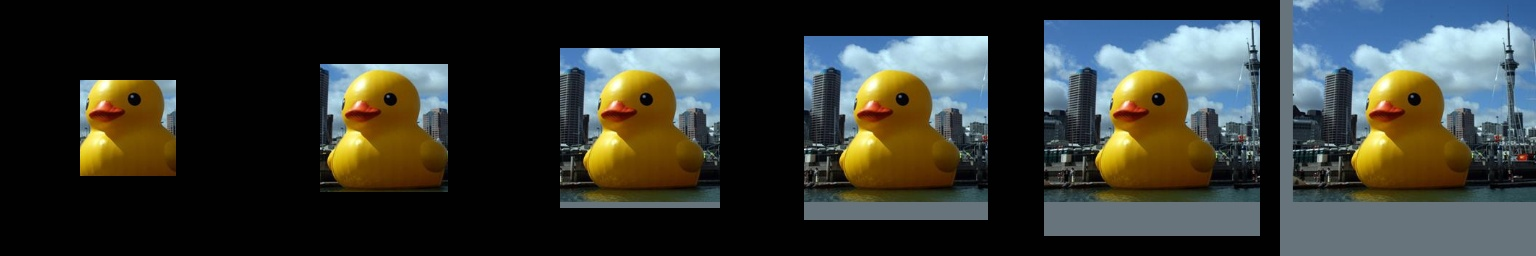
\includegraphics[width=1.0\textwidth]{focus/enlarge.jpg}
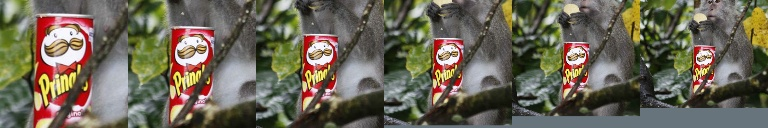
\includegraphics[width=1.0\textwidth]{focus/shrink.jpg}
\label{fig:focus_context}
\end{figure*}




\begin{figure}[h]
    \caption{Context in image classification vs. test set accuracy}
\centering
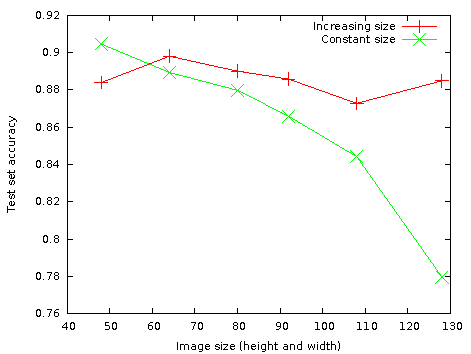
\includegraphics{focus/graph.pdf}
\label{fig:focus_exp2}
\end{figure}

For the second experiment I explore how including context changes the performance. I do this in two ways. Firstly by fixing the pixel size of our object and including more context by using a larger input image to the model. Secondly by fixing the size of the input to the network and including the same context, where the object is scaled down to accommodate.

In the first case I scale the object bounding box to $ 64 \times 64 $ and set this as the base scale, each larger size includes proportionally more context where the object remains a constant size in pixels. In the second case I use a fixed image size of $ 64 \times 64 $, using the same image context for each size as the first case, causing the object to be  scaled to be relatively smaller. 

The architecture of the network is mostly unmodified (each image output within the hidden convolutional layers in the network is of a larger dimension). The number of parameters is constant for the convolutional layers, but the first fully connected layer contains a larger number of inputs to cope with the extra outputs from the convolutional part. The differences can be seen in table~\ref{fig:focus_sizes}.


\begin{table}[h]
  \centering
    \caption{Example output sizes for input dimensions }
\begin{tabular}{ l l l } 
 
 \toprule
 Input image size & Convolution outputs & Flattened size \\
 \toprule
 
 $ 48 \times 48 \times 3 \rightarrow $ & $ 1\times1\times144 \rightarrow $ & 144 \\
 $ 64 \times 64 \times 3 \rightarrow $ & $ 2\times2\times144 \rightarrow $ & 576 \\
 $ 108 \times 108 \times 3 \rightarrow $ & $ 3\times3\times144 \rightarrow $ & 1296 \\
 $ 128 \times 128 \times 3 \rightarrow $ & $ 4\times4\times144 \rightarrow $ & 2304 \\
 
\end{tabular}
\label{fig:focus_sizes}
\end{table}

I can see from the data shown in figure~\ref{fig:focus_exp2} that performance is relatively constant where the scale of the object is fixed. Adding context neither gives a performance boost nor hinders recognition (only takes longer to train). Where context is added at the expense of the object scale I can see that at the higher levels the test accuracy drops.


\subsection {Experiment 3}

Given the results from experiment~2, it seems that reducing the scale of the object (in pixel size) causes a degradation of the performance. Experiment~1 shows that the unmodified INSTRE images are still much more difficult to classify for a CNN. Experiment 2 normalises scales between objects (for example.e. the Statue of Liberty becomes the same size in terms of image pixels as a can of cola). For experiment 3 I use the bounding box to centre the object, but leave the scale unmodified.


\begin{table}[h]
  \centering
    \caption{Effect of input size and centring}
    
  \begin{tabular}{ l l l l }
    
    Dataset & Input size & Test set accuracy \\
    \toprule
    
    INSTRE &  $ 64 \times 64 $ & 65.3 \\
    INSTRE &  $ 128 \times 128 $  & 71.7 \\
    INSTRE &  $ 192 \times 192 $  & 76.0 \\
    
    \toprule
    INSTRE (centred) &  $ 64 \times 64 $ & 71.6 \\
    INSTRE (centred) &  $ 128 \times 128 $  & 80.6 \\
    INSTRE (centred) &  $ 192 \times 192 $  & 84.2 \\
    
    
    
    \bottomrule
  \end{tabular}
\label{fig:focus_input_size}
\end{table}



I can see from this experiment that both increasing magnification, as well as centring the object both give significant accuracy boosts, not to the same level as cropping to the bounding box, but close. Perhaps even larger magnification would be fruitful. 

The fact that centring the object makes such a difference is surprising, given the translation invariance of the CNN architecture, however it is not clear exactly how much a CNN is translation invariant (even though I can see that the filters used in a convolution step are clearly translation invariant - it is not obvious that the network as a whole possesses such properties). A recent study attempting to quantify this translation invariance \cite{EricKauderer-Abrams2016} suggests the architecture, and data augmentation are both important here. 


\subsection {Failure cases - discussion}


\begin{figure*}[t]
    \caption{Example of one hard case in the INSTRE dataset}
\centering
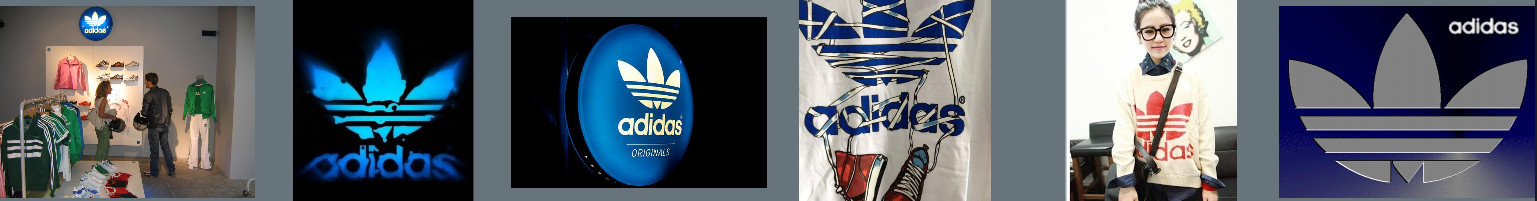
\includegraphics[width=1.0\textwidth]{focus/adidas.jpeg}
\label{fig:focus_adidas}
\end{figure*}



\begin{table}[h]
  \centering
    \caption{Worst categories in testing }
  \begin{tabular}{ l l }
  wangzai & 46.6 \\
  einstein bros & 46.6\\
  Manneken Pis & 45.4\\
  mastermind JAPAN & 45.1\\
  clapperboard & 43.2\\
  Che Guevara & 38.2\\
  coca cola & 33.3\\
  Paul Frank Julius & 32.4\\
  Kung Fu Panda & 24.0\\
  Adidas Originals & 17.2\\
    \bottomrule
  \end{tabular}
\label{fig:focus_failure}
\end{table}

It can be seen in figure~\ref{fig:focus_failure}, that many of the worst performing object classes were those which are somewhat abstract, for example logos which were stylistically the same logo but appeared visually quite different with different colours, materials and occurring in very different contexts. An example is shown in figure~\ref{fig:focus_adidas} for the ``Adidas Originals'' object.

\section{Conclusion}

I found that CNN classification on the cropped bounding box regions is much more accurate than classification of whole images. Both magnification and centring of the object in question seem to have a strong effect (which is somewhat surprising, given the translational invariance properties of CNN models). In the experiments I performed, including context in the input images was only useful if it does not come at the expense of minifying the object (reducing its pixel size) to be classified.

I conclude that in order to perform quality instance recognition using \gls{CNN}s for classification, it would be a strong advantage to first localise the region of interest, and then focus on the region of interest.  In future I will both further investigate why I see the results above, and at the same time peruse how focus methods can be used to improve instance recognition. The failure modes in unfocused image classification is also of interest for understanding in more depth our observations. For the INSTRE data set, the more abstract categories were among those which failed to generalise well, and RGB-D dataset simply over-fit badly.

I will explore bounding box regression as is used in many object detection methods, as well as rotation regression for the purposes of aligning input images to a canonical orientation. One difficulty with using regression is the requirement that your training data requires annotation, making its use in practice more expensive to obtain. Alternatives include using using external data, and using methods of semi-automated segmentation (for example using a green screen). Alternatively, the use of Spatial Transformer networks is interesting as it requires no such annotation, and jointly learns the focus method with the classifier.






% \setcounter{chapter}{2}
% 
\chapter{Object Recognition by Stochastic Metric Learning}
\label{chap:metric} 

Descriptors extracted from deep neural networks have been shown to be very discriminative. Networks such as those trained on the large, very general ImageNet dataset have been used to extract descriptors which can then be used robustly for a variety of image classification tasks. Such retrieval systems utilise feature locality, for example, Approximate Nearest Neighbour. The goal is to use such descriptors as part of a large scale object instance recognition and retrieval system. I propose using deep nonlinear metric learning on Convolutional Neural Networks to learn features with good locality. In particular, I worked with two related methods, \gls{NCA} and the related \gls{MEGM}.

I utilise a nonlinear form of \gls{MEGM} as an alternative to \gls{NCA} and propose some stochastic sampling methods to apply these batch learning methods to larger datasets with mini-batch \gls{SGD}. On a larger scale, I found the methods challenging to train, failing to converge or generalising poorly depending on the training method or parameters. This led to returning to a smaller dataset and examining the factors which lead to good generalisation with this form of training.
  
Surprisingly, on a small subset of the RGB-D dataset, stochastic sampling methods generalised much better with small batch sizes (they acted as a form of regularisation). When trained with larger batches, or as a full batch, the dataset was overfitted. Given the correct parameters, extracted descriptors performed well at the Nearest Neighbour task and exceeded the performance of those extracted by applying standard supervised training.

\section{Introduction}

Deep convolutional neural networks, in combination with modern \gls{GPU}s and large image datasets, have shown strong performance on image classification tasks \cite {Krizhevsky2012}, and have been applied to related problems such as object detection \cite{Sermanet2013}, image segmentation \cite{Masci2013} and image retrieval \cite{Razavian2014}.

\subsection {Descriptors from Deep Neural Networks}

Using descriptors, derived from the hidden layers of neural networks trained for classification, for the purpose of other learning tasks, is a relatively new idea. These descriptors have been shown to be robust even for quite unrelated tasks \cite{Donahue2014,Razavian2014}. The ImageNet dataset \cite{Krizhevsky2012} is a popular source for pre-training, and pre-trained models exist such as the OverFeat network \cite{Sermanet2013} or the DeCAF feature extractor \cite{Donahue2014}). 

A standard technique in training a \gls{CNN} is to augment the dataset by applying transformations, as more data typically gives better generalisation. In \cite{Dosovitskiy2013}, a \gls{CNN} was trained on single images which were warped in many different ways. Features obtained from the network were then used in popular classification benchmarks achieving good results. For many years local image descriptors such as \gls{SIFT} \cite{Lowe2004} have been used for matching and indexing images.  A recent comparison \cite{Fischer2014} (though perhaps not a fair one) showed that using a \gls{CNN} for matching tasks performed better than \gls{SIFT} by a margin similar to the improvement given by \gls{SIFT} to raw pixel data.


The final layer of a standard deep neural network, as used in supervised classification, consists of a set of linear classifiers, such as those descriptors that are suitable for classification using other linear classifiers, for example, \gls{SVM}s. Nearest Neighbor suffers from high dimensionality and noisy or irrelevant dimensions, so the descriptors produced by a CNN may not be suitable for comparison by distance. For that reason, I have looked towards metric learning to directly optimise the descriptors for Nearest Neighbor classification. 


\subsection {Deep Metric Learning}


Metric learning has often been used for object recognition and image classification \cite{Hadsell2006,Min2009} (and many others), and especially face recognition, for example \cite{Kostinger2012}. Although most efforts have often focused on Mahalanobis distance metric learning (a form of distance metric learning linear transformation), deep metric learning has had some attention \cite {Salakhutdinov2007a,Min2009,Weston2009,Min2010}. At the expense of a much larger computation cost, deep metric learning has been shown to perform much better than its linear counterparts. Gradients from metric learning are used to drive \gls{SGD} on a deep \gls{CNN}. 

Functions for metric learning often focus on pairs or triples, using siamese networks where parameters are shared between two or three branches of identical networks. This method generalises this to multiple examples at a time.

\subsection {Training}

Metric learning comes with its own set of challenges, and it has often been formulated as a batch training method because each example potentially interacts with every other example. In practice, descriptors from examples far apart do not interact with each other at all, so approximations can be made, as discussed later. High dimensional spaces from feature vectors can face issues, namely the ``curse of dimensionality''. In high dimensional spaces, evenly spaced points (descriptors) increase in the number of neighbours with increased dimension. 

The interaction between points decays with distance (for example, exponentially with \gls{NCA}). I can use approximations around the local neighbourhood of examples which can be used to create a \gls{SGD} training procedure. Using an approximation to the nearest $ k $, neighbours is an approach seen in \cite{Mensink2012,Zaidi2011} (among many). Clustering (amongst other sampling methods) is discussed in  \cite{Oneat2011} such as Farthest Point or Random Projection clustering, but the downside of such clustering is that it is hard to control the size of a batch. 

Many training methods focus on the interaction between pairs of (similar/dissimilar) examples or triples (example, more similar, less similar), for example, DrLIM \cite{Hadsell2006} where a spring analogy is used to create an attraction between similar pairs and repulsion between dissimilar pairs. The advantage of pairwise methods is that they can be used with the weaker labelling of similar/dissimilar (as opposed to category label).

\section {Deep Metric Learning}

A deep neural network (in this case a \gls{CNN}) is used to embed images into a lower dimensional space, creating descriptors which can be compared with their Euclidean distance (and classified with nearest neighbour) where the Euclidean distance of the raw pixels is both computationally expensive and not a good measure of the distance of the semantic similarity of image content. 

I examine non-linear versions of two methods, \gls{NCA} \cite{Goldberger2004} and the closely related but less well known \gls{MEGM} \cite {Zaidi2011}. \gls{NCA} optimises a continuous version of the \gls{LOO} performance, and it uses a softmax over weights which decay exponentially with distance. The \gls{NCA} score can be interpreted as the probability that a descriptor will pick another descriptor of the correct class as its nearest neighbour. 

The probability, $ p_{ij} $, of one descriptor selecting another descriptor as its neighbour, is defined as a softmax function over weights $W_ij$. The indexes $ i $ and $ j $ refer to input examples $x_i$ and $x_j$, and corresponding vector valued output of a \gls{CNN} $f(x_i)$ and $f(x_j)$ which are the descriptor vectors.

\begin{equation}
\label{eq:nca_prob_pair}
p_{ij} =  \frac {W_{ij}} {\sum_{k \neq i}{W_{ik}}}g
\end{equation}

Then the total probability, $ p_i $, of a point selecting any neighbour with another with its \emph{correct} class is defined as the sum of those neighbour probabilities $p_{ij}$ which have the same class:

\begin{equation}
\label{eq:nca_prob}
p_{i} =  \sum_{j:c_j = c_i}{p_{ij}}
\end{equation}

Where $ C_i $ is the class label of example $ i $. A Gaussian kernel is used for the weighting as \cite{Zaidi2011} do. 

\begin{equation}
 \label{eq:gaussian_kernel}
W_{ij} = exp(\frac{-\lVert f(x_i) - f(x_j) \rVert^2_2 }{2\sigma^2}), \space W_{ii} = 0
\end{equation}


The function to be maximised is the sum of the probabilities of all descriptors being correctly classified.

\begin{equation}
\label{eq:nca_loss}
\mathcal{E}_{nca} =  \sum_i {p_i}
\end{equation}

Where \gls{NCA} optimises directly on the probability $ p_{i} $ above, \gls{MEGM} instead computes for each class $ \hat{y_{ti}} $ as a prediction that a descriptor will take class $ t $, where the only difference is that $ c_j = t $ as opposed to $ c_j = c_i $:

\begin{equation}
\label{eq:megm_pred}
\hat{y_{ti}} = \frac{\sum_{j:c_j = t}W_{ij}}{\sum_{k \neq i}{W_{ik}}}
\end{equation}

The prediction $ \hat{y_{ti}} $ can then be compared with $ y_{ti} $ (1 where $ t = c_i $, 0 otherwise), and it then minimises the \gls{MSE} between prediction and true class label:

\begin{equation}
\label{eq:megm_loss}
\mathcal{E}_{megm} =  \sum_i\sum_t{(y_{ti} - \hat{y_{ti}})^2}
\end{equation}

Intuitively \gls{MEGM} can be seen to penalise the case where two classes compete for the same region,  more so than when one class competes against examples of many different classes, whereas \gls{NCA} would treat the two cases approximately equally. These loss functions can be used to drive gradient descent on a \gls{CNN} by standard back-propagation. The derivative for \gls{MEGM} is shown in the appendix, section~\ref{sec:appendix}.

The gradient is computed over the outputs of each mini-batch and apply back-propagation to find the derivative with respect to the weights of the network. It can be noted that the output and derivative for \gls{MEGM} is more expensive to compute because of the additional per class summation, so it would not be suitable with an extremely large number of classes. In practice, a large number of the terms can be factored out and pre-computed, as well as computing the difference summations in terms of matrix multiplication.

Note the parameter $ \sigma $ was not in the original \gls{NCA}, and is initialised to the average distance to the nearest neighbours of the initial descriptor output before training. It is used to prevent the weights initialising to zero when the distance between descriptors is large.


The parameter $\alpha $ controls the trade-off. When $ \alpha \mathcal{E}_{mse} > \mathcal{E}_{nca} $ the descriptors all collapse into the same point.


\section{SGD for metric learning}

The main proposal is in using mini-batch \gls{SGD}, and applying it to metric learning methods which have been designed as batch learning methods. Metric learning as shown above as a batch method, scales at $ O(n^2) $ for $ n $ examples. Given that the desire to apply these approaches to large datasets containing hundreds of thousands or millions of images, I am forced to consider approximations. The typical method for training a \gls{CNN} on large numbers of images is using \gls{SGD}, because it is fast, simple and scales to handle large datasets easily. 

The most obvious approximation is to truncate the influence to the nearest $ k $ neighbours as the weight exponentially decays with the square distance. It is hypothesised this would lead to the best approximation, however, there are many ways of truncating the neighbourhoods. This lends itself to clustering methods and is more complicated than the alternative, which is to sample batches randomly but uses a large enough batch to include several examples of each class.

I propose the following approaches for sampling batches for \gls{SGD}:

\begin{enumerate}
\item {\bf Random shuffled batches} \par
 Randomly shuffle the dataset and divide it up into batches of a fixed size, which is exactly how batches would normally be selected for supervised learning. Each batch contains (almost certainly) different numbers of examples from each class.
 \item {\bf Stratified random batches}  \par
 Pick batches by selecting a number of examples from each class, to ensure the same number of examples of each class are represented in each batch.   
 \item {\bf K-neighbourhoods around random points}  \par
 Before each training epoch, run the model forward through the training set to obtain descriptors for each example. Select N examples at random and pick the batch as the batch sized neighbourhood (in descriptor space) of each selected example.
\end {enumerate}


\subsection {Issues of Scale}

The parameter $ \sigma $ is optional in theory, as the scale can be factored into the final fully connected weight matrix (or previous layers).  I make use of $ \sigma $ for numerical stability upon initialisation, and during training the density of points adjusts itself to fit this parameter. It can also be observed that for different values of $ \sigma $, that the distance between descriptors adjusts themselves to fit the new parameter over a few iterations of training.


\subsection {Adding Mean Square Error}

I experimented with adding the square distance between members of the same class, as a means of adding some bias to the loss functions after suspecting that metric learning methods described above were overfitting, to force the output distribution to be more simple. 

\begin{equation}
\label{eqn:mse}
\mathcal{E}_{mse} = \sum_i{ \sum_{j:j_c = i_c}  \frac {{\lVert f(x_i) - f(x_j) \rVert^2_2}} {\sigma^2} }
\end{equation}

\begin{equation}
\label{eqn:mse_total}
\mathcal{E}_{total} =  \mathcal{E}_{nca} + \alpha \mathcal{E}_{mse}
\end{equation}


\subsection {kNN implementation}

I use a brute force \gls{KNN} algorithm written in CUDA \cite{Garcia2008} for the \gls{GPU}, computing the distance matrix using matrix multiplication followed by using an insertion sort to select the $ k $ neighbours of lowest distance. This approach is not scalable to large datasets, and smarter clustering algorithms will eventually need to be used; however, the time for evaluating \gls{KNN} on the datasets I experimented with, are still dominated by the cost of computing descriptors from examples. 


\section {CNN architecture}


\begin{figure}[ht]
\centering
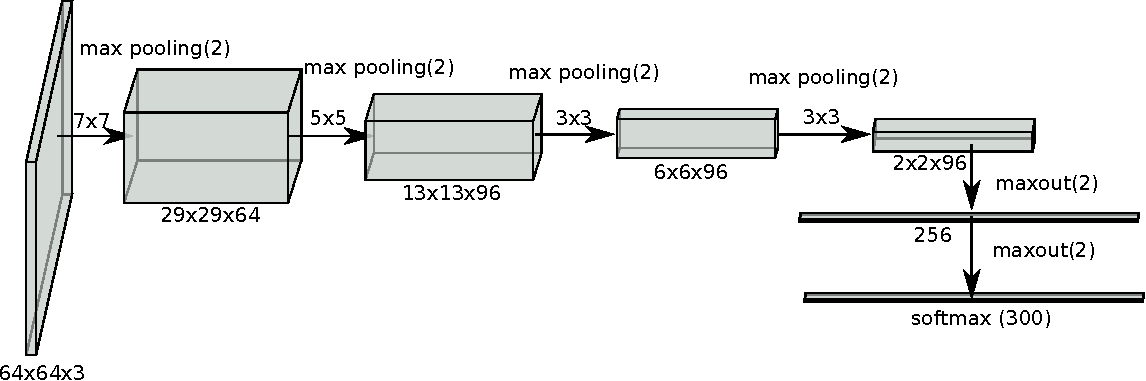
\includegraphics[width=1\textwidth]{metric_learning/convnet.pdf}
\caption{Convolutional network configuration used for $64\times64$ RGB images with supervised learning.}
\label{fig:metric_convnet}
\end{figure}

I used a simple convolutional neural network of six layers, with four layers of convolution and max-pooling using rectified linear activation functions, with two fully connected layers using Maxout \cite{Springenberg2013} units as an activation method, shown in Figure~\ref{fig:metric_convnet}. Dropout \cite{HintonDropout} with a rate of $ 0.5 $ is used when training on inputs to the two fully connected layers. For metric learning, the last linear layer and softmax are removed, leaving four convolutional layers and a single fully connected layer giving descriptors of size $ 256 $.

Dropout and Maxout have been shown to be beneficial in a supervised learning scenario for the purposes of regularisation. In the standard supervised training scenario, Dropout is of practical use because it (to some degree) prevents overfitting, and mostly does away with the need for early stopping. However, I found that it interfered with generalisation when used with metric learning approaches.

\subsection {Data augmentation}

\begin{figure}[h]
\centering
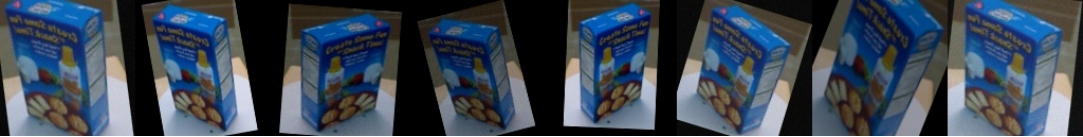
\includegraphics[width=1\textwidth]{metric_learning/augmentation.png}
\caption{Example of image distortions resulting from transformations of a single source image}
\label{fig:metric_augmentation}
\end{figure}


In all cases, I used randomised data augmentation of the test set by applying random distortions to ensure the network never saw exactly the same image twice, and to increase its tolerance to small changes in lighting, translation and rotation. The parameters of the data augmentation can be seen in Figure~\ref{fig:metric_permute}. Without the data augmentation, supervised training produces substantially worse generalisation than without, in both supervised and metric learning approaches. In all experiments, testing was performed on non-augmented images and trained with augmented images.

\begin{table*}
  \centering
    \caption{Ranges of parameters used for image augmentation }

  \begin{tabular}{ l  l }
    \toprule
    scale (uniform) & $ 1 \pm 0.2 $  \\ 
    squash  & $ 1 \pm 0.2 $  \\ 
    rotation (rads) & $ \pm \frac{\pi}{16} $ \\ 
    translation(x, y) (\% image size) & $ \pm 5 \% $ \\ 
    brightness (additive) & $ \pm 20 \% $ \\ 
    contrast (multiplicative) & $ 1 \pm 0.2 \% $ \\ 
    gaussian pixel noise & $ \sigma = 2 \pm 2 $  \\ 
    flip horizontal (probability) & $ 0.5 $ \\ 
    \bottomrule
  \end{tabular}
\label{fig:metric_permute}
\end{table*}

\subsection {Dataset}

\begin{figure}[h]
\centering
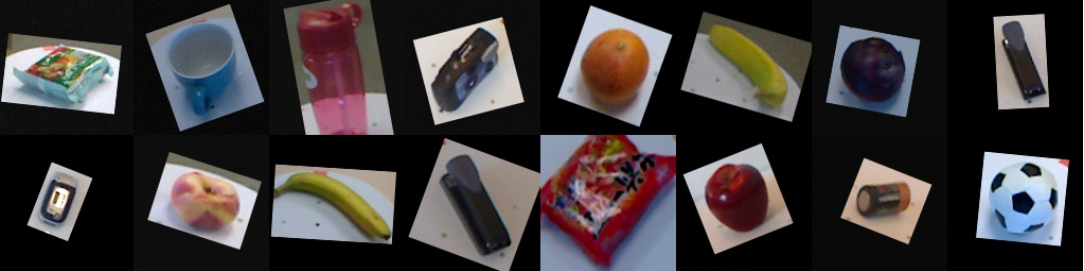
\includegraphics[width=1\textwidth]{metric_learning/objects.png}
\caption{Samples of images of different objects used in training}
\label{fig:metric_dataset}
\end{figure}

I experimented with the University of Washington RGB-D dataset primarily because it has a standard test set for instance recognition and a large number of published results. It contains 300 objects from 50 classes. Each object has three sequences of rotations at 30, 45 and 60 degrees elevation. Each rotation sequence contains approximately 150 images. For instance recognition, the sequence at 30 and 60 degrees are used for training, and the sequence at 45 degrees is used for testing. 

A cut-down version of the RGB-D dataset is used for a number of experiments, with 50 objects and 100 images of each object to train on, and 50 images per object to test. The images were randomly selected.

The resolution of $ 64\times64 $ on the RGB-D images is used, with the cropped version of the images. The procedure for resizing is to load all of the images in a sequence and if any image is at a higher resolution than $ 72\times72$, I resize the image to $ 72\times72 $. The same factor scales all other images in the sequence. The images are then augmented (see Figure~\ref{fig:metric_permute}) and finally centred (modulo translation) on a blank image at  $ 64\times64 $.


\section {Experiments}

In all cases (unless otherwise specified), I use a mini-batch size of 256, with standard \gls{SGD} learning rate set to $ 10^{-2} $ for supervised learning, and $ 10^{-5} $ for metric learning methods. I experimented with other learning rates for metric learning, and in some cases, a lower learning rate of $ 10^{-6} $ was used when the higher rate caused divergence.

I manually divided the training rate by a factor of 10 when the training set accuracy plateaus for supervised learning. Supervised learning methods greatly benefit from reducing the learning rate after time. However, there was no noticable benefit to the metric learning methods. I stopped metric learning methods at 70 epochs or earlier, if they were not converging. Overall, \gls{MEGM} gave similar, but slightly better test set accuracy than \gls{NCA}, and most experiments used \gls{MEGM} for consistency.


\subsection{Overall Comparison}

I compared the testing classification error between methods, and the final accuracy is reported as the test set classification accuracy average over the last 5 iterations. Test set accuracy is percentage accuracy. For metric learning, the class chosen is the most common class in $k = 5$ nearest neighbours.


\begin{table*}[ht]

\centering
  \caption{Summary of training methods}

  \begin{tabular}{  l l  l  l l l }
  
    \toprule
    method &  sampling & batch  & test accuracy &  train epochs \\  \hline
    \bf{Initialisation} & &  &  $ 64.0  $ & 0  &  \\  
    \hline
    
    \bf{Supervised} & & 256 &  $ 90.6  $ & 40  &  \\  
     & 5NN  &  &  $ 89.0  $ & 40 &  \\  
     \hline
    
    \bf{NCA} &  & batch &  $  71.2  $ &  50  & \\
     & random & 256 & $  94.0  $ & 70 & \\
    
    \hline
    
    \bf{MEGM} &  & batch  &  $  74.4  $ &  50  & \\
     & random & 128 &  $  95.0  $ &  70  & \\     
     &  & 256 & $  90.5  $ &  70 & \\  
     &  & 512 & $  81.4  $ &  70 & \\
    
    \hline
    \bf{MEGM} & stratified & 128 & $  {\bf 95.4 }  $ & 70 & \\  
    
     &  & 256 & $  94.6  $ & 70 & \\  
     &  & 512 & $  87.1  $ & 70 & \\  

     \hline
     
    \bf{MEGM} & neighbourhoods & 256 & $  80.4  $ & 70  & \\
    
    \hline
    
    \bf{MEGM + MSE} & stratified & 128 & $  {\bf 95.3 }  $ & 70  & \\

      \bottomrule
    
    \end{tabular}
\label{fig:metric_summary}
\end{table*}



I sought to compare the sampling approximation to the full batch (as opposed to mini-batch) method. As a batch method, \gls{SGD} is not the ideal training method. It was surprising to see that despite the loss function smoothly decreasing (as can be
seen in Figure~\ref{fig:metric_megm_test}), training failed to generalise well to the training set (Figure~\ref{fig:metric_megm_loss}).
I anticipated that the batch metric learning methods would work best as a batch
method or with larger batches (as closer approximations to the batch method).
It is seen that is not the case, and both the batch method and \gls{SGD} with the larger batch size (512) both failed to generalise well. The same pattern occurred for \gls{NCA}, as well as using the stratified sampling method. The reason for such overfitting is, I believe, that the two metric learning methods have not enough bias to force the network to learn something. \gls{NCA} allows highly complex and multi-modal distributions with many local minima, which provided the local neighbourhood structure fits, are not penalised by its loss function. Smaller batch sizes, however, act as a regularisation, forcing the descriptor outputs into a simpler form.



\begin{figure}[ht]
   \begin{tikzpicture}[gnuplot]
%% generated with GNUPLOT 4.6p1 (Lua 5.1; terminal rev. 99, script rev. 100)
%% Thu 31 Jul 2014 02:53:39 NZST
\gpsolidlines
\path (0.000,0.000) rectangle (12.700,7.620);
\gpcolor{color=gp lt color axes}
\gpsetlinetype{gp lt axes}
\gpsetlinewidth{1.00}
\draw[gp path] (1.504,0.985)--(12.147,0.985);
\gpcolor{color=gp lt color border}
\gpsetlinetype{gp lt border}
\draw[gp path] (1.504,0.985)--(1.684,0.985);
\draw[gp path] (12.147,0.985)--(11.967,0.985);
\node[gp node right] at (1.320,0.985) { 0};
\gpcolor{color=gp lt color axes}
\gpsetlinetype{gp lt axes}
\draw[gp path] (1.504,1.556)--(12.147,1.556);
\gpcolor{color=gp lt color border}
\gpsetlinetype{gp lt border}
\draw[gp path] (1.504,1.556)--(1.684,1.556);
\draw[gp path] (12.147,1.556)--(11.967,1.556);
\node[gp node right] at (1.320,1.556) { 0.1};
\gpcolor{color=gp lt color axes}
\gpsetlinetype{gp lt axes}
\draw[gp path] (1.504,2.127)--(12.147,2.127);
\gpcolor{color=gp lt color border}
\gpsetlinetype{gp lt border}
\draw[gp path] (1.504,2.127)--(1.684,2.127);
\draw[gp path] (12.147,2.127)--(11.967,2.127);
\node[gp node right] at (1.320,2.127) { 0.2};
\gpcolor{color=gp lt color axes}
\gpsetlinetype{gp lt axes}
\draw[gp path] (1.504,2.698)--(12.147,2.698);
\gpcolor{color=gp lt color border}
\gpsetlinetype{gp lt border}
\draw[gp path] (1.504,2.698)--(1.684,2.698);
\draw[gp path] (12.147,2.698)--(11.967,2.698);
\node[gp node right] at (1.320,2.698) { 0.3};
\gpcolor{color=gp lt color axes}
\gpsetlinetype{gp lt axes}
\draw[gp path] (1.504,3.269)--(12.147,3.269);
\gpcolor{color=gp lt color border}
\gpsetlinetype{gp lt border}
\draw[gp path] (1.504,3.269)--(1.684,3.269);
\draw[gp path] (12.147,3.269)--(11.967,3.269);
\node[gp node right] at (1.320,3.269) { 0.4};
\gpcolor{color=gp lt color axes}
\gpsetlinetype{gp lt axes}
\draw[gp path] (1.504,3.840)--(12.147,3.840);
\gpcolor{color=gp lt color border}
\gpsetlinetype{gp lt border}
\draw[gp path] (1.504,3.840)--(1.684,3.840);
\draw[gp path] (12.147,3.840)--(11.967,3.840);
\node[gp node right] at (1.320,3.840) { 0.5};
\gpcolor{color=gp lt color axes}
\gpsetlinetype{gp lt axes}
\draw[gp path] (1.504,4.411)--(12.147,4.411);
\gpcolor{color=gp lt color border}
\gpsetlinetype{gp lt border}
\draw[gp path] (1.504,4.411)--(1.684,4.411);
\draw[gp path] (12.147,4.411)--(11.967,4.411);
\node[gp node right] at (1.320,4.411) { 0.6};
\gpcolor{color=gp lt color axes}
\gpsetlinetype{gp lt axes}
\draw[gp path] (1.504,4.982)--(12.147,4.982);
\gpcolor{color=gp lt color border}
\gpsetlinetype{gp lt border}
\draw[gp path] (1.504,4.982)--(1.684,4.982);
\draw[gp path] (12.147,4.982)--(11.967,4.982);
\node[gp node right] at (1.320,4.982) { 0.7};
\gpcolor{color=gp lt color axes}
\gpsetlinetype{gp lt axes}
\draw[gp path] (1.504,5.553)--(9.759,5.553);
\draw[gp path] (11.963,5.553)--(12.147,5.553);
\gpcolor{color=gp lt color border}
\gpsetlinetype{gp lt border}
\draw[gp path] (1.504,5.553)--(1.684,5.553);
\draw[gp path] (12.147,5.553)--(11.967,5.553);
\node[gp node right] at (1.320,5.553) { 0.8};
\gpcolor{color=gp lt color axes}
\gpsetlinetype{gp lt axes}
\draw[gp path] (1.504,6.124)--(9.759,6.124);
\draw[gp path] (11.963,6.124)--(12.147,6.124);
\gpcolor{color=gp lt color border}
\gpsetlinetype{gp lt border}
\draw[gp path] (1.504,6.124)--(1.684,6.124);
\draw[gp path] (12.147,6.124)--(11.967,6.124);
\node[gp node right] at (1.320,6.124) { 0.9};
\gpcolor{color=gp lt color axes}
\gpsetlinetype{gp lt axes}
\draw[gp path] (1.504,6.695)--(12.147,6.695);
\gpcolor{color=gp lt color border}
\gpsetlinetype{gp lt border}
\draw[gp path] (1.504,6.695)--(1.684,6.695);
\draw[gp path] (12.147,6.695)--(11.967,6.695);
\node[gp node right] at (1.320,6.695) { 1};
\gpcolor{color=gp lt color axes}
\gpsetlinetype{gp lt axes}
\draw[gp path] (1.504,0.985)--(1.504,6.695);
\gpcolor{color=gp lt color border}
\gpsetlinetype{gp lt border}
\draw[gp path] (1.504,0.985)--(1.504,1.165);
\draw[gp path] (1.504,6.695)--(1.504,6.515);
\node[gp node center] at (1.504,0.677) { 0};
\gpcolor{color=gp lt color axes}
\gpsetlinetype{gp lt axes}
\draw[gp path] (3.024,0.985)--(3.024,6.695);
\gpcolor{color=gp lt color border}
\gpsetlinetype{gp lt border}
\draw[gp path] (3.024,0.985)--(3.024,1.165);
\draw[gp path] (3.024,6.695)--(3.024,6.515);
\node[gp node center] at (3.024,0.677) { 10};
\gpcolor{color=gp lt color axes}
\gpsetlinetype{gp lt axes}
\draw[gp path] (4.545,0.985)--(4.545,6.695);
\gpcolor{color=gp lt color border}
\gpsetlinetype{gp lt border}
\draw[gp path] (4.545,0.985)--(4.545,1.165);
\draw[gp path] (4.545,6.695)--(4.545,6.515);
\node[gp node center] at (4.545,0.677) { 20};
\gpcolor{color=gp lt color axes}
\gpsetlinetype{gp lt axes}
\draw[gp path] (6.065,0.985)--(6.065,6.695);
\gpcolor{color=gp lt color border}
\gpsetlinetype{gp lt border}
\draw[gp path] (6.065,0.985)--(6.065,1.165);
\draw[gp path] (6.065,6.695)--(6.065,6.515);
\node[gp node center] at (6.065,0.677) { 30};
\gpcolor{color=gp lt color axes}
\gpsetlinetype{gp lt axes}
\draw[gp path] (7.586,0.985)--(7.586,6.695);
\gpcolor{color=gp lt color border}
\gpsetlinetype{gp lt border}
\draw[gp path] (7.586,0.985)--(7.586,1.165);
\draw[gp path] (7.586,6.695)--(7.586,6.515);
\node[gp node center] at (7.586,0.677) { 40};
\gpcolor{color=gp lt color axes}
\gpsetlinetype{gp lt axes}
\draw[gp path] (9.106,0.985)--(9.106,6.695);
\gpcolor{color=gp lt color border}
\gpsetlinetype{gp lt border}
\draw[gp path] (9.106,0.985)--(9.106,1.165);
\draw[gp path] (9.106,6.695)--(9.106,6.515);
\node[gp node center] at (9.106,0.677) { 50};
\gpcolor{color=gp lt color axes}
\gpsetlinetype{gp lt axes}
\draw[gp path] (10.627,0.985)--(10.627,5.283);
\draw[gp path] (10.627,6.515)--(10.627,6.695);
\gpcolor{color=gp lt color border}
\gpsetlinetype{gp lt border}
\draw[gp path] (10.627,0.985)--(10.627,1.165);
\draw[gp path] (10.627,6.695)--(10.627,6.515);
\node[gp node center] at (10.627,0.677) { 60};
\gpcolor{color=gp lt color axes}
\gpsetlinetype{gp lt axes}
\draw[gp path] (12.147,0.985)--(12.147,6.695);
\gpcolor{color=gp lt color border}
\gpsetlinetype{gp lt border}
\draw[gp path] (12.147,0.985)--(12.147,1.165);
\draw[gp path] (12.147,6.695)--(12.147,6.515);
\node[gp node center] at (12.147,0.677) { 70};
\draw[gp path] (1.504,6.695)--(1.504,0.985)--(12.147,0.985)--(12.147,6.695)--cycle;
\node[gp node center,rotate=-270] at (0.246,3.840) {Loss function};
\node[gp node center] at (6.825,0.215) {Epoch};
\node[gp node center] at (6.825,7.157) {Effect of batch size on training};
\node[gp node right] at (10.679,6.361) {batch};
\gpcolor{color=gp lt color 0}
\gpsetlinetype{gp lt plot 0}
\draw[gp path] (10.863,6.361)--(11.779,6.361);
\draw[gp path] (1.656,4.618)--(1.808,3.418)--(1.960,3.033)--(2.112,2.821)--(2.264,2.610)%
  --(2.416,2.426)--(2.568,2.286)--(2.720,2.213)--(2.872,2.117)--(3.024,1.984)--(3.176,1.944)%
  --(3.329,1.897)--(3.481,1.981)--(3.633,1.874)--(3.785,1.800)--(3.937,1.778)--(4.089,1.778)%
  --(4.241,1.829)--(4.393,1.621)--(4.545,1.620)--(4.697,1.603)--(4.849,1.583)--(5.001,1.610)%
  --(5.153,1.571)--(5.305,1.508)--(5.457,1.543)--(5.609,1.478)--(5.761,1.464)--(5.913,1.397)%
  --(6.065,1.392)--(6.217,1.415)--(6.369,1.428)--(6.521,1.377)--(6.673,1.339)--(6.826,1.336)%
  --(6.978,1.319)--(7.130,1.323)--(7.282,1.311)--(7.434,1.281)--(7.586,1.285)--(7.738,1.269)%
  --(7.890,1.236)--(8.042,1.239)--(8.194,1.246)--(8.346,1.220)--(8.498,1.237)--(8.650,1.234)%
  --(8.802,1.224)--(8.954,1.224)--(9.106,1.229)--(9.258,1.213)--(9.410,1.195)--(9.562,1.219)%
  --(9.714,1.183)--(9.866,1.182)--(10.018,1.178)--(10.170,1.178)--(10.322,1.180)--(10.475,1.156)%
  --(10.627,1.154)--(10.779,1.163)--(10.931,1.147)--(11.083,1.130)--(11.235,1.170)--(11.387,1.161)%
  --(11.539,1.148)--(11.691,1.148)--(11.843,1.136)--(11.995,1.138)--(12.147,1.178);
\gpcolor{color=gp lt color border}
\node[gp node right] at (10.679,6.053) {512};
\gpcolor{color=gp lt color 1}
\gpsetlinetype{gp lt plot 1}
\draw[gp path] (10.863,6.053)--(11.779,6.053);
\draw[gp path] (1.656,5.309)--(1.808,4.196)--(1.960,3.211)--(2.112,3.002)--(2.264,2.943)%
  --(2.416,2.572)--(2.568,2.593)--(2.720,2.390)--(2.872,2.548)--(3.024,2.452)--(3.176,2.414)%
  --(3.329,2.647)--(3.481,2.362)--(3.633,2.350)--(3.785,2.403)--(3.937,2.347)--(4.089,2.226)%
  --(4.241,2.214)--(4.393,1.957)--(4.545,1.999)--(4.697,1.932)--(4.849,1.826)--(5.001,1.860)%
  --(5.153,1.942)--(5.305,1.952)--(5.457,2.000)--(5.609,1.978)--(5.761,1.900)--(5.913,1.980)%
  --(6.065,2.118)--(6.217,2.145)--(6.369,1.926)--(6.521,1.853)--(6.673,1.912)--(6.826,1.888)%
  --(6.978,1.804)--(7.130,1.620)--(7.282,1.626)--(7.434,1.582)--(7.586,1.623)--(7.738,1.676)%
  --(7.890,1.607)--(8.042,1.690)--(8.194,1.609)--(8.346,1.633)--(8.498,1.652)--(8.650,1.496)%
  --(8.802,1.542)--(8.954,1.581)--(9.106,1.530);
\gpcolor{color=gp lt color border}
\node[gp node right] at (10.679,5.745) {256};
\gpcolor{color=gp lt color 2}
\gpsetlinetype{gp lt plot 2}
\draw[gp path] (10.863,5.745)--(11.779,5.745);
\draw[gp path] (1.656,4.467)--(1.808,3.418)--(1.960,3.034)--(2.112,2.795)--(2.264,2.683)%
  --(2.416,2.486)--(2.568,2.405)--(2.720,2.289)--(2.872,2.228)--(3.024,2.110)--(3.176,2.035)%
  --(3.329,1.990)--(3.481,1.969)--(3.633,2.010)--(3.785,1.904)--(3.937,1.844)--(4.089,1.816)%
  --(4.241,1.763)--(4.393,1.709)--(4.545,1.642)--(4.697,1.687)--(4.849,1.723)--(5.001,1.631)%
  --(5.153,1.654)--(5.305,1.597)--(5.457,1.640)--(5.609,1.651)--(5.761,1.586)--(5.913,1.517)%
  --(6.065,1.526)--(6.217,1.518)--(6.369,1.525)--(6.521,1.487)--(6.673,1.475)--(6.826,1.496)%
  --(6.978,1.450)--(7.130,1.421)--(7.282,1.401)--(7.434,1.448)--(7.586,1.408)--(7.738,1.382)%
  --(7.890,1.390)--(8.042,1.374)--(8.194,1.373)--(8.346,1.414)--(8.498,1.321)--(8.650,1.372)%
  --(8.802,1.323)--(8.954,1.331)--(9.106,1.332)--(9.258,1.289)--(9.410,1.283)--(9.562,1.297)%
  --(9.714,1.306)--(9.866,1.269)--(10.018,1.278)--(10.170,1.285)--(10.322,1.310)--(10.475,1.340)%
  --(10.627,1.321)--(10.779,1.287)--(10.931,1.257)--(11.083,1.269)--(11.235,1.279)--(11.387,1.272)%
  --(11.539,1.260)--(11.691,1.253)--(11.843,1.215)--(11.995,1.223)--(12.147,1.231);
\gpcolor{color=gp lt color border}
\node[gp node right] at (10.679,5.437) {128};
\gpcolor{color=gp lt color 3}
\gpsetlinetype{gp lt plot 3}
\draw[gp path] (10.863,5.437)--(11.779,5.437);
\draw[gp path] (1.656,6.572)--(1.808,6.442)--(1.960,6.047)--(2.112,5.805)--(2.264,4.617)%
  --(2.416,4.256)--(2.568,3.992)--(2.720,3.976)--(2.872,3.698)--(3.024,3.666)--(3.176,3.464)%
  --(3.329,3.415)--(3.481,3.399)--(3.633,3.232)--(3.785,3.263)--(3.937,3.247)--(4.089,3.028)%
  --(4.241,2.857)--(4.393,2.915)--(4.545,2.878)--(4.697,2.809)--(4.849,2.812)--(5.001,2.879)%
  --(5.153,2.762)--(5.305,2.641)--(5.457,2.670)--(5.609,2.569)--(5.761,2.666)--(5.913,2.492)%
  --(6.065,2.432)--(6.217,2.356)--(6.369,2.376)--(6.521,2.312)--(6.673,2.331)--(6.826,2.515)%
  --(6.978,2.388)--(7.130,2.271)--(7.282,2.293)--(7.434,2.301)--(7.586,2.211)--(7.738,2.336)%
  --(7.890,2.219)--(8.042,2.230)--(8.194,2.135)--(8.346,2.145)--(8.498,2.148)--(8.650,2.101)%
  --(8.802,2.042)--(8.954,2.068)--(9.106,2.128)--(9.258,2.040)--(9.410,2.013)--(9.562,1.977)%
  --(9.714,1.972)--(9.866,1.949)--(10.018,1.981)--(10.170,2.074)--(10.322,1.988)--(10.475,1.934)%
  --(10.627,1.890)--(10.779,1.864)--(10.931,1.879)--(11.083,1.847)--(11.235,1.878)--(11.387,1.821)%
  --(11.539,1.796)--(11.691,1.820)--(11.843,1.831)--(11.995,1.845)--(12.147,1.822);
\gpcolor{color=gp lt color border}
\gpsetlinetype{gp lt border}
\draw[gp path] (1.504,6.695)--(1.504,0.985)--(12.147,0.985)--(12.147,6.695)--cycle;
%% coordinates of the plot area
\gpdefrectangularnode{gp plot 1}{\pgfpoint{1.504cm}{0.985cm}}{\pgfpoint{12.147cm}{6.695cm}}
\end{tikzpicture}
%% gnuplot variables

   \caption{Loss function for different batch sizes (MEGM loss)}
   \label {fig:metric_megm_loss}
\end{figure}

\begin{figure}[ht]
   \begin{tikzpicture}[gnuplot]
%% generated with GNUPLOT 4.6p1 (Lua 5.1; terminal rev. 99, script rev. 100)
%% Thu 31 Jul 2014 02:53:39 NZST
\gpsolidlines
\path (0.000,0.000) rectangle (12.700,7.620);
\gpcolor{color=gp lt color axes}
\gpsetlinetype{gp lt axes}
\gpsetlinewidth{1.00}
\draw[gp path] (1.320,0.985)--(12.147,0.985);
\gpcolor{color=gp lt color border}
\gpsetlinetype{gp lt border}
\draw[gp path] (1.320,0.985)--(1.500,0.985);
\draw[gp path] (12.147,0.985)--(11.967,0.985);
\node[gp node right] at (1.136,0.985) { 0};
\gpcolor{color=gp lt color axes}
\gpsetlinetype{gp lt axes}
\draw[gp path] (1.320,1.699)--(12.147,1.699);
\gpcolor{color=gp lt color border}
\gpsetlinetype{gp lt border}
\draw[gp path] (1.320,1.699)--(1.500,1.699);
\draw[gp path] (12.147,1.699)--(11.967,1.699);
\node[gp node right] at (1.136,1.699) { 5};
\gpcolor{color=gp lt color axes}
\gpsetlinetype{gp lt axes}
\draw[gp path] (1.320,2.413)--(12.147,2.413);
\gpcolor{color=gp lt color border}
\gpsetlinetype{gp lt border}
\draw[gp path] (1.320,2.413)--(1.500,2.413);
\draw[gp path] (12.147,2.413)--(11.967,2.413);
\node[gp node right] at (1.136,2.413) { 10};
\gpcolor{color=gp lt color axes}
\gpsetlinetype{gp lt axes}
\draw[gp path] (1.320,3.126)--(12.147,3.126);
\gpcolor{color=gp lt color border}
\gpsetlinetype{gp lt border}
\draw[gp path] (1.320,3.126)--(1.500,3.126);
\draw[gp path] (12.147,3.126)--(11.967,3.126);
\node[gp node right] at (1.136,3.126) { 15};
\gpcolor{color=gp lt color axes}
\gpsetlinetype{gp lt axes}
\draw[gp path] (1.320,3.840)--(12.147,3.840);
\gpcolor{color=gp lt color border}
\gpsetlinetype{gp lt border}
\draw[gp path] (1.320,3.840)--(1.500,3.840);
\draw[gp path] (12.147,3.840)--(11.967,3.840);
\node[gp node right] at (1.136,3.840) { 20};
\gpcolor{color=gp lt color axes}
\gpsetlinetype{gp lt axes}
\draw[gp path] (1.320,4.554)--(12.147,4.554);
\gpcolor{color=gp lt color border}
\gpsetlinetype{gp lt border}
\draw[gp path] (1.320,4.554)--(1.500,4.554);
\draw[gp path] (12.147,4.554)--(11.967,4.554);
\node[gp node right] at (1.136,4.554) { 25};
\gpcolor{color=gp lt color axes}
\gpsetlinetype{gp lt axes}
\draw[gp path] (1.320,5.268)--(12.147,5.268);
\gpcolor{color=gp lt color border}
\gpsetlinetype{gp lt border}
\draw[gp path] (1.320,5.268)--(1.500,5.268);
\draw[gp path] (12.147,5.268)--(11.967,5.268);
\node[gp node right] at (1.136,5.268) { 30};
\gpcolor{color=gp lt color axes}
\gpsetlinetype{gp lt axes}
\draw[gp path] (1.320,5.981)--(9.575,5.981);
\draw[gp path] (11.963,5.981)--(12.147,5.981);
\gpcolor{color=gp lt color border}
\gpsetlinetype{gp lt border}
\draw[gp path] (1.320,5.981)--(1.500,5.981);
\draw[gp path] (12.147,5.981)--(11.967,5.981);
\node[gp node right] at (1.136,5.981) { 35};
\gpcolor{color=gp lt color axes}
\gpsetlinetype{gp lt axes}
\draw[gp path] (1.320,6.695)--(12.147,6.695);
\gpcolor{color=gp lt color border}
\gpsetlinetype{gp lt border}
\draw[gp path] (1.320,6.695)--(1.500,6.695);
\draw[gp path] (12.147,6.695)--(11.967,6.695);
\node[gp node right] at (1.136,6.695) { 40};
\gpcolor{color=gp lt color axes}
\gpsetlinetype{gp lt axes}
\draw[gp path] (1.320,0.985)--(1.320,6.695);
\gpcolor{color=gp lt color border}
\gpsetlinetype{gp lt border}
\draw[gp path] (1.320,0.985)--(1.320,1.165);
\draw[gp path] (1.320,6.695)--(1.320,6.515);
\node[gp node center] at (1.320,0.677) { 0};
\gpcolor{color=gp lt color axes}
\gpsetlinetype{gp lt axes}
\draw[gp path] (2.867,0.985)--(2.867,6.695);
\gpcolor{color=gp lt color border}
\gpsetlinetype{gp lt border}
\draw[gp path] (2.867,0.985)--(2.867,1.165);
\draw[gp path] (2.867,6.695)--(2.867,6.515);
\node[gp node center] at (2.867,0.677) { 10};
\gpcolor{color=gp lt color axes}
\gpsetlinetype{gp lt axes}
\draw[gp path] (4.413,0.985)--(4.413,6.695);
\gpcolor{color=gp lt color border}
\gpsetlinetype{gp lt border}
\draw[gp path] (4.413,0.985)--(4.413,1.165);
\draw[gp path] (4.413,6.695)--(4.413,6.515);
\node[gp node center] at (4.413,0.677) { 20};
\gpcolor{color=gp lt color axes}
\gpsetlinetype{gp lt axes}
\draw[gp path] (5.960,0.985)--(5.960,6.695);
\gpcolor{color=gp lt color border}
\gpsetlinetype{gp lt border}
\draw[gp path] (5.960,0.985)--(5.960,1.165);
\draw[gp path] (5.960,6.695)--(5.960,6.515);
\node[gp node center] at (5.960,0.677) { 30};
\gpcolor{color=gp lt color axes}
\gpsetlinetype{gp lt axes}
\draw[gp path] (7.507,0.985)--(7.507,6.695);
\gpcolor{color=gp lt color border}
\gpsetlinetype{gp lt border}
\draw[gp path] (7.507,0.985)--(7.507,1.165);
\draw[gp path] (7.507,6.695)--(7.507,6.515);
\node[gp node center] at (7.507,0.677) { 40};
\gpcolor{color=gp lt color axes}
\gpsetlinetype{gp lt axes}
\draw[gp path] (9.054,0.985)--(9.054,6.695);
\gpcolor{color=gp lt color border}
\gpsetlinetype{gp lt border}
\draw[gp path] (9.054,0.985)--(9.054,1.165);
\draw[gp path] (9.054,6.695)--(9.054,6.515);
\node[gp node center] at (9.054,0.677) { 50};
\gpcolor{color=gp lt color axes}
\gpsetlinetype{gp lt axes}
\draw[gp path] (10.600,0.985)--(10.600,5.283);
\draw[gp path] (10.600,6.515)--(10.600,6.695);
\gpcolor{color=gp lt color border}
\gpsetlinetype{gp lt border}
\draw[gp path] (10.600,0.985)--(10.600,1.165);
\draw[gp path] (10.600,6.695)--(10.600,6.515);
\node[gp node center] at (10.600,0.677) { 60};
\gpcolor{color=gp lt color axes}
\gpsetlinetype{gp lt axes}
\draw[gp path] (12.147,0.985)--(12.147,6.695);
\gpcolor{color=gp lt color border}
\gpsetlinetype{gp lt border}
\draw[gp path] (12.147,0.985)--(12.147,1.165);
\draw[gp path] (12.147,6.695)--(12.147,6.515);
\node[gp node center] at (12.147,0.677) { 70};
\draw[gp path] (1.320,6.695)--(1.320,0.985)--(12.147,0.985)--(12.147,6.695)--cycle;
\node[gp node center,rotate=-270] at (0.246,3.840) {5NN testing classification error (percent)};
\node[gp node center] at (6.733,0.215) {Epoch};
\node[gp node center] at (6.733,7.157) {Effect of batch size on testing error};
\node[gp node right] at (10.679,6.361) {batch };
\gpcolor{color=gp lt color 0}
\gpsetlinetype{gp lt plot 0}
\draw[gp path] (10.863,6.361)--(11.779,6.361);
\draw[gp path] (1.629,6.164)--(1.939,6.107)--(2.248,6.090)--(2.557,5.627)--(2.867,5.576)%
  --(3.176,5.553)--(3.485,5.679)--(3.795,6.210)--(4.104,6.215)--(4.413,6.210)--(4.723,6.449)%
  --(5.032,6.666)--(5.341,6.678)--(5.651,6.370)--(5.960,6.347)--(6.269,6.472)--(6.579,6.295)%
  --(6.888,5.741)--(7.198,6.358)--(7.507,6.301)--(7.816,6.101)--(8.126,6.187)--(8.435,6.695)%
  --(8.744,6.244)--(9.054,5.250)--(9.363,4.559)--(9.672,4.440)--(9.982,4.634)--(10.291,4.542)%
  --(10.600,4.976)--(10.910,4.959)--(11.219,4.451)--(11.528,4.554)--(11.838,4.480)--(12.147,4.736);
\gpcolor{color=gp lt color border}
\node[gp node right] at (10.679,6.053) { 512};
\gpcolor{color=gp lt color 1}
\gpsetlinetype{gp lt plot 1}
\draw[gp path] (10.863,6.053)--(11.779,6.053);
\draw[gp path] (1.629,4.177)--(1.939,5.319)--(2.248,4.742)--(2.557,3.714)--(2.867,4.017)%
  --(3.176,4.086)--(3.485,3.532)--(3.795,3.840)--(4.104,3.743)--(4.413,2.949)--(4.723,3.840)%
  --(5.032,3.103)--(5.341,3.600)--(5.651,3.360)--(5.960,3.372)--(6.269,3.497)--(6.579,3.275)%
  --(6.888,3.840)--(7.198,3.646)--(7.507,3.109)--(7.816,4.040)--(8.126,3.920)--(8.435,3.149)%
  --(8.744,3.469)--(9.054,3.606);
\gpcolor{color=gp lt color border}
\node[gp node right] at (10.679,5.745) {256};
\gpcolor{color=gp lt color 2}
\gpsetlinetype{gp lt plot 2}
\draw[gp path] (10.863,5.745)--(11.779,5.745);
\draw[gp path] (1.629,3.492)--(1.939,2.915)--(2.248,2.806)--(2.557,2.669)--(2.867,2.789)%
  --(3.176,2.515)--(3.485,2.213)--(3.795,2.230)--(4.104,2.293)--(4.413,2.053)--(4.723,2.435)%
  --(5.032,2.258)--(5.341,1.967)--(5.651,1.916)--(5.960,1.870)--(6.269,2.093)--(6.579,2.030)%
  --(6.888,2.001)--(7.198,1.893)--(7.507,1.767)--(7.816,1.870)--(8.126,1.961)--(8.435,1.990)%
  --(8.744,1.790)--(9.054,2.030)--(9.363,1.716)--(9.672,1.904)--(9.982,1.961)--(10.291,1.796)%
  --(10.600,1.767)--(10.910,1.727)--(11.219,1.847)--(11.528,1.784)--(11.838,1.796)--(12.147,1.687);
\gpcolor{color=gp lt color border}
\node[gp node right] at (10.679,5.437) {128};
\gpcolor{color=gp lt color 3}
\gpsetlinetype{gp lt plot 3}
\draw[gp path] (10.863,5.437)--(11.779,5.437);
\draw[gp path] (1.629,5.582)--(1.939,3.475)--(2.248,3.583)--(2.557,3.355)--(2.867,3.143)%
  --(3.176,2.921)--(3.485,2.430)--(3.795,2.835)--(4.104,2.527)--(4.413,2.441)--(4.723,2.418)%
  --(5.032,2.213)--(5.341,2.715)--(5.651,2.544)--(5.960,2.184)--(6.269,2.247)--(6.579,2.138)%
  --(6.888,2.281)--(7.198,1.973)--(7.507,1.670)--(7.816,1.830)--(8.126,2.064)--(8.435,1.613)%
  --(8.744,1.693)--(9.054,1.636)--(9.363,1.961)--(9.672,1.824)--(9.982,1.876)--(10.291,2.013)%
  --(10.600,1.762)--(10.910,1.784)--(11.219,1.744)--(11.528,1.625)--(11.838,1.682)--(12.147,1.693);
\gpcolor{color=gp lt color border}
\gpsetlinetype{gp lt border}
\draw[gp path] (1.320,6.695)--(1.320,0.985)--(12.147,0.985)--(12.147,6.695)--cycle;
%% coordinates of the plot area
\gpdefrectangularnode{gp plot 1}{\pgfpoint{1.320cm}{0.985cm}}{\pgfpoint{12.147cm}{6.695cm}}
\end{tikzpicture}
%% gnuplot variables

   \caption{Testing error for different batch sizes (MEGM loss)}
   \label {fig:metric_megm_test}
\end{figure}



\subsection{Sampling method}

I compared the three different sampling methods, and most noticeably, the k-neighbourhood sampling method did not converge well. The loss function can be seen to oscillate wildly and then does not reach a local minimum and as can be seen in Figure~\ref{fig:metric_summary} did not produce good generalisation to the test set. Reducing the learning rate did not seem to help in this case. In the same figure, the result of adding in a \gls{MSE} term to the loss function can be shown to provide a slightly faster convergence rate while reaching the same testing classification error. 


\section {Conclusion}

I discovered that metric learning with \gls{NCA} and \gls{MEGM} can produce good results under the right conditions. Used as a mini-batch method, they are sensitive to parameters such as batch size. Large batch sizes caused significant overfitting, while small batch sizes produced the best generalisation, and adding \gls{MSE} increased convergence rate considerably. Of the proposed sampling methods, random batches and stratified sampling worked much better than neighbourhood sampling, which did not converge well.


I validated the proposed idea (at least in the small scale dataset) that the metric learning approach can be used to produce better descriptors than
standard supervised learning, despite the small-sized dataset. Nonlinear \gls{MEGM} generalised a little better than NCA on this particular dataset, with similar
properties.

I believe that neither of these metric learning methods provide enough bias when combined with deep neural networks. They allow
complex (and potentially multi-modal) distributions in the output descriptors, as long as the local neighbourhood structure matches the labelling. I believe this prevented good generalisation in the experiments when the batch sizes were larger.

Pairwise interactions complicate the implementation and I believe contribute largely to the sensitivity of the training process, so make choosing the correct sampling method much more difficult in practice. A simpler alternative I will investigate in future is to choose a fixed descriptor to represent each class like \gls{NCM} \cite {Mensink2012}, avoiding the pairwise interaction as well as forcing the neural network to produce a more general metric.



\section{Appendix}
\label{sec:appendix}

 I adjusted the \gls{NCA} derivative found in \cite {Salakhutdinov2007a} to give the derivative for \gls{MEGM} output for the $ i^{th} $ training case and $ t^th $ class:


\begin{multline}
\label{eq:megm_grad}
\frac{\partial \mathcal{E}_{megm}}{\partial f(x_{ti})} = 
  -2 \bigg( \sum_{j:c_i = c_j}  m_{ti} {p_{ij} \Big( d_{ij} - \sum_z{p_{iz}d_{iz}} \Big) } \bigg)\\
  +2 \bigg( \sum_{j:c_i = c_j} m_{tj}{p_{ji}d_{ji} - \sum_z{\Big( \sum_{q:c_z = c_q}{p_{zq}} \Big) m_{tz}p_{zi}d_{zi}   }} \bigg)
\end{multline}

Where $ err_{ti} $ is shorthand for the partial derivative $ \hat{y_{ti}} $ with respect to \gls{MSE}, and $ d_{ij} = f(x_i) - f(x_j) $ is shorthand for the difference between the descriptor vectors. The formula differs from the \gls{NCA} derivative only by the $ err_{ti} $ term.

\begin{equation}
m_{ti} = \frac{\partial \mathcal{E}_{megm}}{\partial \hat{y_{ti}}} = -2 (y_{ti} - \hat{y_{ti}})
\label{eq:megm_partial}
\end{equation}



% \setcounter{chapter}{3}
% \chapter{Model Assisted Bootstrapping for Annotation of Segmentation Datasets}
\label{chap:bootstrap} 
 
 
\section {Introduction}

The work in this chapter was published in \cite{Batchelorh}. In this chapter, I describe experiments with image segmentation, where the \gls{VBA} method central to this thesis was initially used as a time-saving exercise and considered among other ideas such as the use of superpixels, partial annotation, and use of existing interactive segmentation methods (e.g. scribbles).

I present a bootstrapping method for creating a segmentation dataset, guided by a feedback loop, using a human annotator and a model (a \gls{CNN}). Segmentation is picked as a task because it applies to many domains and is very flexible; for example, labelling tree branches using axis-aligned bounding boxes is infeasible because of the irregular shape. This approach is based on using a partially trained model to assist the human annotator.

 A partially trained model's prediction is used as a starting point for a human annotator to verify and refine. The approach is demonstrated by applying these ideas to building a small segmentation dataset for labelling trees in a plantation. 

I show that by using transfer learning by fine-tuning a pre-trained model, very few hand-annotated images are necessary to provide a good level of assistance to a human annotator, using the related idea that recognition is better than recall. Just as it is much faster to recognise a solution rather than recall one from memory, if a model can produce a mostly accurate annotation, a human can recognise and fix small problems much faster than reproducing the annotation from scratch. At worst, the human annotator can discard the automated solution and produce the annotation by hand. This method provides the added benefit of providing visual feedback to an annotator, showing progress on each unseen image.

\begin{figure}[ht]
\centering
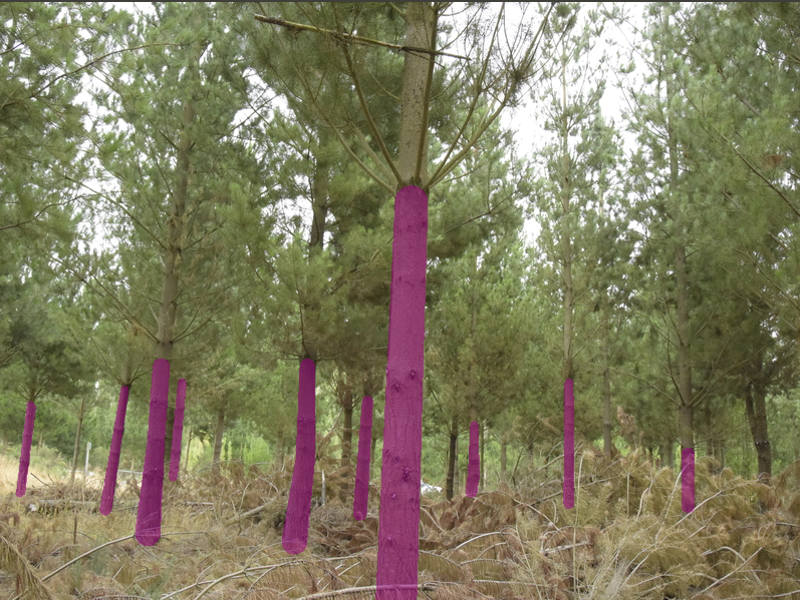
\includegraphics[width=0.9\linewidth]{bootstrap/trees_example.png}

\caption{Example image from the \emph{trees} dataset showing annotated segmentation mask on tree trunks. }
\label{fig:bootstrap_tree}
\end{figure}

\subsection{Related methods}

There are many approximate and interactive machine methods specific to segmentation, in addition to those laid out in Chapter~\ref{chap:introduction}. Each pixel in a mask is highly correlated with its neighbourhood pixels, as such, inputting each pixel is highly redundant; therefore, smart methods can be used to extrapolate segmentation masks from more approximate input. In addition, approximate mask labelling is usually sufficient for most purposes, such as the use of polygons instead of precise boundaries.

An example of active learning specific to segmentation is \cite{Xu2017}, where they focus on finding the nodes (superpixels) which induce the largest change in a \gls{CRF} model.

Semi-supervised machine learning attempts to use existing knowledge or domain properties to infer annotations. For example, using motion cues to give indications of object boundaries \cite{Hong2017}, or using an image classifier to perform object detection by blanking out portions of the image, to determine which parts are important \cite{Bazzani2016}. Semi-supervised methods often substitute for human labour, but in doing so, make sacrifices on the quality and often result in somewhat noisy data. As a result, semi-supervised methods are often used as a means of bootstrapping a model before involving a human annotator, for example as used in \cite{Papadopoulos2016}.


\subsection {Assisted annotation}


\begin{figure}[ht]
\centering
\begin{subfigure}{.5\textwidth}
  \centering
  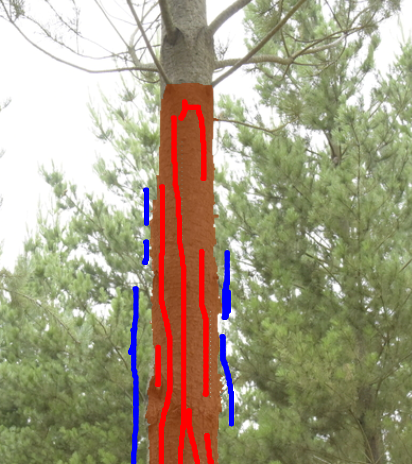
\includegraphics[width=0.9\linewidth]{bootstrap/labelme.png}
  \caption{Labelme mask annotation}  
  \label{fig:bootstrap_labelme}
\end{subfigure}% 
\begin{subfigure}{.5\textwidth}
  \centering
  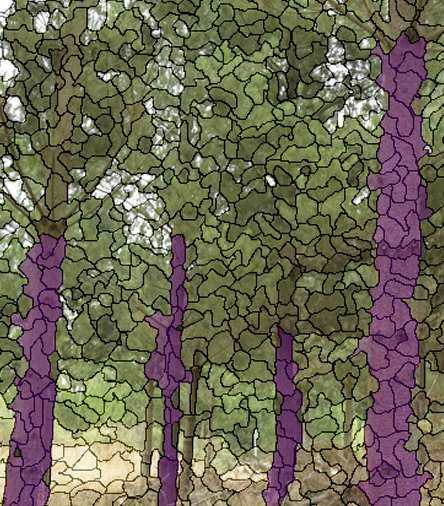
\includegraphics[width=0.9\linewidth]{bootstrap/superpixels.png}
  \caption{Annotation using superpixels}
  \label{fig:bootstrap_superpixels}
\end{subfigure}

\caption{Assisted annotation methods}
\label{fig:bootstrap_annot_method}
\end{figure}


In the initial attempts to annotate a dataset, one of the problems was that using the assisted annotation tools, such as the mask tool in the LabelMe \cite{Russell2007} interface, actually required more work than manually annotating the polygon boundary from scratch. The LabelMe mask tool provides a GrabCut-esque interface where positive and negative stripes can be painted onto an image. Attempts to creating a mask for a tree trunk can be seen in Figure~\ref{fig:bootstrap_labelme}, where annotations are bright red and green. The initially painted stripe provided a rough outline, but many small annotations were needed to make the mask resemble the accurate boundary of the tree trunk.

In \cite{Galloway2017}, the images are segmented using superpixels (clusters of pixels grouped with an unsupervised algorithm), where labelling groups of pixels is substantially less work than labelling individual pixels, and superpixels seem to do well at finding image boundaries where \gls{CNN}s are often imprecise. One difficulty is ambiguity, where multiple classes are covered in one superpixel. In my experience, using superpixels provided imprecise boundaries, and saved little time. An example of the tool with superpixel selection is shown in Figure~\ref{fig:bootstrap_superpixels}.

Deep learning has previously been used to aid in object instance selection. In \cite{Xu2016} a \gls{FCN} is trained to perform semantic segmentation of objects in images as selected by users. Users click on an object (providing positive and negative points), which is provided to the model as distance maps along with the regular colour image data. In \cite{Xu2017} the approach is similar, using a rectangle as an input (also using a distance map), and producing an instance segmentation.


\section{Proposed Method}

The approach is to annotate data and train a model concurrently. First annotate a small number of examples to begin with, to create an initial training set, and use these examples to train an initial model. New examples are then classified by the model, at which point the human annotator fixes any mistakes, and the corrected example is added to the training set. Initially, the annotator will need to fix the majority of the data, and as the model improves such feedback will be required less and less. The idea is that the model will quickly learn the easy cases, which can be quickly ignored to save work, and the annotator will be left to intervene only with the more important challenging cases.

I have used this method to build a small scale tree trunk segmentation dataset, a prototype for use in an automated drone tree pruning project with the aim of pruning lower branches off young \emph{Pinus radiata} tree plantations. This work is intended to allow the drone to see the trees despite the forest. To evaluate methods of dataset construction and evaluate methods of annotation, I wrote an annotation application written with a Qt interface, with tools for drawing on masks and iterating the dataset and refining model proposed annotations.

The work-flow after the first training of some initial  examples was to leave a training process in the background, which would pick up newly created annotations after each training epoch. 

\subsection {Models}

\begin{figure}[h]
  \centering
  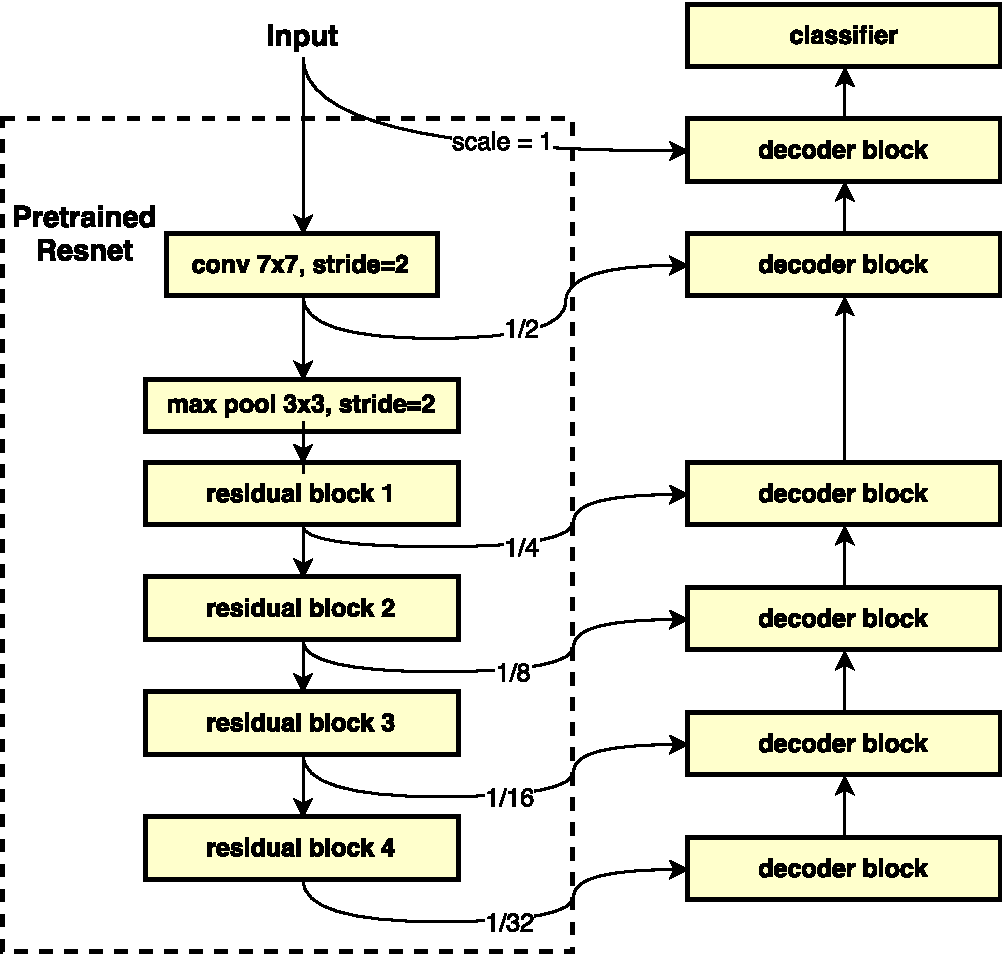
\includegraphics[width=1.0\linewidth]{bootstrap/network.pdf}
  \caption{Encoder--decoder network with pre-trained ResNet as a backbone}  
  \label{fig:bootstrap_network}
\end{figure}
\begin{figure}
  \centering
  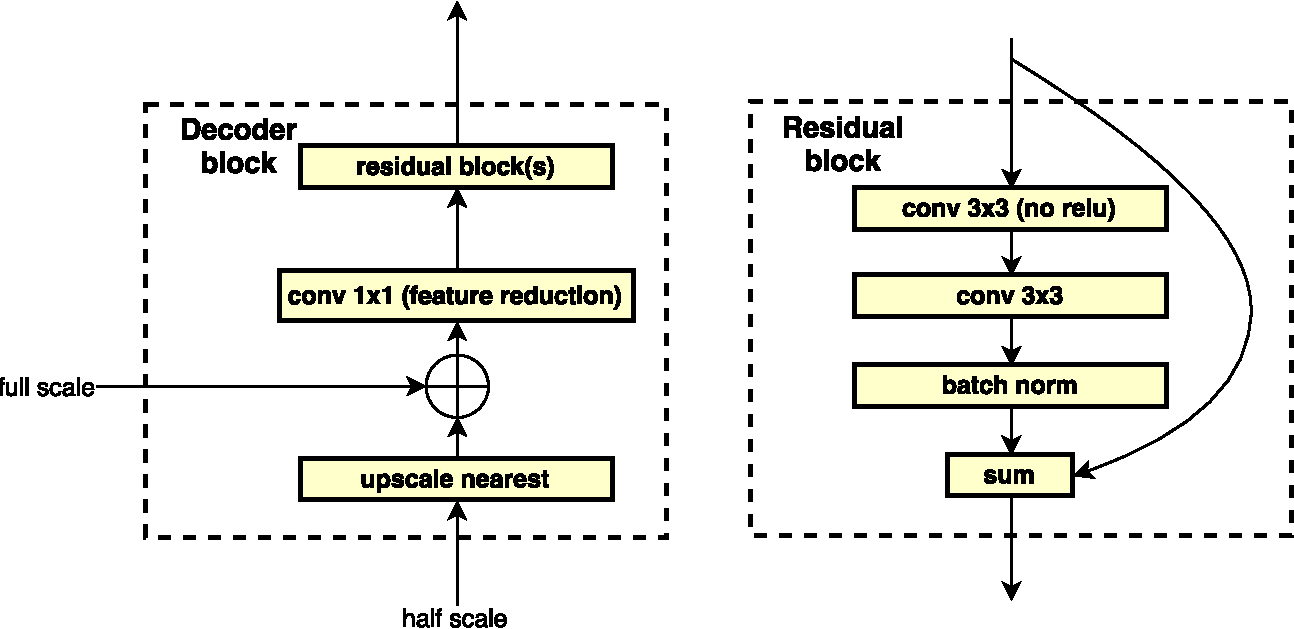
\includegraphics[width=1.0\linewidth]{bootstrap/network_blocks.pdf}
  \caption{Sub-networks. On the left the decoder which combines a low resolution feature map (from a deeper level of the network), with a feature map from the backbone ResNet. On the right the basic residual block with two $3\times3$ convolutions. }  
  \label{fig:bootstrap_decode_block}
\end{figure}

For the image segmentation model, I have used an encoder-decoder with skip connections similar to UNet \cite{Ronneberger2015} (utilising padding and without cropping the skip connections). Each level of the encoder and decoder (at the same resolution) is connected by a skip connection bypassing the lower layers of the network. I focus on two architectures, the first is a pre-trained ResNet model as an encoder with a decoder added, and the second is a symmetrical encoder and decoder. I refer to the first as \emph{pre-trained} and the second as \emph{ladder} in the experiments below.

The architecture based on the pre-trained ResNet \cite{He} is shown in Figure~\ref{fig:bootstrap_network}, with the decoder and residual block used shown in Figure~\ref{fig:bootstrap_decode_block}. The particular ResNet I use is the \emph{ResNet18} from the PyTorch \cite{Paszke2017} model zoo, (the smallest of the various ResNet architectures) with weights trained on the ImageNet dataset. 

The decoder for the pre-trained model uses a single residual block at the point labelled \emph{residual block(s)} in Figure~\ref{fig:bootstrap_decode_block}. The ladder model uses residual blocks of size (1, 2, 3, 3, 3, 3) in both encoder and decoder. The decoder uses $ 1x1 $ convolutions to reduce the feature sizes coming from intermediate layers of the ResNet, the number of features used in the decoder is 16, with 8 additional features at each layer further down. An implicit Batch Normalisation layer and ReLU is present before every convolution.

Of note, the first skip connection is directly the image input, and the second is directly after the $7x7, stride=2$ first convolution used by the ResNet.


\section {Experiments}


\subsection {Loss Function}


I primarily use the \gls{IOU} as a measure of comparison for segmentation. The \gls{IOU} is presented in Equation~\ref{eq:iou} with $ A $ and $ B $ being sets. When training a model, I optimise the Jaccard Distance as a continuous approximation to the \gls{IOU}, this is shown in Equation~\ref{eq:jaccard}.  $ p $ is a binary prediction vector of all output pixels, normalised using the sigmoid function to be between 0 and 1. $ t $ is the binary target vector. Multiplication in these equations is element-wise vector multiplication.


\begin{equation}
IOU = \frac{A \cap B}{A \cup B}
\label{eq:iou}
\end{equation}


\begin{equation}
Jacc = 1 - \frac{p.t}{p.p + t.t - p.t}
\label{eq:jaccard}
\end{equation}



\subsection {Image preparation}

I use images of a fixed size in order to train the network (to process images in batches), however, because the network is a fully convolutional network, inference (and testing) can be performed on images of variable size. I show the effect of this processing later, as compared to training with full-size images with batches of size one.

Data augmentation is used to add variety. I use random scales ($0.8$ to $1.25$), and crops and rotations ($-5$ to $5$ degrees). I adjust colours on a per colour channel basis ($ \gamma = 0.9 $ to $ \gamma=1.1 $ )  $ x_a = x^{\gamma} $.

After scaling and rotation, I then crop an area of the image to $440 \times 440$ pixels (the original image size in the \emph{trees} dataset is $800 \times 600$, down-scaled from the original photos of approximately 25 megapixels).

I employ image whitening as the last step, subtracting an approximate global mean (r, g, b) $ (0.485. 0.456, 0.406) $ and dividing by standard deviation $ (0.229, 0.224, 0.225) $  to ensure consistency with the pre-processing used in ImageNet training with the pre-trained model.



\subsection {Datasets}




I developed a small scale dataset for segmentation of tree trunks in \emph{Pinus radiata} forests (using the approach described). The dataset consisted of 120 images, each containing multiple instances of tree trunks. I labelled the most distinct instances in each image, where some images contained hundreds of background trees. Of the 120 images, I used 30 images for a validation set to use in experimentation in this chapter (which were not used for training).

Along with the \emph{tree} dataset, single classes from the Pascal VOC dataset are used in some experiments. I train with a mix of images from MS COCO \cite{Lin2014} training set along with the Pascal VOC 2012 training set, and use the VOC validation set for validation. The tree images typically contain more instances per image at higher resolution, but significantly fewer images than VOC and COCO images for each category.


\subsection {Minimum viable examples}

\begin{figure}[ht!]

  
\centering
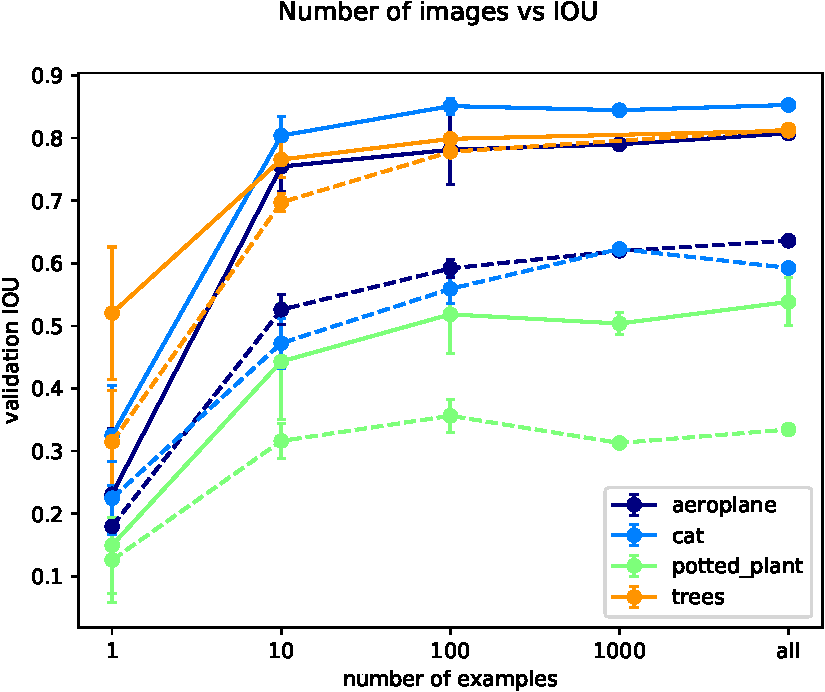
\includegraphics[width=0.9\linewidth]{bootstrap/limit.pdf}
\caption {Validation after training on a limited number of images, solid lines are fine tuned using the pre-trained model, dotted are training from randomly initialisation. }
\label{fig:bootstrap_limited}

\bigskip
\end{figure}

\begin{table}[bht!]
  \centering
 
  \begin{tabular}{ l  l  l}
    examples & training epochs (of 256 images) & repetitions \\
    \toprule
    1       & 8     & 10 \\
    10       & 32     & 4  \\
    100   & 64     & 2 \\
    1000  & 128 & 1 \\
    \bottomrule
  \end{tabular}
  
  \caption{Training parameters for different numbers of examples}
   \label{tab:bootstrap_limit_params}

\end{table}





The effectiveness of involving the model early in the process will be determined by the point where fixing errors in the model's predictions becomes faster than annotating the image from scratch. The effect of the number of examples was studied in \cite{Soekhoe} in the context of transfer learning. One finding was that with smaller numbers of examples, fixing the weights of earlier layers boosted performance when using less training examples.

I performed a simple validation experiment to investigate the effect of using fewer examples. The results can be seen in Figure~\ref{fig:bootstrap_limited}, where in each case the stated IOU is an average over several trials (the number can be seen in Table~\ref{tab:bootstrap_limit_params}), and is additionally averaged over the last three epochs of training. Here I have used classes from the Pascal VOC 2012 for comparison.

It can be seen that even for as few as 10 examples, the validation accuracy is not too different from using a full dataset (1000s of images) in each case, and the difference between using 100 images and the full dataset was minimal in each case. I expected to see the pre-trained model perform much better with a limited number of examples, and this proved to be the case,  it also seems to perform much better in the general case as well. The case matching the initial expectations is the (much more limited) \emph{trees} dataset.



\subsection{Model fine-tuning}

\begin{figure}[!ht]
\centering
  \centering
  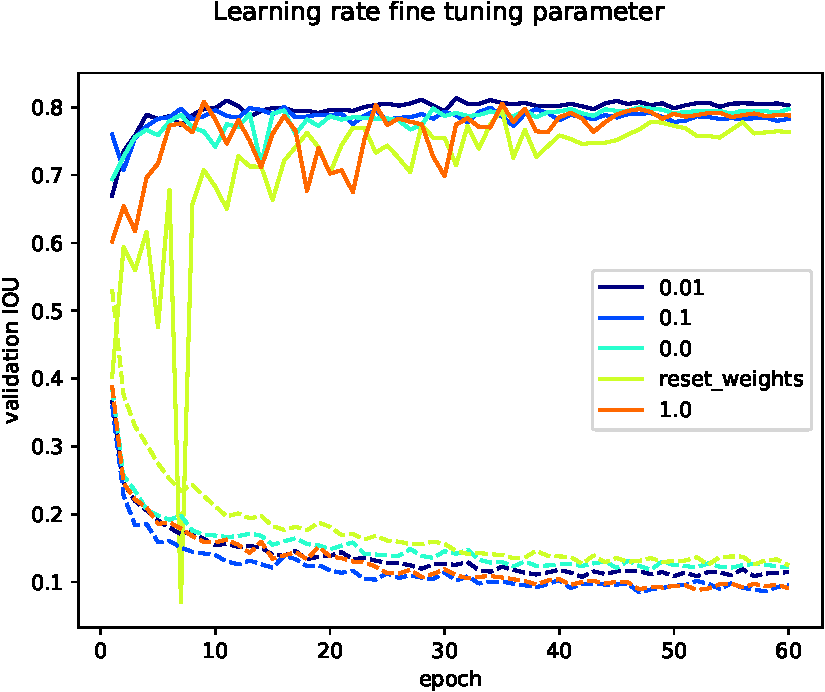
\includegraphics[width=0.9\linewidth]{bootstrap/fine_tuning.pdf}
  \caption{Influence of learning rate modifier for fine-tuning. Solid lines are validation IOU, dotted lines are the mean loss for each training epoch. }  
  \label{fig:bootstrap_fine}
\end{figure}


\begin{figure}[!ht]
  \centering
  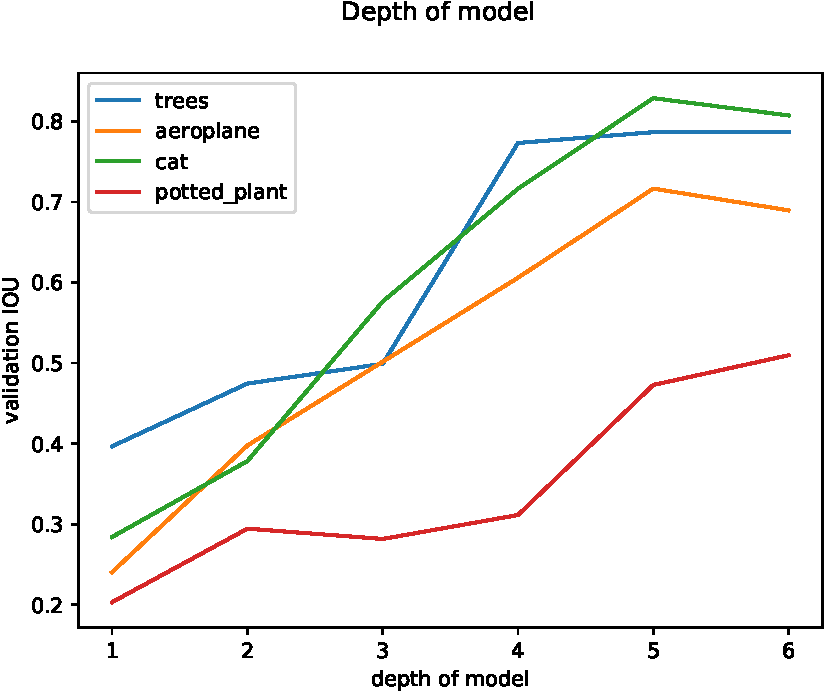
\includegraphics[width=0.9\linewidth]{bootstrap/depth.pdf}
  \caption{Depth of pre-trained model}  
  \label{fig:bootstrap_depth}
\end{figure}


I examined the best parameters for fine-tuning, finding that allowing a small learning rate on the pre-trained model was advantageous. The effects can be seen in Figure~\ref{fig:bootstrap_fine}, where $0.01$ (fraction of the learning rate used for other parts of the model) was advantageous. I used $ 0.1 $ for all other experimentation in this chapter. It can be seen that without the lower learning rate, the pre-trained parameters are disturbed, leading to lower validation accuracy, and without any fine-tuning, the pre-trained parameters are not able to adapt.

Depth of the model is examined, and I experiment with truncating the pre-trained model. Results can be seen in Figure~\ref{fig:bootstrap_depth}, where the depth of the model had a strong positive effect on the output of the model. Given these results, I might consider using a model with even more depth scales. Given the number of convolutions (especially at the lower scales), the ResNet--18 model I have been using has quite a large receptive field, and with more depth scales the receptive field would be larger. In \cite{Peng2017} benefit was found in using very large kernels at the lower levels of the model specifically to enlarge the receptive field.






\subsection {Partial Annotation}


\begin{figure}[!ht]
\centering
\begin{subfigure}[t]{.33\textwidth}
  \centering
  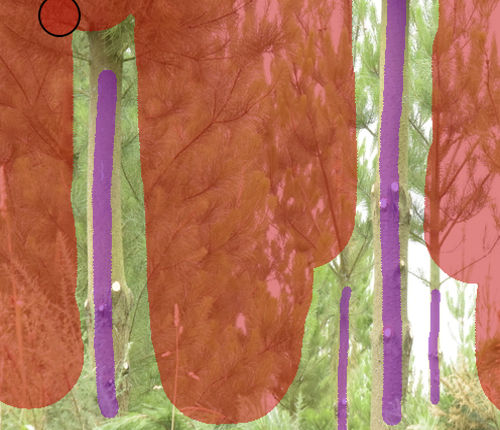
\includegraphics[width=0.9\linewidth]{bootstrap/loose.png}
  \caption{Partial annotation}
  \label{fig:bootstrap_loose_annot}
\end{subfigure}%
\begin{subfigure}[t]{.33\textwidth}
  \centering
  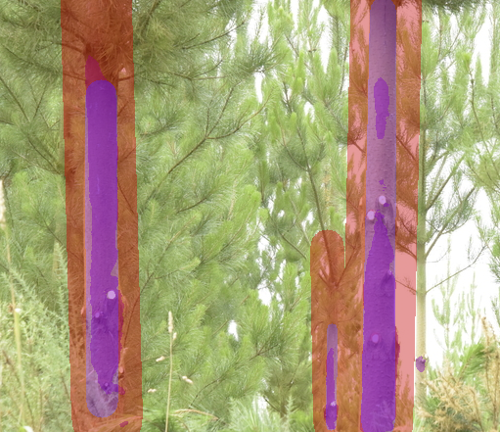
\includegraphics[width=0.9\linewidth]{bootstrap/loose_directed.png}
  \caption{Directed annotation}
  \label{fig:bootstrap_loose_dir}

\end{subfigure}%
\begin{subfigure}[t]{.33\textwidth}
  \centering
  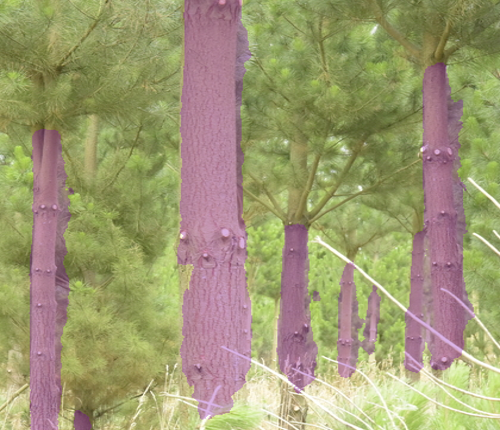
\includegraphics[width=0.9\linewidth]{bootstrap/loose_predictions.png}
  \caption{Partial inference}
  \label{fig:bootstrap_loose_pred}
\end{subfigure}
  \caption{Loose annotation methods in (a) and (b), the red overlay is pixels labelled as background where transparent pixels are unlabelled, (c) shows the  noisy outline produced from partial annotation }


\end{figure}

\begin{figure}
\centering
\begin{subfigure}[t]{.33\textwidth}
  \centering
  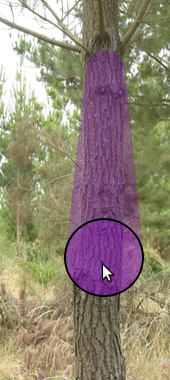
\includegraphics[width=0.6\linewidth]{bootstrap/line_tool.png}
  \caption{Line tool}
\end{subfigure}%
\begin{subfigure}[t]{.33\textwidth}
  \centering
  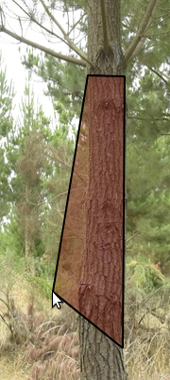
\includegraphics[width=0.6\linewidth]{bootstrap/polygon_tool.png}
  \caption{Polygon tool}
\end{subfigure}%
\begin{subfigure}[t]{.33\textwidth}
  \centering
  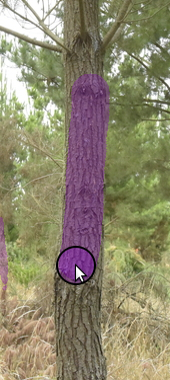
\includegraphics[width=0.6\linewidth]{bootstrap/paint_tool.png}
  \caption{Paint tool}
\end{subfigure}%

  \caption{Label paint tools used in annotation}
  \label{fig:bootstrap_tools}

\end{figure}



An alternative to densely annotating every pixel in an image is to selectively label some pixels while leaving many unlabelled - in the vein of the GrabCut algorithm. I examine this idea for two reasons, firstly annotation of all pixels is finicky or ambiguous (such as the small trees in the background), and secondly to optimise time spent on the annotation of only the most informative pixels (in the vein of active learning).

I firstly looked at partial annotation using paintbrush scribbles on the centre of trees and around the edges of the background. It can be seen that the model trained with partial annotation does not accurately find tree boundaries and has reduced precision as a result, as can be seen in Figure~\ref{fig:bootstrap_loose_pred}. After identifying flaws in that process I compared directed annotation, where I trained a model as I went, in order to guide the annotation process.

For directed annotation, I aimed to densely label the tree instances only where there were mistakes, otherwise leaving the rest of the image not annotated. At the points where mistakes occurred, I made sure to capture the boundaries more accurately. I was again annotating only a small number of easier instances where annotation was clear, unlike in the dense annotation case where many small and ambiguous instances are labelled.

Some statistics can be seen in Table~\ref{tab:loose_exp}, where I can see that both methods of partial annotation are less effective than dense annotation. The second method of directed annotation improves on the precision but reduces recall. It can be seen that the extra supervision of background pixels is indeed useful, and useful supervision is lost by not including it.


\begin{table}[!ht]
  \centering
    \caption{Statistics from re-annotation test set with different levels of approximated annotation, where some pixels are ignored to save annotation time. }
    
  \begin{tabular}{ l  l  l l l l l }
    method & \shortstack{positive \\ pixels}  & \shortstack{background \\ pixels} & \shortstack{ignored \\ pixels} & precision & recall & IoU  \\
    \toprule
    dense annotation    & 10.4\% & 89.6\% & 0\% & 87.8 & 87.3 & 77.8 \\
    loose annotation    & 5.2\% & 67.4\% & 27.4\% & 82.3 & 83.3 & 70.7 \\
    directed annotation & 7.2\% & 54.9\% & 38.0\% & 87.7 & 80.7 & 72.5 \\    
    \bottomrule
  \end{tabular}

\label{tab:loose_exp}
\end{table}

\subsection {Annotation interface experiment}

I performed an exercise in re-annotating the validation set using different tools. The results can be seen in Table~\ref{tab:annotation_exp}, where I used three approaches. The different tools used can be seen above in Figure~\ref{fig:bootstrap_tools}.  The first being a duplication of the initial annotation using the line tool (the tool I initially used to label the dataset), the second being a polygon tool (more commonly used and general purpose than the line tool), and lastly I refined images produced by a trained model, fixing mistakes using the paint tool.

The model I used was a model trained on 30 images (densely labelled) from the loose annotation experiment above. I can see the method of refining model predictions is somewhat faster than the other two input methods, but due to the exercise being undertaken by a single user it is not significantly different ($ p > 0.01 $).

During the annotation, I showed an image of the existing validation image and its annotations side by side to the annotation software, which was necessary to ensure the same task was being performed. The smaller instances in each image were subject to the judgement of the annotator, and other images were extremely crowded or blurry, leading to ambiguity in the annotation process. 

I consider human variability, using a reference annotation created with the same tool operated by the same user. The annotation compared to the reference, only manages a precision and recall of approximately $90\%$. All three input methods were similar in this regard, but display different bias. The polygon tool, for example, was more precise but less complete (lower recall), indicating that the user tended to cut within boundaries defined by the original labelling. 
 
\begin{table*}[!ht]
  \centering
    \caption{Statistics from annotating the set with polygons, lines and then by refining model predictions. Precision, recall and IOU are a comparison with the original validation set. Note figures in brackets are the original statistics of the unmodified predictions from the model}

\noindent\resizebox{\textwidth}{!}{%    
  \begin{tabular}{ l  l  l  l  l  l  l  l }
    method & \shortstack{time \\ per image (s)} & \shortstack{edits \\ per image (s)} & \shortstack{pixels \\ per image} & \shortstack{time \\ per edit (s)} & precision & recall & IoU \\
    \toprule
    polygon    & $79.3 \pm 35.0$  & $12.1 \pm 5.6$ & $52438 \pm 31900$   & $3.9 \pm 1.8$  & $0.94$ & $0.88$   & $0.84$ \\
    line         & $71  \pm 33.4$   & $12.2 \pm 5.6$ & $54781 \pm 33336$   & $2.1 \pm 1.4$ & $0.92$  & $0.90$  & $0.84$ \\
    refine     & $57.3 \pm 40.3$  & $10.8 \pm 6.1$ & $6561 \pm 7102$       & $1.7 \pm 1.4$ & $0.92 (0.89)$   & $0.92 (0.85)$ & $0.85 (0.77)$ \\    
    \bottomrule
  \end{tabular}
}

\label{tab:annotation_exp}
\end{table*}


The confounding feature in the annotation experiment was the need to look backwards and forwards between the two images in order to ensure the correct areas were annotated. In images with many instances, this became a difficult task and identifying small differences between the two became much more difficult. In future, I may perform a more comprehensive user study, by providing an outline of the desired mask for the user to copy directly. This way, the user does not spend any time comparing images and can focus only on the interaction (as a regular user of the annotation tool would).


\subsection{Practical considerations}

Hyperparameters, for example, training rate and model architecture, still need to be determined by validation as soon as enough examples have been obtained to be feasible. I performed some tuning of the hyperparameters (for example the crop size, data augmentation parameters, learning rate) for the purposes of the experiments in this chapter, using the person category of the Pascal \gls{VOC} 2012 dataset; despite the fact that the \emph{tree} dataset is significantly faster to train a similar set of hyperparameters seems to have been suitable.


Practical considerations of having a training process for a \gls{CNN} in the background is that it uses a lot of both \gls{CPU} and \gls{GPU} resources. Running the trainer and the annotation tool together caused significant lag in the annotation tool, which was not otherwise present. It was especially noticeable with a large batch size when the tool would lag in sync with each batch processed. The effect was that annotation became more time-consuming. A simple solution to this would be, for example, to run processes on different machines with a web interface.


\section{Future work}

The interest in tree segmentation was initially for robotic pruning applications and navigation. For this purpose, the segmentation requires further interpretation and fitting. For example, in order to identify tree instances, groups of pixels can be identified then fitted to oriented boxes. This approach does not work for overlapping trees; however, object detection methods also typically struggle with highly overlapping objects.

For these reasons the direction I pursued was to take some of the ideas and lessons learned and apply them to object detection, as can be seen in chapters~\ref {chap:object_detection} and~\ref {chap:annotation}.

For purposes such as identifying foliage of the trees or looking at obstacles in the forest, segmentation does seem like the most natural fit; where one object cannot be easily separated from another. For example, the \emph{Pinus radiata} needles are not distinguishable in the canopy as to which tree they are attached.

\subsection{Segmentation specific}

There is considerable scope for assisted annotation of segmentation datasets, specifically, because the annotation of each pixel is especially laborious. Here are some potential future directions: 

\begin{itemize}
    
\item  {\bf Interactive segmentation} \par
Segmentation often has a class-agnostic element, where the boundary of an object is clear regardless of the object type. User hints can often resolve any ambiguity. An example is interactive object selection \cite{Xu2016, Xu2017}, where user input is combined with image data to segment an object. Large segmentation datasets combined with simulation are used for training, however, an iterative refinement on the specific dataset during annotation may bring further benefit.

\item  {\bf Object selection} \par
Object selection algorithms that can work on the features or outputs from \gls{DNN}s is another idea, such as higher dimensional GrabCut \cite{Xu2016a}, or SuperPixels. Performing Features learned from pre-training on large image datasets is also possible.

\item  {\bf Polygons or shapes} \par
Pixel masks are rarely fully accurate, and drawing tools provide approximate methods for inputting masks in the first place. Directly predicting the kinds of shapes used to input annotations might be a better alternative such as polygons, for example, used in PolygonRNN \cite{Castrejon2017}. Like pixel masks, polygons can be produced by a \gls{NN} and refined by a human annotator. Polygons can be manipulated more easily and better represent the fact that the boundary is an approximation.
\end{itemize}

\section {Summary}

I proposed a bootstrapping method for rapid segmentation dataset creation, involving a feedback loop between human and model. The model trained on partial data was used to assist a human annotator, who then verified the model's predictions and fixed any mistakes. I used this method to create a \emph{tree} dataset for segmentation of \emph{Pinus radiata} trunks (to find trees requiring pruning). I then performed several experiments on this dataset, as well as the Pascal VOC in order to see how I might improve on this bootstrapping method. 

Through several experiments, I determined that fine-tuning a pre-trained model was an effective way to obtain a workable model with very few input images, at least on the \emph{tree} dataset. Partial annotation was explored and found to be less effective than a dense annotation. For this reason, I think that it is more useful to create tools to assist the user to create a dense annotation, rather than making do with more approximate labelling. 

% \setcounter{chapter}{4}
% \chapter{Design-Implementation}
\label{chap:design} 

\section{Introduction}

This chapter describes the design and implementation of a human-in-the-loop verification based annotation system. The interface is similar to a diagram editor, however, at each step the machine model is integrated as seamlessly as possible to evaluate the easy cases and leave the annotator to verify and correct only the harder cases. 

I discuss some novel methods such as using the machine model to assist in reviewing annotations for quality assurance and also discuss a novel method for utilising weakly detected objects.

I later describe the implementation, which is written as a web application for ease of distribution and usability. The implementation is split into three parts, firstly, a web based client, secondly, training processes running on machines with powerful \gls{GPU}s and thirdly, a server acting as an intermediary that is storing image data, user actions and parameters of trained object detection models.

\section {Goals}

The goal of any annotation system is to efficiently and accurately allow a user to annotate a set of images. The main consideration was to be of practical use for real problems. From experience gained during work on chapter~\ref{chap:bootstrap} I set out to achieve some specific goals (some developed more than others in this work):

\begin{itemize}

\item {\bf Object detection} \par
While segmentation is appropriate for some specific tasks, notably where elements of interest are described by irregular shapes, object detection and variations are more generally useful. The goal is not just bounding box object detection but other annotation types such as polygons, for instance, segmentation, oriented boxes, lines and custom types of pose/keypoint estimation.

\item {\bf Verification based annotation} \par
Of methods explored in chapter~\ref{chap:bootstrap}, using human verification and correction of machine predictions seemed the most promising. Therefore the goal is to integrate this idea as seamlessly and unobtrusively as possible, 

\item {\bf Flexible use} \par
To be generally useful, a tool needs to work well in a variety of situations without needing a lot of special tweaking. Some of the focuses in this work have been to adapt to different image resolutions, very small objects, and objects which are abundant or sparse. 

\item {\bf Easy deployment} \par
In chapter~\ref{chap:bootstrap} a C++ application was used for annotation. Two issues can be identified, firstly hardware and complex dependencies, and secondly the interactivity impairment of running GPU processes on a local machine. Along with all the dependencies required to train the model (PyTorch \cite{Paszke2017} and all its dependencies) and the \gls{GPU} requirement; it is clear that for people to use such a system a simple method for deployment is preferable. For these reasons I focused on a web application which can run on a server with a GPU, then be accessible by anyone from anywhere.

\item {\bf Support experimentation} \par
While one goal is to reduce the amount of manual tuning necessary for most use cases, the goal is to be able to empower an annotator to get the best results from the data. This comprises  several parts: (a) the ability to get feedback, both automated in terms of testing and visual feedback on new data; (b) the ability to modify parameters, and see the results, for example, parameters change the training image size, or adding another class category; (c) to be able to organise data in useful ways, for example, to be able to filter and search, based on automated detections on new data.

\end{itemize}


Other ideas have since become more of a focus after using the system in practice, two of the most important ones being:

\begin{itemize}

\item {\bf Active learning and image selection} \par

It became apparent through experimentation (see chapter~\ref{chap:annotation} that in some dataset types, such as those where object instances are less uniform, selecting the right parts of the dataset to annotate first becomes important. Active learning also presents an opportunity to synergise with \gls{VBA}, as many images containing uncertain detections may also contain many easy to detect objects.

\item {\bf Reviewing and cross verification} \par

Given the importance of ensuring correctness in annotations, and the risk of algorithmic bias using a \gls{VBA} system (where a user may fail to correct a mistake in the machine annotated image), finding methods of validating annotations becomes important. 

\end{itemize}


\section {Verification based annotation}

At the core of the user interface is the use of an object detector seamlessly providing immediate feedback on images viewed by the user. When a previously unedited image is opened, the model simply provides the set of predicted detections which are presented to the user for verification. 

In the first implementation, this was a manual operation where a user viewing an image could click a button to retrieve model predictions. This adds an unnecessary action, although it does make it apparent to the user where the annotations came from. One downside to the seamless auto detection and review interface, is that it is not necessarily obvious if the annotations being viewed are the result of model predictions or user inputs.

\subsection{Basic operation}


\section {User interface}
\label{sec:user_interface}
 
The user interface of the system resembles a diagram editor, where annotation shapes (boxes, circles or polygons) can be drawn over an image and manipulated in the usual ways. Shapes can be moved by selecting and dragging, re-sized by scrolling the mouse wheel or by dragging control points. 

\begin{figure}[h!]
  \centering
  \includegraphics[width=1.0\linewidth]{figures/annotation/penguin_refine.pdf}
  \caption{Illustration of a human annotator refining a set of bounding box predictions. The boxes modified at each step are highlighted (corner markers shown and shaded). The image used is from the \emph{penguin dataset} \cite{PenguinData} }   
  \label{fig:penguin_refinement}
\end{figure}

An illustration of the annotation process is shown in figure~\ref{fig:penguin_refinement}, showing the user refining a set of bounding box annotations. The diagram illustrates the main operations available to the annotator, which are:

\begin{itemize}
    \item {\bf Transform bounding box}\par
An inaccurate bounding box can be corrected by clicking and dragging a corner or moving its centre by clicking on the box as a whole and dragging it. The scale may also be adjusted at the same time by scrolling the mouse wheel.
    \item {\bf Confirm weak detection}\par
If the \emph{review} mode is activated, detections of weak confidence will show with dotted lines. I use a two confidence level threshold system (see section~\ref{sec:thresholding}). A user may then click on the box to confirm it as an annotation.
    \item {\bf Delete box}\par
Any false-positive predictions from the object detector, which meets the threshold as a high confidence detection, can be deleted by selecting the box (by clicking on it) and pressing a key. 
    \item {\bf Draw box}\par
For objects in the image completely missed by the object detector, the user may draw a box by holding a key then clicking once on one corner, and again on the other corner.
    \item {\bf Change class}\par
The class of a box annotation may be changed by selecting the object and then selecting the active class. The best method for this is to setup hot-keys for some of the more commonly used classes.
    \item {\bf Submit image}\par
Once the image has been corrected to the required standard, the user may then submit the annotated image where the annotations are saved and immediately used for training.
\end{itemize}

Some of the operations above may be conflated, for example, low confidence predictions are sometimes not localised well - so the user may transform the bounding box at the same time as confirming the weak detection.


Multiple annotations can be selected together using a rectangle select, and moved or deleted in one action.  This saves a lot of time when the model creates excessive extraneous detections which occur frequently when an image contains objects of a scale previously unseen, or is containing content from a distribution previously unseen by the model. \gls{CNN} models are known to produce false positives on out of distribution images \cite{Hendrycks2016,Lee2018}. This property also enables adversarial attacks on \gls{CNN} classifiers. An example in the \emph{Scallop} imagery was when querying predictions on an image containing a (previously unseen) diver.



\subsection {Navigation}

Navigation is crucial to being able to effectively examine an image (and thus annotate it well). The ability to zoom into a portion of an image to view it more closely and see details is important,  particularly  for parts of an image with higher uncertainty. Equally important, is the ability to zoom out to view the whole image in order to check for missed details. 

A zooming/panning interface similar to Google Maps is provided where panning is achieved by clicking and dragging, with zooming achieved by use of the mouse wheel. The zoom centres around the mouse cursor so that the image at the mouse cursor is fixed.

Fitts's law is the generally accepted model to guide pointing performance where pointing time is determined by an \gls{ID} $ ID = log_2 \frac{2D}{W} $ where D is the distance to travel and W the width of the target. This has direct consequences for annotation where the edge of a box is a narrow target for selection. 

The zooming and panning interface facilitates faster target acquisition (by reducing D and increasing W), however, in order to verify the correctness of the entire image annotation, a user must also consider the image as a whole when deciding when to submit the image. If the image has too many instances or potential instances of the target object, the risk is that the user misses some or does not remember accurately where they have checked. 


\subsection {Video Annotation}

Many image datasets are either time series (for example images taken minutes apart), or are derived from video.  Approximately half the annotated datasets described in this work (see chapter \ref{chap:annotation})  are derived from video, and of those remaining, two are time series. Functionality for the annotation of video sequences is limited in this work, however, organisation of images in order of time (and frame sequence) is provided, and the ability to view a small amount of context in time around a current frame is supported (by use of shortcut keys).

Viewing context helps avoid ambiguity from an annotation perspective, as often in a video sequence, if something is unclear from a single frame it is possible to resolve that ambiguity by viewing back or forward in time. An example of this is in the \emph{seals} dataset (described in chapter~\ref{chap:datasets}) where identifying a pup next to a mother is often somewhat ambiguous, but viewing the movement over time usually resolves the ambiguity.

Although many promising directions exist to utilise temporal and spatial consistency, for example, using tracking or interpolation between annotations, this work treats every image independently. 


\section {Which detections to show?}
\label{sec:thresholding}

Showing the right number of detections is an important factor. The consequence of showing too many or too few detections causes extra work for the annotator, either by needing to delete too many false positives or having too many boxes to draw. Object detection typically uses a threshold on confidence. If the confidence is set too high there are too many true positive detections hidden, and if set too low the interface becomes cluttered with many false positives.

In \cite{Fitchett2013} a method of predictive highlighting items in a file browser was shown to improve access times. When annotating an image the missing annotations are not always obvious. A weak object detector often shows many spurious detections and it often highlights image areas hiding more uncertain examples, acting like the predictive file highlighting effect. For this reason I seek to make use of all the detections, even for just highlighting areas of interest to a user. 

\subsection{Making use of weak detections, dual threshold method}

 Many times, especially with difficult image detection problems, a weak detector will still produce many detections (some true positives, some false positives). The weak detector will not be able to separate these detections by confidence value. By using human verification there are some obvious strategies to separate the true positives from the false positives, while still not missing too many objects altogether. 

\begin{itemize}
    \item Set a low detection threshold and have the user delete false positives
    \item Set a low detection threshold and have the user select true positives
    \item Set a high detection threshold and have the user draw boxes around missed detections
\end{itemize}

Each of these strategies has a valid place. If detections are so noisy and if the location predictions are also very noisy (for example, when the detector is very weak, such as near the start of the process) - having the user draw boxes is often the only option. Some of these strategies are among those used by \cite{Konyushkova2017} where attempts are made to solve this problem differently, by automatically determining the best interface for a given image.

Deleting false positives is often the best option if true positives outnumber the false positives, or if the false positives are easy to select (if they're grouped together, for example). Selecting true positives is often the best option if the false positives outnumber the true positives. 

Another strategy exists, which has the best of both worlds. Two thresholds can be used, a high confidence threshold for eliminating false positives (so that when using this threshold the number of false positives is low), as well as a low threshold. Detections between the high and low confidence thresholds can be considered for selection as true positives (so that the number of true positives requiring selection is low).


\begin{figure*}[h]
\centering
\begin{subfigure}[t]{0.5\linewidth}
  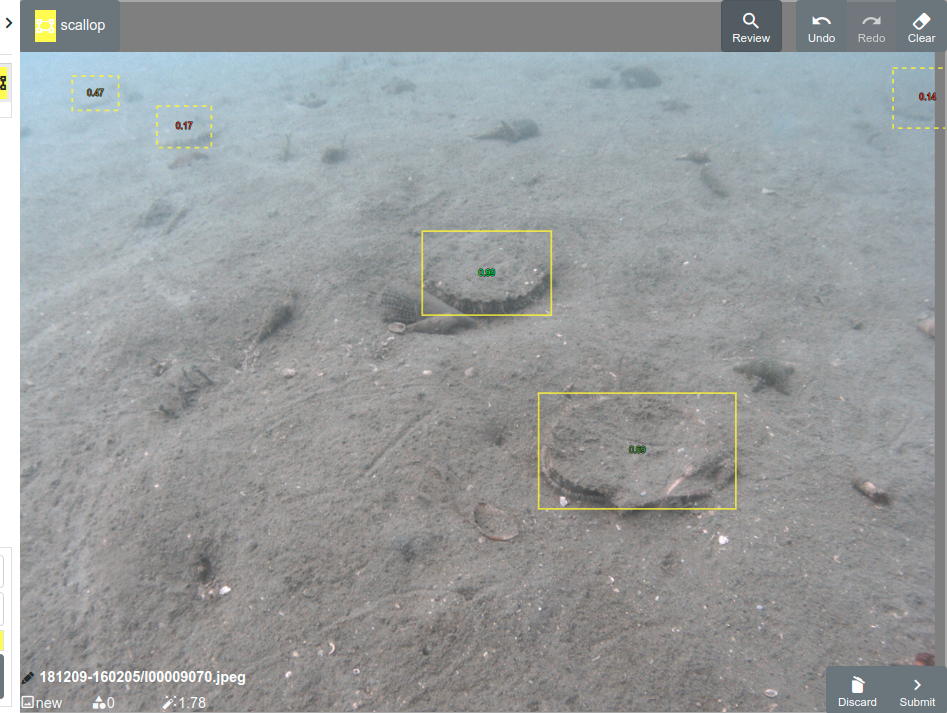
\includegraphics[width=1.0\linewidth]{figures/annotation/scallop/review_mode.png}
  \caption{}
\end{subfigure}%
\begin{subfigure}[t]{0.5\linewidth}
  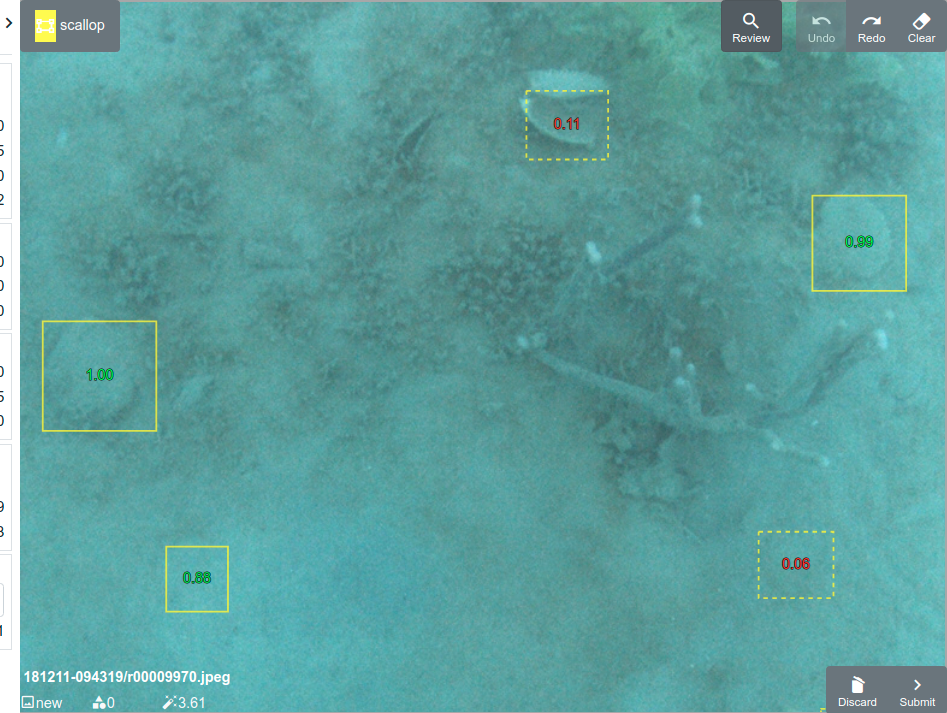
\includegraphics[width=1.0\linewidth]{figures/annotation/scallop/false_positive.png}
  \caption{}
\end{subfigure}%
\caption{Review mode used on two fresh images from the \emph{scallop} dataset, (a) showing an ideal case (b) showing an image with a high confidence false positive among low confidence detections}
\label {fig:scallop_review}
\end{figure*}


I provide a key which toggles \emph{review mode} on which shows weakly confident detections which lie above a minimum threshold but below the threshold for a confident detection. When the key is held, a click is used to confirm a detection as a true positive. I term this toggle \emph{review mode}.  An example showing the use of this can be seen in figure~\ref{fig:scallop_review}. In one image the ideal situation is shown where three scallops are detected in the background (with low confidence), where otherwise they might have been ignored. In the other, a less useful case, where the low confidence detections are false positives, and one of the high confidence detections is also a false positive, but despite this the user saves time by ignoring the other low confidence detections.

The other advantage of this strategy is that it can bring the annotator's attention to areas of the image which may have gone unnoticed. I have noticed in particular with the underwater scallop images, that the detector usually did a good job at bringing attention to the more uncertain scallop instances. It also provides useful feedback to the annotator of the progress of the current object detector. 

During training it can be seen that the confidence levels provided by the object detector vary with regard to training time. This is a known property of neural network classifiers \cite{Guo2017}.

In future, I would like to investigate calibration of thresholds using validation so that the user doesn't have to do this. One method is to adjust thresholds to match a certain ratio of false positives to false negatives (the desired ratio to be set by the user), alternatively, prediction confidence itself can be calibrated to attempt to provide more consistent values. Confidence scores can be calibrated by scaling outputs prior to applying softmax normalisation \cite{Guo2017}. For the purpose of object counting I use the former method to select thresholds. In order to provide the most unbiased estimate of counts, the confidence is selected to give an equal ratio of false positives to negatives.
 
\section{Image/example selection}
\label{sec:example_selection}

While not the core focus of this work, active learning and example selection is complimentary to verification based annotation. Both attempt to remove the burden of labelling all the easy cases in a dataset. Active learning seeks to have the annotator label the most informative images by example selection, and verification based annotation attempts to achieve the same thing by automatically labelling the easy cases so the human annotator does not have to. 

In object detection datasets, many images contain a mixture of easy and difficult examples, so it makes sense to use both active learning and a verification based annotation.  Firstly, active learning example selection picks images containing uncertain object detections, then secondly, a verification based annotation approach is taken to annotate the uncertain image, where the user needs only annotate or correct the hard cases where the model performs badly.

I have implemented a number of simple metrics for selecting images based on heuristics which I have found useful in different kinds of workflows. For example in sparsely populated images, such as in the scallop imagery, to best utilise annotator time, it seems prudent to present images containing (or believed to 
contain) scallops first. Another example is annotating a single class (or few classes) from a much larger image set, where only a subset of the images contains the object in question.

Very recently, published measures of uncertainty for object detection (for example using Bayesian \gls{NMS} \cite{Harakeh}), ensembles \cite{Le2018}, or test time augmentation \cite{Wei2018}) give a future direction to integrate uncertainty approaches. Using cross-validation with an ensemble of models seems promising, although it will increase the training time.

\subsection {Image Implementation}
\label{sec:example_implementation}

Three main image selection policies exist: (a) select images in sequence, either by time, video frame or file-name; (b) select images at random; (c) select image by heuristic. When an image is submitted, the next image is chosen according to the policy enabled, from the set of unlabelled images not being annotated by any other user.

When example selection by heuristic is enabled, the trainer will evaluate a random sample of unseen images (images not yet annotated or discarded) for object detection at each training iteration. Object detections are then evaluated according to the heuristic and ranked  for annotation ordering. 

In general, evaluating the entire image set of unlabelled images for each training iteration is usually far too slow, so using random sampling often ensures a more balanced set of training examples. Too much reliance  on a heuristic may result in many similar images being selected, causing an imbalance in the training set.

For certain kinds of heuristic, such as frame variation (discussed below), it is necessary to evaluate many frames in sequence. For this there currently exists a manual operation where a user can schedule a full evaluation of the set of images. This evaluation can take a long time for a large image set, and occurs much less frequently during the annotation process.


\subsection {Image selection heuristics}
\begin{itemize}
\item {\bf Detection score. }

For this I use the sum of squares of the confidence scores, $ \sum_(p \in detections){ p^2 } $ where $p$ is the confidence for a given detection. 

    \item {\bf Count variation. } \par
Used with object counting datasets, where the sensitivity of the count in each image is used. Images with the widest difference in count at two thresholds are selected first, the two thresholds determined on the validation set to give $ \pm 10\% $ counts.
    \item {\bf Frame variation. }  \par
In time sequence and video datasets, the variation in count between nearby frames can be used to estimate uncertainty. For this I use the difference between a frame and a running average for a window centred around that frame. For this, the metric is determined after predictions for all frames are computed, and counts estimated.
    \item {\bf Training error. }  \par
Making use of the loss from training was proposed for the purpose of finding training images with error. Initial experiments with this indicate the object detection models manage to fit images, even with the most obvious mistakes, with low loss, making this form of example selection less useful. In future using a k-fold cross-validation training ensemble is proposed such that each image is left out of training for at least one model, allowing an unbiased comparison with at least that model.
\end{itemize}


\section{Browsing, sorting and reviewing images}
\label{sec:browising}


\subsection{Reviewing images}
\label{sec:reviewing}

In crowd sourcing image annotation software, quality assurance is usually performed using cross verification, where  either multiple users annotate the same images, or each image passes a set of checks performed by other users before the quality is deemed acceptable. Verification prevents malicious or incompetent users from spoiling the data and provides some assurance that the end result is of high quality. In this work I prototyped the idea of using the trained model to assist with quality assurance by (a) finding images to review (see section~\ref{sec:example_selection}), and (b) illustrating inconsistencies with the trained model.

When a previously annotated image is opened, the existing annotations are matched with model predictions, and interface functions similarly to a difference viewer (version control) for image annotations. Matches are determined by a greedy matching process as used for evaluating object detection, described in section~\ref{sec:evaluation_metrics}. The user can view these changes by toggling the \emph{review} mode on and off. This functions in a similar way to the initial refinement process where the \emph{review} mode is used to show detections of weak confidence. 

Where model predictions differ from the provided annotations, a dotted outline is shown. This highlights annotations where the localisation differs from model predictions, as well as potentially missed annotations. A confidence score is also shown on existing annotations, highlighting annotations for attention which are either missed by the model, or are potentially errors in annotation.

The difficulty faced with using the trained model to determine annotation inconsistency, is that the model tends to overfit the training data. In order to adequately use a trained model for this purpose, the image must not be one used directly in the training process. With the current design, this restricts the use to images in the validation set. In future the plan is to use k-fold cross validation, so that each image is left out of training with at least one model. 

It is anticipated this form of quality assurance will prove more useful with a larger number of training examples and thus more accurate object detection models. It may be useful as just one part of a quality assurance system, allowing a user to quickly identify parts of an image which require attention. Further work is required before these ideas can be evaluated properly (and in this thesis I make no attempt), and this will likely occur be more important for larger scale annotation efforts.

\subsection {Sorting}

\begin{figure}[!h]
  \centering
  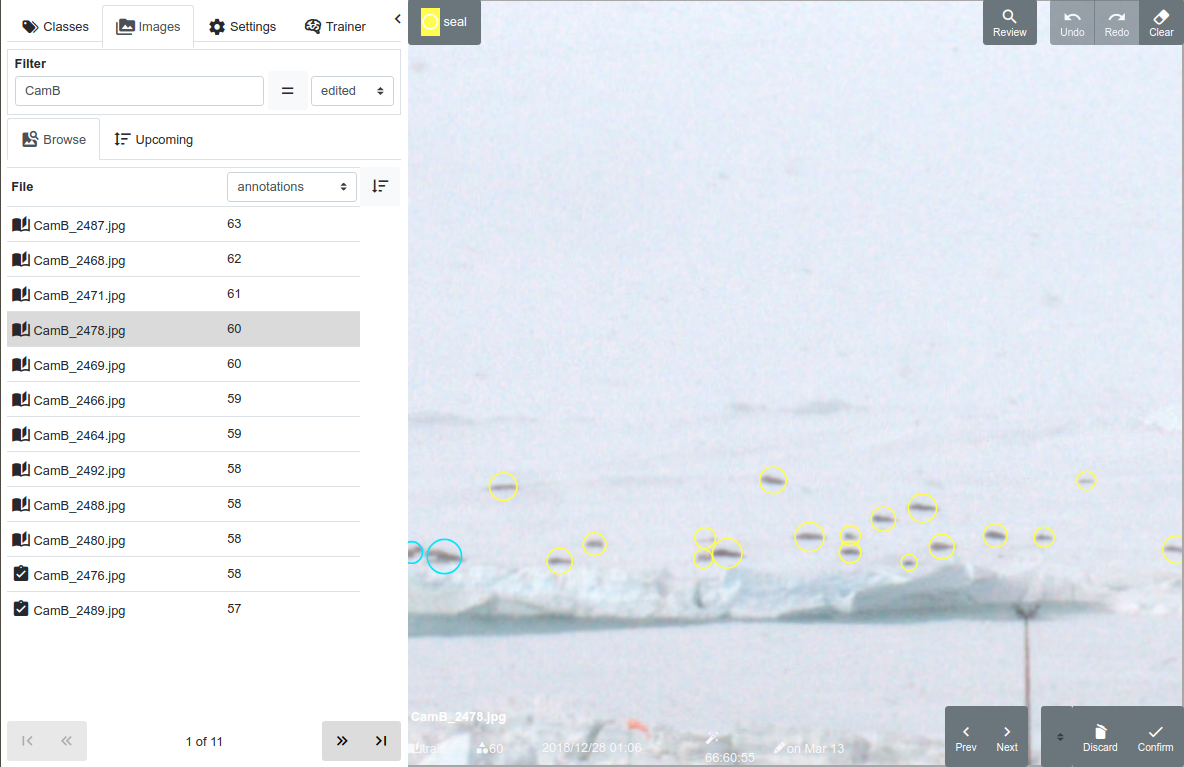
\includegraphics[width=1.0\linewidth]{figures/annotation/screenshots/sort_filter.png}
  \caption{Interface for sorting and filtering a dataset, here showing a search for ``CamB'', restricted to edited images and ordered by number of annotations}  
  \label{fig:sorting_filtering}
\end{figure}

In addition to the metrics used for example selection, I found it useful to provide ways for a user to filter and rank images according to various criteria. An example of this is shown in figure~\ref{fig:sorting_filtering}.

Filtering methods include:

\begin{itemize}
    \item {\bf Image usage } \par
Find images intended for testing, training or validation; unseen or annotated images. Uses include finding unseen images to visually evaluate performance, or validation images and reviewing training images.

\item {\bf Search by sub-string.} \par

Fuzzy matching is used to find images with names matching a query string. This is useful for cross-referencing external files or sorting by attributes present in a file-name such as an annotation month.

\end{itemize}

In future this may include all kinds of other attributes such as image level attributes or the user who annotated the image.

Ranking criteria include:

\begin{itemize}
    \item {\bf Modification time.} \par
Order images by least recently modified.
    \item {\bf Image creation time. } \par
Select images by the time they were captured - useful for comparing images in time. One example is synchronising images taken concurrently from different streams, for example, seal counts at Scott Base captured by two different cameras.
    \item {\bf Validation or testing score. } \par
Order images used in validation or testing by the primary evaluation metric (for object detection this is the $AP_{COCO}$ in most cases, details in chapter~\ref{chap:object_detection}).
\end{itemize}

\section {Implementation}

\subsection{Server and client}

\begin{figure}[h!]
  \centering
  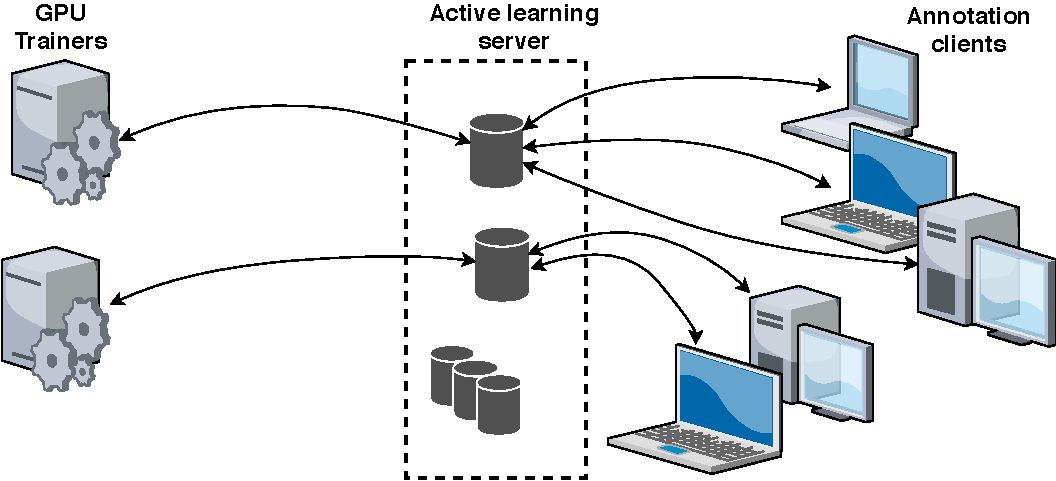
\includegraphics[width=1.0\linewidth]{annotation/connectivity.pdf}
  \caption{Connectivity of the annotation system}  
  \label{fig:connectivity}
\end{figure}

The system can be broken down into three parts running separately but communicating with each other (see figure~\ref{fig:connectivity}). The server sits in the middle and communicates with both trainers and clients, as well as storing data (image data, annotations and annotation history, trained models and annotations).

The main reason for splitting the server and trainer was initially for practical reasons with the client and server both written in \gls{GHC} Haskell, and the deep learning framework of choice being Pytorch \cite{Paszke2017}. The server and client are written in Haskell, the former running naively, the latter compiled to JavaScript using \gls{GHCJS}. The interface uses a \gls{SVG} for display, but in future I plan to switch to \gls{HTML} canvas for faster rendering in a wider variety of browsers, and resolve issues with displaying hundreds of annotations at once.

Splitting server and trainer also provides some advantages. It allows the server to act as a portal through which users can work on several datasets. One or many trainers can be shared concurrently or time shared without having to run new instances of the server. 

The current reality is more simple, a single trainer services the server and operates on a first come first served basis. One dataset at a time is trained, until a period of inactivity (no images submitted for $ n $ training epochs). A trainer still services clients working on inactive datasets by providing detection (best models for each dataset are kept in \gls{CPU} memory), but trains on only one dataset at a time. 

Due to the nature of memory management on a \gls{GPU}, and the memory requirements of training, I interleave requests originating from clients and training. When a user selects an image, the first action taken is to query the trainer for a set of detections. It is therefore necessary to stop training temporarily, run object detection inference on the image in question, and then resume training. In an attempt to mitigate the delay, a small number of frames are processed in advance according to the current image selection policy in use at the time. For larger images, the transmission and decoding of image data in the current system causes more significant visible delay than the response time to the object detection query.

In future, it would be an advantage to allow one or more \gls{GPU} processes to be dedicated to serving user requests, in the interests of reducing response time. Low response time is important especially for the purposes of interacting with video if skipping forwards and backwards in time (spanning potentially many frames at a time), so this can occur without unreasonable delay.

\begin{figure}[h!]
  \centering
  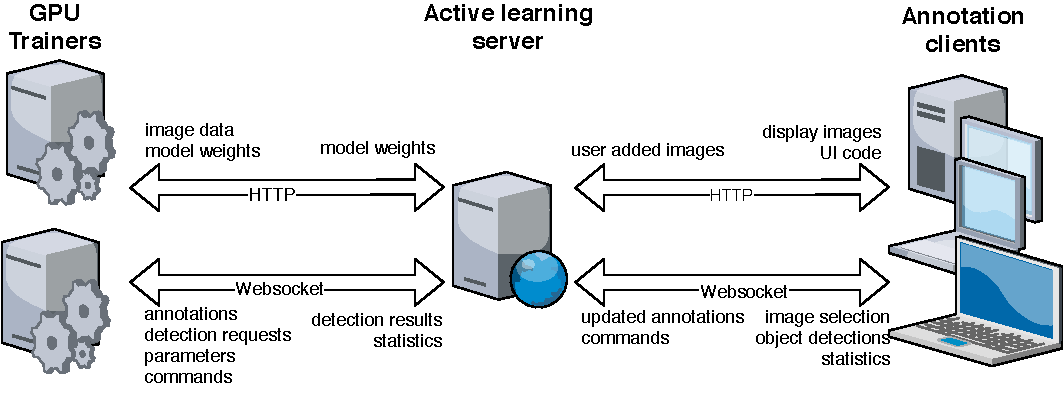
\includegraphics[width=1.0\linewidth]{annotation/data_flow.pdf}
  \caption{Data flow between services for the annotation system}  
  \label{fig:data_flow}
\end{figure}

An illustration of the data flow which occurs between different parties can be seen in figure~\ref{fig:data_flow}. Large binary data is shared using \gls{HTTP}, for example model weights and images are distributed this way. Other data is communicated over websocket connections using \gls{JSON} text. Examples of this include synchronising new annotations and image statistics, which are continually updated to the client for the purpose of the example selection in active learning.

Image data is stored on the server and transmitted as required to the trainer and the client. Images are sent to the client for viewing and inspection, and to the trainer for training and cached for more efficient loading. 

Models are stored on the server and requested by the trainer as required, for example when starting training on a dataset, the trainer requests the previously stored model weights. The trainer also caches copies of weights (as required) of recently used models for the purposes of inference as required by the client for every image opened. Given the large size of data involved in transmitting large images, and also updating model weights, it is important for the server to have a fast connection to the trainer.

\subsection {User interface}

I provide a web interface for the following reasons:

\begin{enumerate}
    \item Easy distribution
\end{enumerate}
Any system with a web browser can be used as a client. A web interface sidesteps difficulties with hardware requirements (a modern \gls{GPU}) and difficult to install software dependencies typically required to run \gls{CNN}s at a reasonable speed.
\begin{enumerate}[resume]
    \item Local GPU not required
\end{enumerate}
By running the trainer on another system, anyone can use the system without requiring a local GPU. One of the problems with usability, from my earlier work, was that GPU intensive tasks running on the same computer ruin the responsiveness of a user interface. To my knowledge, there is no good way to run a heavy \gls{GPU} intensive processing task at a low priority so that the user interface remains responsive.
\begin{enumerate}[resume]
    \item Enables collaborative annotation/crowd sourcing
\end{enumerate}
A web interface enables a straightforward extension to use for larger scale annotation with multiple users annotating the same dataset. An example can be seen in~\ref{fig:connectivity}, showing two groups of users operating on the same datasets.


The trade-off for a web interface is in performance, as it prevents doing computationally heavy calculation on the client side, especially for loading and processing large images. For this work, we face no such difficulty, though for example, a superpixel based tool for mask annotation would be more challenging. With newer web technologies such as WebAssembly \cite{Haas2017}, it is possible to run code at near native speeds in a browser and WebGL shaders for GPU programming.



\section{Future Directions}
\label{sec:design_future_direction}

\subsection {Removal of thresholds}
In the future, a lot of attention will be on making the annotation process more streamlined with less manual intervention required. Determining thresholds more automatically, or automated calibration using validation will be a focus.

\subsection {Improve rendering efficiency}
The user interface will switch rendering to a canvas based renderer from the current SVG rendering. This is needed to run on a wider variety of browser, and improve performance for situations where hundreds or thousands of annotations are present on a single image.

\subsection {Restricted annotation interface}
Splitting the user interface into an annotation interface and a supervisory interface will be necessary to support multi-user annotation. The annotation interface will be purely for annotation and has few settings, whereas the supervisory interface is much like the current interface, with full control over the process and with the ability to monitor others.

\subsection {Deployment on cloud services}
Currently, setting up a server and training processes is a manual job, and although it is simple to access through the web interface once setup, more general usage will be enabled through providing scripts to deploy the software (along with images) to cloud services such as \gls{AWS}. 

\subsection {Exposing parameters and settings}
 Many object detection model and training settings in the current implementation are still stored the training process and not controlled centrally. It is planned to expose those parameters through the user interface, and importantly, be able to adapt to those training parameters (even if it requires restarting the training).

\subsection{Visualisations and metrics in the interface}

The current approach to providing metrics to a user, is to run an instance of Tensorboard next to the training process. However, an alternative solution will be sought which means logs can be stored with the rest of the data (rather than stored as Tensorboard logs by the training process).



% \setcounter{chapter}{5}
% \chapter{Object~Detection}
\label{chap:object_detection} 

\section{Introduction}

In this chapter I describe the object detector, training and evaluation metrics used in the object detection annotation system described in chapter \ref{chap:design} and used in this thesis. I describe the object detector, and describe the key differences and the motivations behind those differences in adapting this object detector for the purposes of assisting annotation.

The object detector is based off a single-shot \gls{CNN} detector called RetinaNet \cite{Lin2017}, which was selected for it's simplicity and efficiency, while having close to state of the art accuracy. The major differences from the method in \cite{Lin2017} and brief motivations for each are:

\begin{itemize}
    \item Shared weights between classification sub-networks at different pyramid levels. This was found to make training much faster at the beginning.
    \item No normalisation of the loss function (by number of anchor matches), in order to accommodate images with no positive annotations.
    \item Training on crops of high resolution images, but evaluation on complete images.
    \item Use of cyclical learning rates in training, to accommodate incremental additions to the training set.
\end{itemize}

Each described in more detail later in this chapter. After describing the details of the object detector we test some of the hypotheses which led us to these decisions (as well as another, relating to image annotation in general):

\begin{itemize}
    \item {It is possible to train object detectors at high resolution using only cropped sections; and keeping images at high resolution will provide more accurate object detection}
    \item {When training a single class object detector it will learn faster than multi-class object detectors}
    \item {When incrementally adding images through annotation; training the object detector will adapt to new examples better when using a cyclical learning rates}
\end{itemize} 

\section {Image preparation}

One thing which was noticed in the implementation of the segmentation tool from chapter \ref{chap:bootstrap} was that the original images were often much clearer than the scaled down images for a human annotator to see fine details which can be lost at lower resolution. It is not necessary to train the object detector on the same resolution as seen by a human annotator, but if a human annotator can't see important details, it would seem likely to make the task much more difficult for machine model, as well.

With that in mind I focused on preserving resolution for the annotation process. High resolution images present a cost in terms of training (and inference) time, also in terms of memory and data storage and data transfer over a network, all of which make smaller images preferable. In section \ref{sec:scale_crop} I experimentally validate this idea, comparing training with different resolutions (and crop sizes) for a selection of datasets.

The additional benefit to preserving resolution is that performance of a given object detector has generally been shown to be better with higher image resolution, when training on data with a limited number of classes, we hypothesis that it is possible to get away with larger image sizes by using smaller crops of the original images to train, as long as the objects fit in the image crops. We do some experiments on this idea in section-\ref{sec:validation}, in order to verify these assumptions.

As a counter example the images in the PASCAL VOC \cite{Everingham2008}, or COCO\cite{Lin2014} datasets have a large range of scales, distributed much more evenly with large objects occupying large portions of the image. For the majority of data experimented on in this thesis, the objects of interest occupy an area much smaller than the whole image size. An analysis of object sizes of two of the less extreme datasets compared to VOC and COCO can be seen in figure \ref{fig:box_sizes}.


\begin{figure}[ht]
\centering
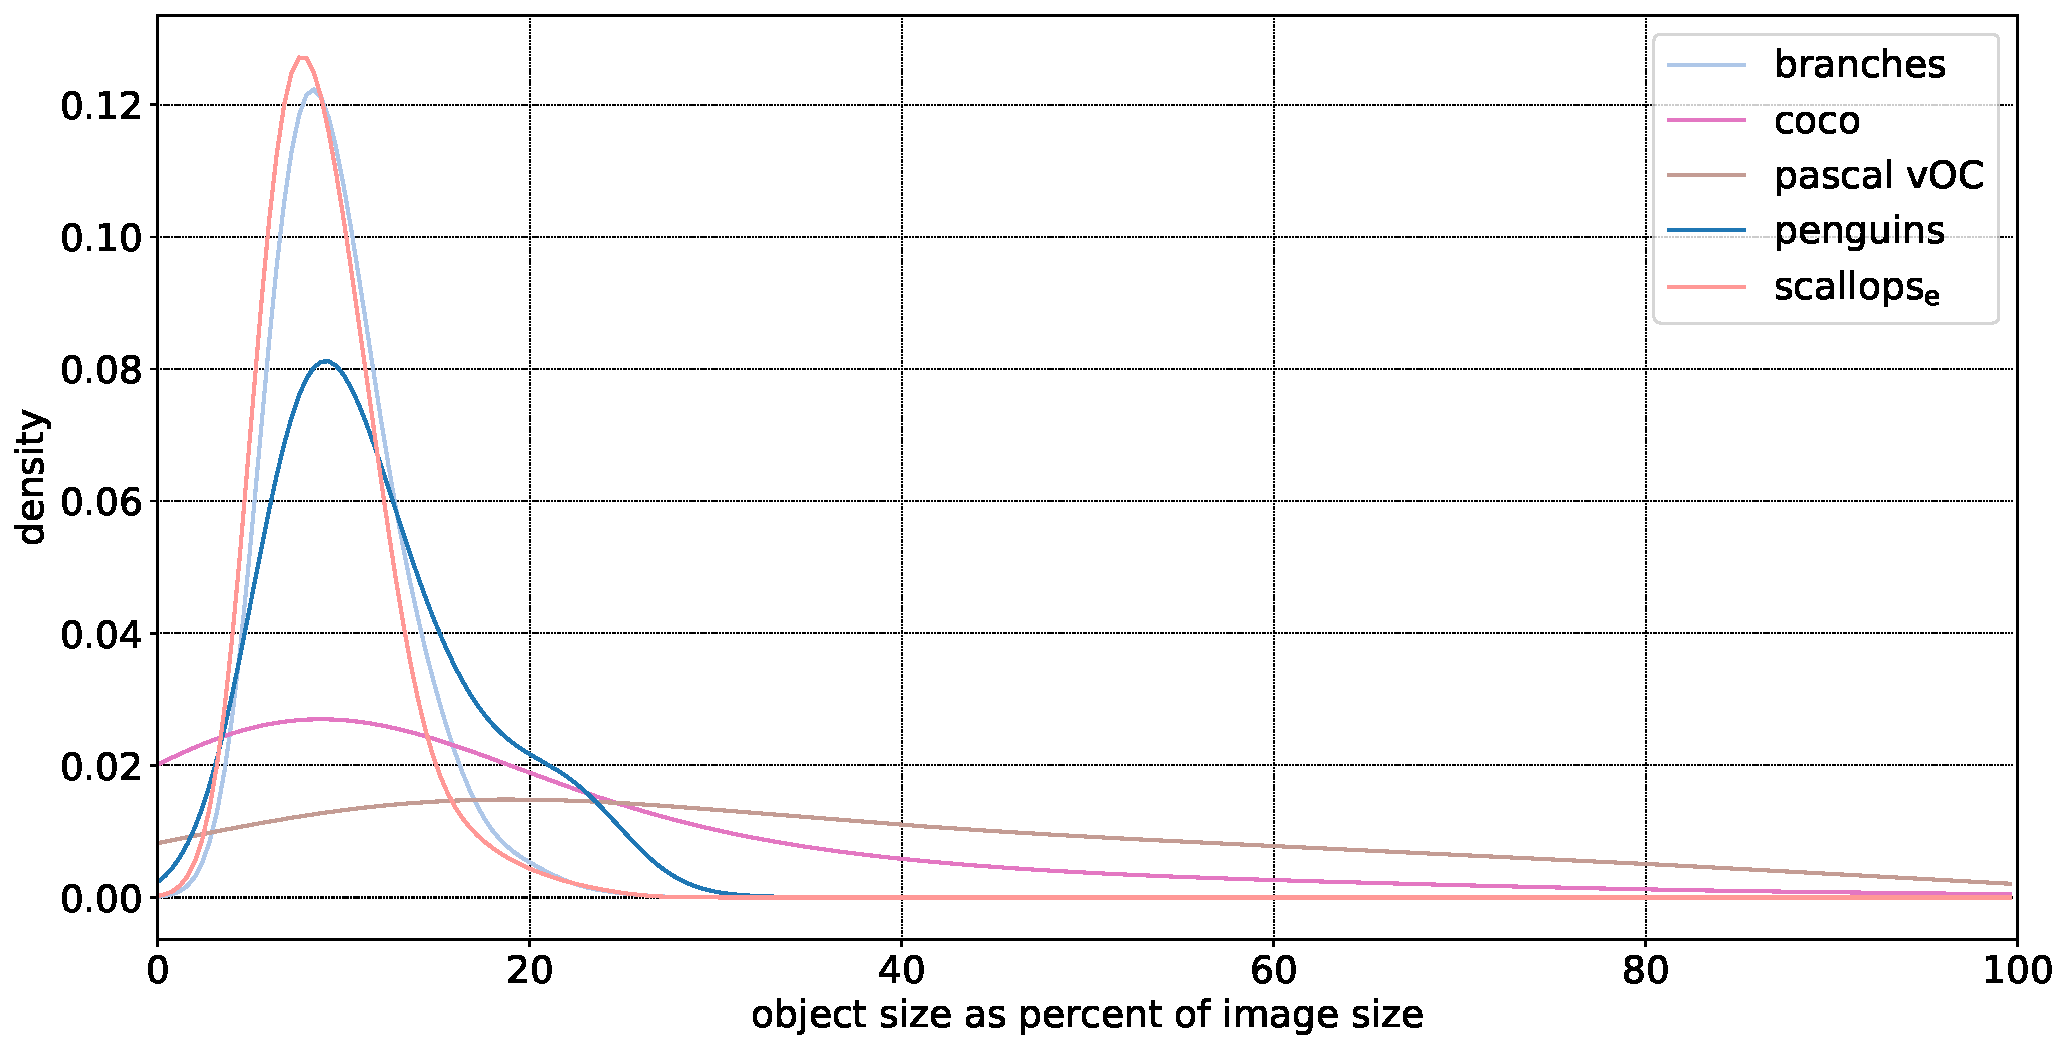
\includegraphics[width=0.9\linewidth]{charts/summaries/sizes_density.pdf}
\caption{Object bounding box size distributions as percent object to image size (average of width and height ratios) }
\label{fig:box_sizes}
\end{figure}


Use of simpler, faster models has been successful as the backbone of the object detection network (for example ResNet--18), which enables larger images in both training and evaluation. Time taken for evaluation and training is also much improved relative to using larger networks. For the smaller datasets in our experiments I did not see large improvements in accuracy when using larger backbone networks.

\begin{table}[h]
  \centering
    \caption{Ranges of parameters used for image augmentation, translation occurs as part of a cropping process}
    
  \begin{tabular}{ l  l }
    Parameter & Range \\
    \toprule
    scale (log uniform) & ${3/4}$--${4/3}$  \\ 
    aspect scale  & $ 1 \pm 0.1 $  \\ 

    brightness adjustment (additive) & $ \pm 10 $ \\ 
    contrast (multiplicative) & $ 1 \pm 0.1 $ \\ 

    gamma adjustment & $ \pm 0.1 $ \\ 

    hue shift & $ \pm 5 $ \\ 
    saturation shift & $ \pm 5 $ \\ 
    
    horizontal flips & $ P = 0.5 $ \\ 
    
    \bottomrule
  \end{tabular}
\label{fig:obj_augmentation}
\end{table}

After applying augmentation (photo-metric distortion and scaling) with parameters described in table \ref{fig:obj_augmentation} and image whitening (described below), a region is cropped from the resulting image at random. In the case where the crop region is larger than the input image, an image is created with pixels set to zero and the input image is placed at a random position within the image.

The crop sizes used in experiments, and in image annotation are specific to each dataset, ranging from $1024\times1024$ for the \emph{apples1} and \emph{apples2} datasets, down to $320\times320$ for the \emph{branches} dataset.

We employ image whitening to ensure consistency with ImageNet trained models (used as the backbone of the networks) subtracting mean (r, g, b) $ (0.485. 0.456, 0.406) $ and dividing by standard deviation $ (0.229, 0.224, 0.225) $.


\section {Object detection}

The object detection method I have been using for the following experiments is a modified RetinaNet \cite{Lin2017} as a strong near-state of the art object detector with a simple implementation. RetinaNet is a type of single shot object detector, meaning that it detects all objects together in one pass, as opposed to two stage detectors which first identify sets of bounding box proposals and then have a second pass to refine those box proposals into concrete detections. Single shot detectors (such as \gls{SSD} \cite{Liu2016a} or RetinaNet) typically achieve faster inference and training time by skipping the second refinement phase, at a slight cost of accuracy.  

Many object detection methods are based on sliding windows, where windows of fixed sizes are moved across an image and attempt to match objects of that size at each position. \gls{CNN} based object detectors achieve this using anchor boxes, where the sliding window is replaced by a simultaneous matching of boxes at each point across an image. Using a fixed set of anchor boxes limits the localisation accuracy, so the counter point to matching anchor boxes is also estimating a transformation to refine an anchor box to fit the more specific size of the object.

RetinaNet is based off Feature Pyramid Networks \cite{Lin2017a} which uses feature maps produced at multiple levels of a \gls{CNN} to classify anchor boxes of different sizes, where many smaller anchor boxes match smaller objects on higher resolution feature maps and fewer larger anchor boxes match larger objects. 

The object detection models bear close similarly to the segmentation models discussed and used in chapter \ref{chap:bootstrap}, such as UNet \cite{Ronneberger2015}. \gls{FPN} models utilise shortcut connections in the same way, the major difference from segmentation models is that anchor boxes are predicted at multiple levels, where segmentation models output mask predictions only at one resolution.


\subsection {Network architecture}
\label{sec:architecture}

Some parameters and network architectures differ from the original paper. For the most part the modifications are small things which seem to enable it to learn better on the kind of small datasets used for experiments in this work. 

These include adding extra residual layers to the decoder, shown in figure \ref{fig:detection_network}. It is more similar to the network shown in  \ref{chap:bootstrap} than the \gls{FCN} network. A key difference is that neither the weights between classification sub-networks nor box regression subnets are shared between different scales  (the original shares weights between classification sub-networks). Shared weights were found it to slow down initial training considerably in the initial phase. 

Other differences are necessary to accommodate different box sizes (usually using additional prediction outputs from earlier layers with finer anchor boxes to handle small objects).

\begin{figure}[h]
  \centering
  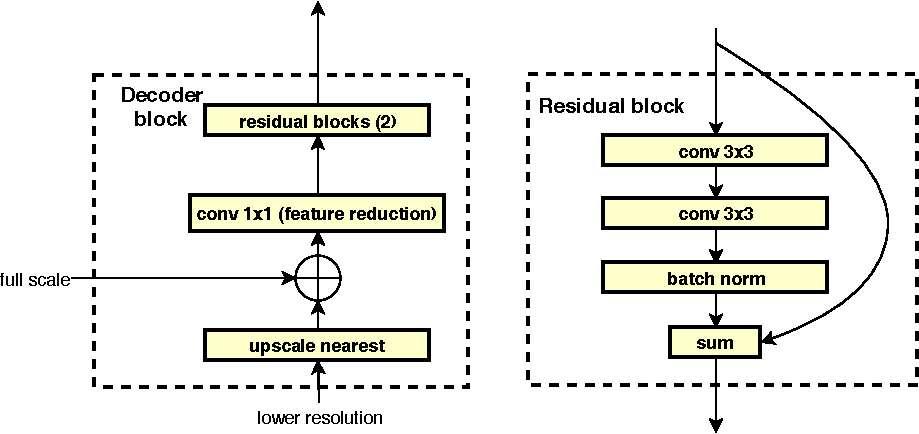
\includegraphics[width=1.0\linewidth]{figures/annotation/decoder_block.pdf}
  \caption{Decoder block, responsible for merging half resolution features with features from full resolution skip connections }  
  \label{fig:decoder_block}
\end{figure}


\begin{figure}[h]
  \centering
  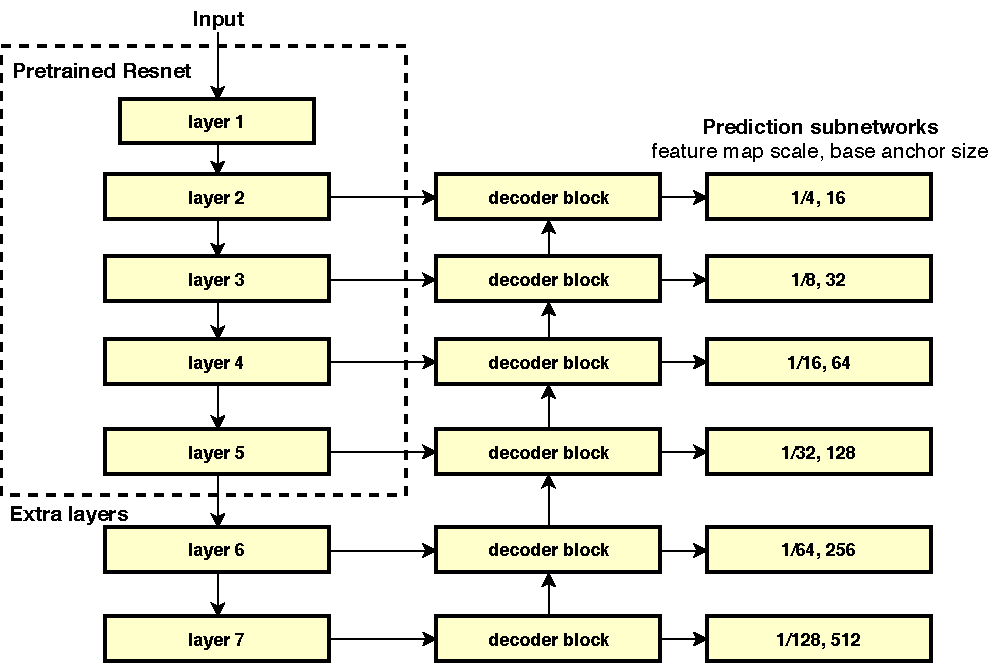
\includegraphics[width=1.0\linewidth]{figures/annotation/detection_network.pdf}
  \caption{Object detection network, built on the backbone ResNet }  
  \label{fig:detection_network}
\end{figure}

\begin{figure}
  \centering
  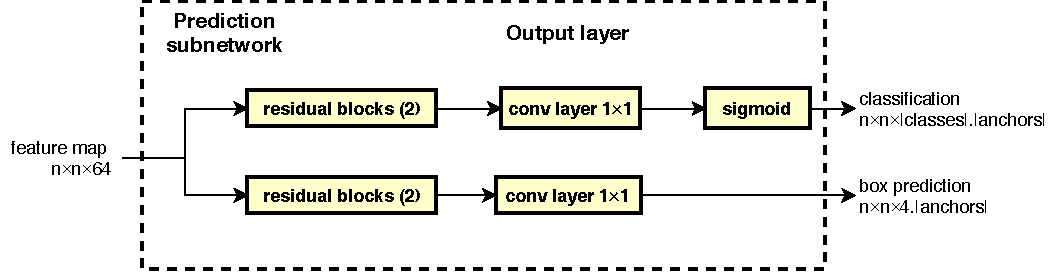
\includegraphics[width=1.0\linewidth]{figures/annotation/prediction_subnet.pdf}
  \caption{Prediction sub-network with two streams, one for classifying anchor boxes with one output per class for each anchor box, the other stream for location regression for each anchor box (shared between classes)}    
  \label{fig:prediction_subnet}  
\end{figure}

\subsection{Initialisation}

Using the initialisation in \cite{Lin2017} where all new convolutions added to the backbone are initialised with $\sigma=0.1$ (and no bias). The final layer of the classification sub-network has bias initialised to $b = −log((1 − \pi)/\pi) $ whereby at the start of training every anchor box is assigned confidence of $~\pi$, we use $\pi=0.01$. With this initialisation the network becomes robust to a wide range of resolutions and learning rates.


\subsection{Anchor boxes}

\begin{figure}
  \centering
  \begin{subfigure}[t]{0.33\textwidth}
  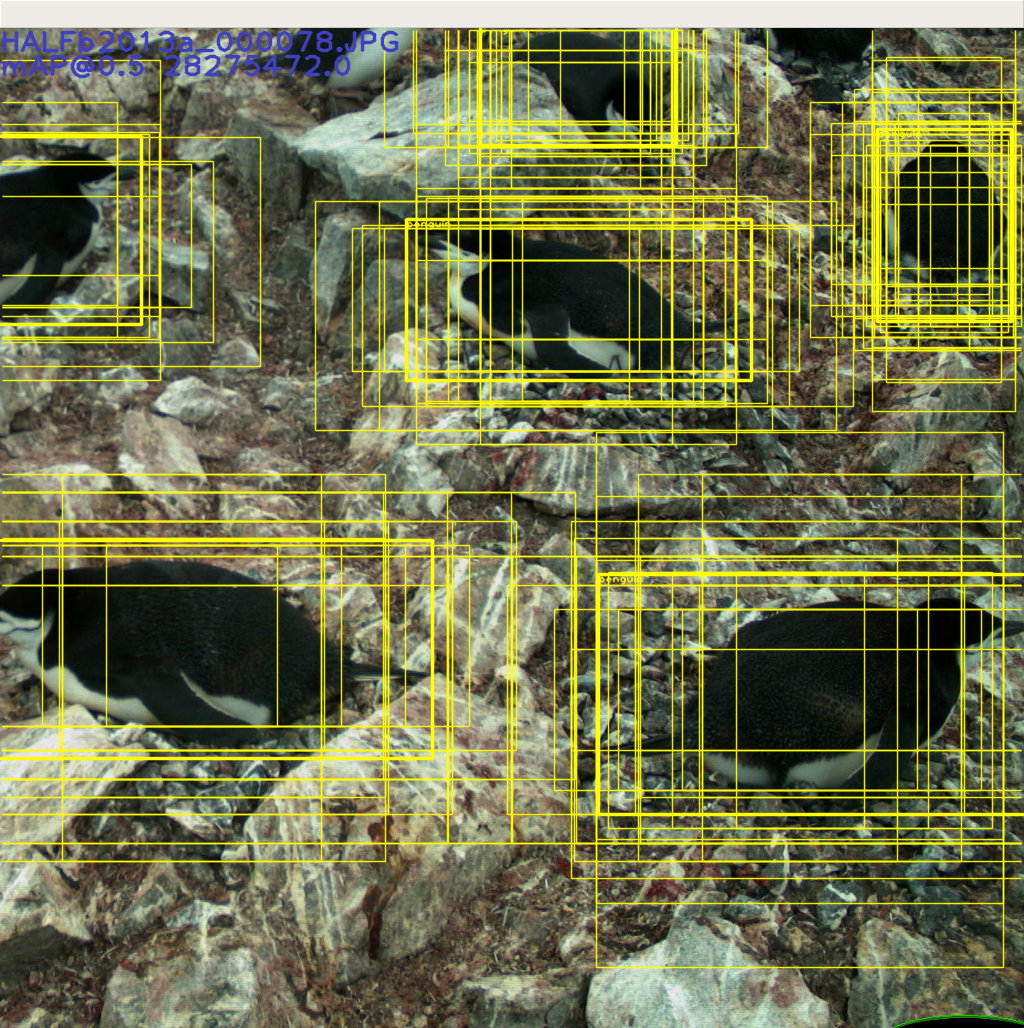
\includegraphics[width=0.95\linewidth]{figures/object/anchors.png}
  \caption{Anchor boxes from class predictions}
  \end{subfigure}%
  \begin{subfigure}[t]{0.33\textwidth}
  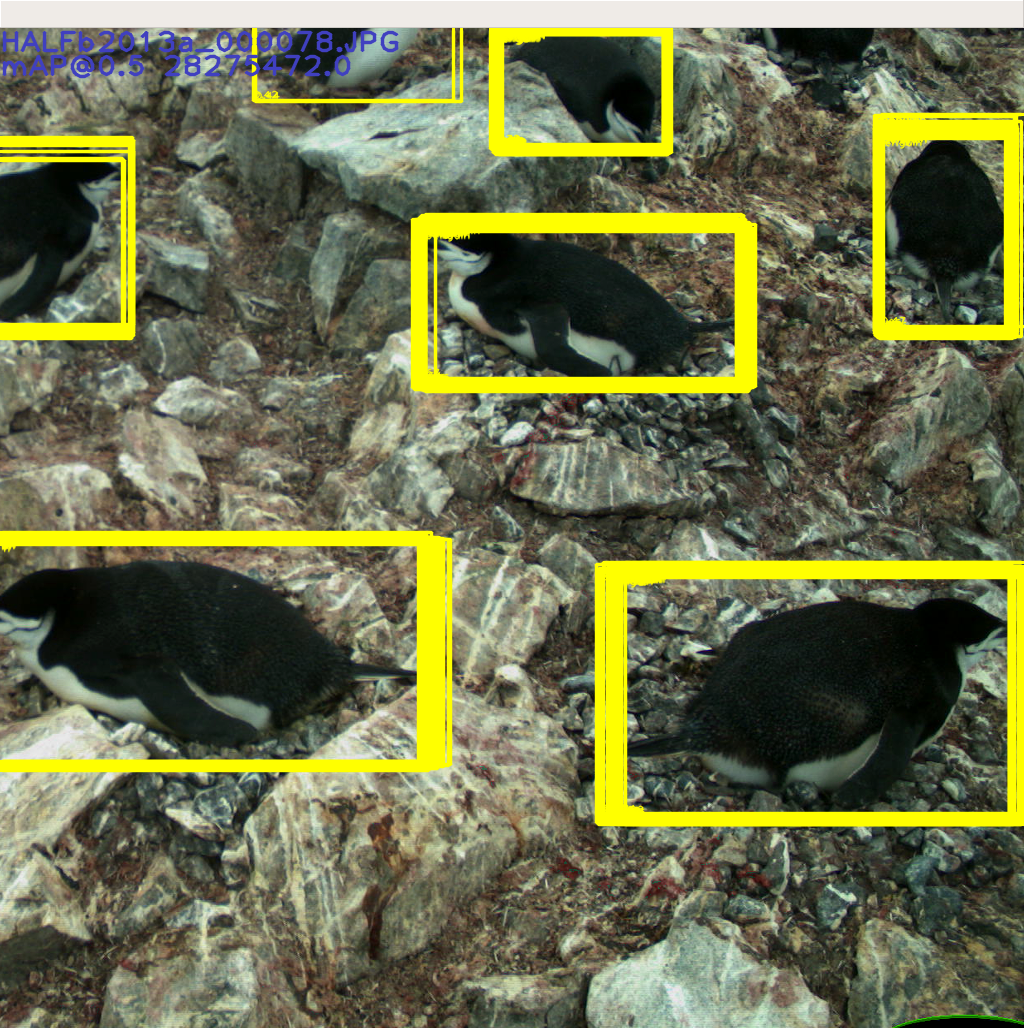
\includegraphics[width=0.95\linewidth]{figures/object/predictions.png}
  \caption{Refined anchor boxes after transformation}
  \end{subfigure}%
  \begin{subfigure}[t]{0.35\textwidth}
  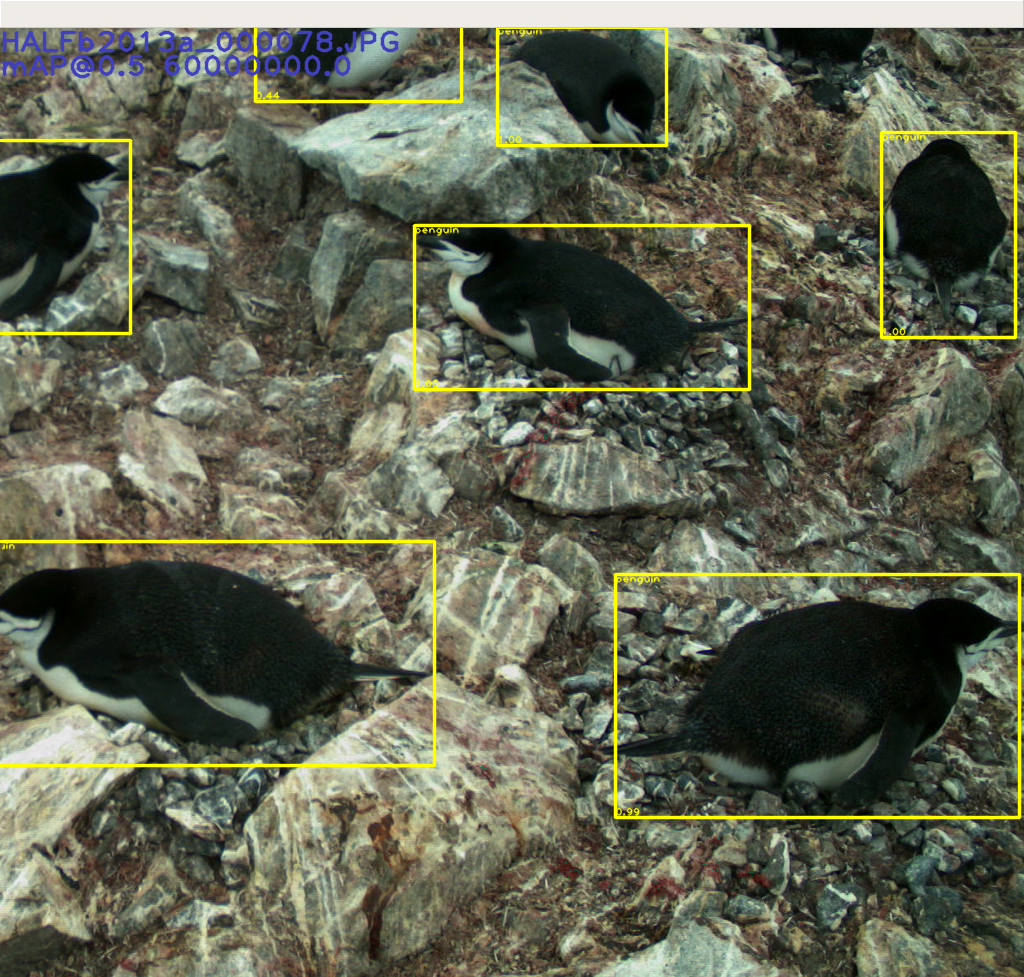
\includegraphics[width=0.95\linewidth]{figures/object/final.png}
  \caption{Final predictions after Non Maxima Suppression}
  \end{subfigure}%  
  \caption{Illustration of the stages of box prediction and refinement process}
  \label{fig:anchor_boxes}
\end{figure}


We use translation invariant anchor boxes as per \cite{Wang2017}, anchor boxes are the set of default locations and box sizes for which the \gls{CNN} can predict if and which object exists. It is unfeasible to provide a discrete set of boxes large enough to cover all possible object locations, therefore each anchor box is also modified by a scale and translation (details below in section \ref{sec:regression}) to fine tune anchor boxes to fit objects in the image.

Set of anchors boxes are used for each level with aspect ratios $ \in \{0.5, 1, 2\} $ and scales $ \in \{2^0, 2^{1/3}, 2^{2/3}\} $. For each feature map at level $k$, with a base scale of $ 2^{k + 2} $ pixels, the set of 9 anchor boxes (all combinations of aspect and scale) are tiled centred on each feature map pixel. 

In the case of counting, where circles are used for annotation only three anchor boxes are used, only the square aspect ratio is used at the same three scales. For all intents and purposes the circles with radius $r$ are treated as a square box with side lengths $2r$, and the box regression sub-network modified to produce only $3$ outputs (enforcing square aspect ratio for height and width).

Feature maps on levels $3$--$7$ are used for most datasets giving the smallest (square) anchor at $32\times32$ and the largest at $812\times812$. In the case of datasets with very small objects (for example, aerial penguin counting and wide angle counting of seals) we add in anchor boxes on level 2 which allow for objects as small as $16 \times 16$.

For those with smaller objects such as the aerial Adellie penguin counting, the tree branch detection and the seal counting an extra feature map is used giving anchor boxes as small as $16\times16$ and more densely tiled.

In training, anchor boxes are selected by matching on \gls{IOU} overlap with ground truth boxes. Each anchor is matched with the ground truth box with highest overlap. An anchor box matches a ground truth box as a positive if $ IoU >= 0.5 $, anchors with $ IoU < 0.4 $ are treated as negative, and those boxes with $ 0.5 > IoU >= 0.4 $ are ignored (omitted from either positive or negative for computing loss).

Ground truth boxes will match with potentially many anchor boxes, but those in close proximity and similar size may mean that boxes which would have otherwise matched do not, because anchors cannot be assigned to more than one ground truth.

\subsection{Total loss function}

The total loss function is defined as a balanced sum between box regression ($L_{loc}$) and class prediction loss ($L_{class}$). 

\begin{equation}
L  = L_{loc} + \lambda L_{class}
\label{eq:loss_total}
\end{equation}

\subsection {Box regression loss}
\label{sec:regression}


We use the anchor box encoding used in \gls{RCNN} \cite{Wang2017} for the purpose of calculating location loss. The loss is a smooth-L1 loss over regression target ($t^*_x, t^*_y, t^*_w, t^*_h \in t^*_i$) giving a transformation from an anchor box ($a_x, a_y, a_w, a_h$)  to a set of regression targets $t^*_i$ from the ground truth ($g_x, g_y, g_w, g_h$). 

The boxes are encoded as the offset of the centre in both directions (in proportion to the box size) and the log scale of height and width. The encoding of the four targets are given as:

\begin{equation}
\begin{split}
t^*_x = (g_x - a_x) a_w\\
t^*_y = (g_y - a_y) a_h\\
t^*_w = log(g_w / a_w)\\
t^*_h = log(g_h / a_h)\\
\end{split}
\label{eq:encoding_rcnn}
\end{equation}

The localisation loss can be directly computed from these targets and the output of the box prediction sub-network as the sum smooth-L1 regression of $t_i^* - t_i$. Smooth-L1 is a combination of L2 loss near the origin and L1 loss otherwise. It is given as:

\begin{equation}
L_{1;smooth} = 
\begin{cases*}
|x| & if $|x|>\alpha $ \\
\frac{1}{|\alpha|}x^2 & if $|x| \leq \alpha$
\end{cases*}
\label{eq:smooth_l1}
\end{equation}

The commonly used value $\alpha = 0.5$ is used here. The total localisation loss is then summed across matching (\gls{IOU} > 0.5) anchor truth boxes as:

\begin{equation}
L_{loc} = \sum_i{L_{1;smooth}(t_i^* - t_i)}
\label{eq:loss_loc}
\end{equation}

By rearranging the equations we can then do the reverse process and decode bounding boxes from box predictions $t_x, t_y, t_w, t_h$  and an anchor box. These predictions are then in units of pixels and given as the predictions of the object detection network (after a \gls{NMS} process to cull duplicates).

\begin{equation}
\begin{split}
p_x = a_x + t_x  a_w\\
p_y = a_y + t_y  a_h\\
p_w = exp(t_w) a_w \\
p_h = exp(t_h) a_h\\
\end{split}
\label{eq:decoding_rcnn}
\end{equation}

\subsection {Classification loss}
\label{sec:loss}

The experiments use a modified version of the Focal Loss \cite{Lin2017} to handle the class imbalance (negative vs. positive) present when sampling anchor box predictions densely.

Focal Loss \cite{Lin2017} re-weights the standard \gls{BCE} loss function to deal with a large number of easy negative examples in object detection (the number of unmatched anchor boxes greatly outnumbers the number of matched anchor boxes). Focal Loss enables dense sampling of negative examples present in an image. The standard approach in to dealing with the imbalance between positive and negative examples has been to sample the most significant negative examples to provide a certain positive to negative ratio.

As defined \cite{Lin2017}, we use the same terminology and variable naming for consistency. The basic two class \gls{CE} equation for binary prediction from the model classifier $p \in \left[0, 1\right]$, and label $y \in \{0, 1\}$  is given:

\begin{equation}
CE(p, y) = 
  \begin{cases*}
  -log(p) & if $y = 1$\\
  -log(1-p) & otherwise\\
  \end{cases*}
\label{eq:cross_entropy}
\end{equation}


The cross entropy can be rewritten by defining $p_t$ the prediction relative to the given label.

\begin{equation}
p_t = 
  \begin{cases*}
  p & if $y = 1$\\
  1 - p & otherwise\\
  \end{cases*}
\label{eq:class_prob}
\end{equation}

Allowing the \gls{CE} equation to be rewritten more simply:

\begin{equation}
CE(p_t) = -log(p_t)
\label{eq:short_cross_entropy}
\end{equation}


In order to deal with class imbalance the key idea of \cite{Lin2017} was to re-weight the classification loss to be smaller for well classified boxes (small $p_t$) and to be relatively much larger for badly classified boxes (large $p_t$). This was achieved by multiplying the cross entropy by a factor of $(1 - p_t)^\gamma $ with parameter $\gamma$ a sharpening parameter, to give the focal loss:

\begin{equation}
FL(p_t) = - (1 - p_t)^\gamma log(p_t)
\label{eq:focal_loss_p}
\end{equation}

Another way of dealing with class imbalance is to weight one of the classes (in the binary case given here either the positive c

A balanced cross entropy loss can then be written by adding a class weighting $\alpha \in \left[0, 1\right]$ the weight for the positive case in the two class setting, and an analogous $\alpha_t$:

\begin{equation}
\alpha_t = 
  \begin{cases*}
  \alpha & if $y = 1$\\
  1 - \alpha & otherwise\\
  \end{cases*}
\label{eq:balanced_weight}
\end{equation}

Then the balanced, focused, cross entropy is defined:

\begin{equation}
FL(p_t) = -\alpha_t (1 - p_t)^\gamma log(p_t)
\label{eq:focal_loss}
\end{equation}

I adopt the parameters given in \cite{Lin2017}, using $ \gamma = 2 $, and $ \alpha = 0.25 $. 

The total class loss is then given as the sum of the focal loss computed densely across all classes and anchor boxes in the image (except for anchor boxes between positive threshold and negative threshold $0.4 <= IoU < 0.5$ which are ignored). For $K$ classes, $p_i$ is the size $K$ prediction vector from the network for anchor box $i$ and $p^*_i$ is the size $K$ one hot target vector.

\begin{equation}
\begin{split}
L_{class} = \sum_i{\sum_{k \in K}FL(p_{ik}, p^*_{ik})}
\end{split}
\label{eq:class_loss}
\end{equation}

\subsection {Learning rate and Normalisation}

In \cite{Lin2017} a normalisation occurs over the total loss by the total number of positive matching anchor boxes, in order to average the error from the positive targets (making an assumption that the negative targets contribute a negligible amount to the total loss). As the datasets used in this work often don't contain any positive ground truth boxes it was necessary to avoid a division by zero. One method is to add a constant (representing the contribution of the negative classification targets) to the normalisation factor, the other is to divide by a constant value (essentially using a lower learning rate). I experimented a little with both options, finding either to be reasonably robust, the experiments in this work use a non normalised class classification loss.

In all experiments in this work (unless specified otherwise), the learning rate is set to $0.001$ and the balance factor $\lambda=2.5$. Total loss is averaged across each mini-batch, and batch sizes of $8$ are used.

\subsection{Inference and Non-maxima suppression}

In training a large set of anchor boxes are trained to classify each object detection (those overlapping each anchor box by $0.5$ or more). For the purposes of inference detecting more than one box for the same object is undesirable, so a greedy \gls{NMS} is used to eliminate multiple detections of the same object. Figure \ref{fig:anchor_boxes} shows the effect of applying a \gls{NMS} on box predictions, (b) shows the regressed predictions where many boxes overlap the same object (c) shows the result of the \gls{NMS}, leaving a single box on each object. In this work a standard \gls{NMS} procedure as per \cite{Wang2017} is used, where boxes are selected from most-confident to least-confident, boxes overlapping lower confidence boxes by more than an \gls{IOU} threshold (in this work $0.5$) are eliminated.

The use of \gls{NMS} has presents some problems in object detectors notably the inability to handle highly overlapping objects well. Objects high overlap by more than $0.5$ are impossible to accurately detect for such a detector. When used for annotating crowded objects the inability of the object detector to accurately predict highly overlapping objects means in some datasets the user spends a lot of time correcting artefacts caused by limitation of the object detector (by no means limited to \gls{NMS}).


\section{Evaluation metrics}
\label{sec:evaluation_metrics}

The most common metric used in object detection is that of \gls{AP}, as popularised by the Pascal VOC challenge \cite{Everingham2008} and later the COCO dataset \cite{Lin2014}. The \gls{AP} is essentially the area under a recall-precision graph for a particular matching threshold and varies from $0$  to $1$. it's major attraction is that it avoids the need for a detection threshold. It provides a single relatively easy to understand metric which measures precision, recall as well as localisation accuracy (for a particular threshold).

Matches are found by a greedy algorithm in each image (similar to that used in \gls{NMS} above) where the predictions are matched against ground truth boxes from a most-confident to lead-confident order. Each prediction matches it's highest overlap ground truth box where the overlap exceeds the \gls{IOU} threshold (amongst ground truth boxes already unmatched). Matches from all images are then merged and sorted by confidence level of the prediction of the match. True-positives ($tp$) and false-positives ($fp$) are found by counting matched and unmatched predictions from high-to-low confidence, false-negatives ($fn$) are determined at each point by subtracting true-positives from the total ground truth count. 

\begin{equation*}
\begin{split}
p_i = \frac{tp_i}{fp_i + tp_i}\\
r_i = \frac{tp_i}{tp_i + fn_i}
\end{split}
\end{equation*}

From there recall ($r$), and precision ($p$) levels can be determined at the confidence level of each prediction. Special cases are added for $r_0=0, p_0=1$ and $p_n=1, r_n=0$, the precision levels are then made monotonic decreasing:

\begin{equation}
\hat{p_i} = \max_{j \in [i..n]}{p_j}
\end{equation}

\gls{AP} can then be calculated by using trapezoid summation:

\begin{equation}
AP = \sum_{i \in [0..n-1]}\frac{\hat{p_i} + \hat{p}_{i + 1}}{2}
\end{equation}



\gls{mAP} is then defined as the mean of \gls{AP} over classes, and is often notated $mAP@IoU$ for a particular matching threshold IoU, for example $mAP@0.5$ is metric used for evaluation for the Pascal VOC \cite{Everingham2008}, but $mAP@0.75$ for example provides a much stricter matching criteria on the allowable localisation error. In this work we are much more interested in the stricter matching criteria, because a match overlap of $0.5$ represents a box which the annotator will need to manually correct.

To produce a single metric taking into account localisation accuracy \cite{Lin2014} defined a metric COCO \gls{AP} as the mean of \gls{mAP} at a series of matching thresholds $ IoU \in [0.5 : 0.05 : 0.95] $, confusingly this mean-\gls{mAP} is termed just \gls{AP}. We follow this convention however, where we use \gls{mAP} and refer to \gls{AP} as the COCO \gls{AP}.

There are downsides to the \gls{mAP} metric. The precision-recall graph created using decreasing confidence considers only the order of detection confidence. This has implications that the level of false positives which occur at lower confidence than the last true-positive are ignored, in addition the margin between confidence levels is ignored, so the sensitivity to change in confidence levels is not taken into account. The threshold on \gls{IOU} overlap also means that all true-positives which meet the localisation threshold are treated equally, matches which match the ground truth perfectly are scored the same as those which meet only the minimum match threshold. Alternatives exist, although arguably not as easy to understand as \gls{mAP}, for example \cite{Oksuz2018} which tries to weight true-positives for localisation accuracy, as well as attempting to provide a way to determine the ideal detection threshold.



\section {Learning schedule}
\label{sec:schedule}

\begin{figure}[h]
  \centering
  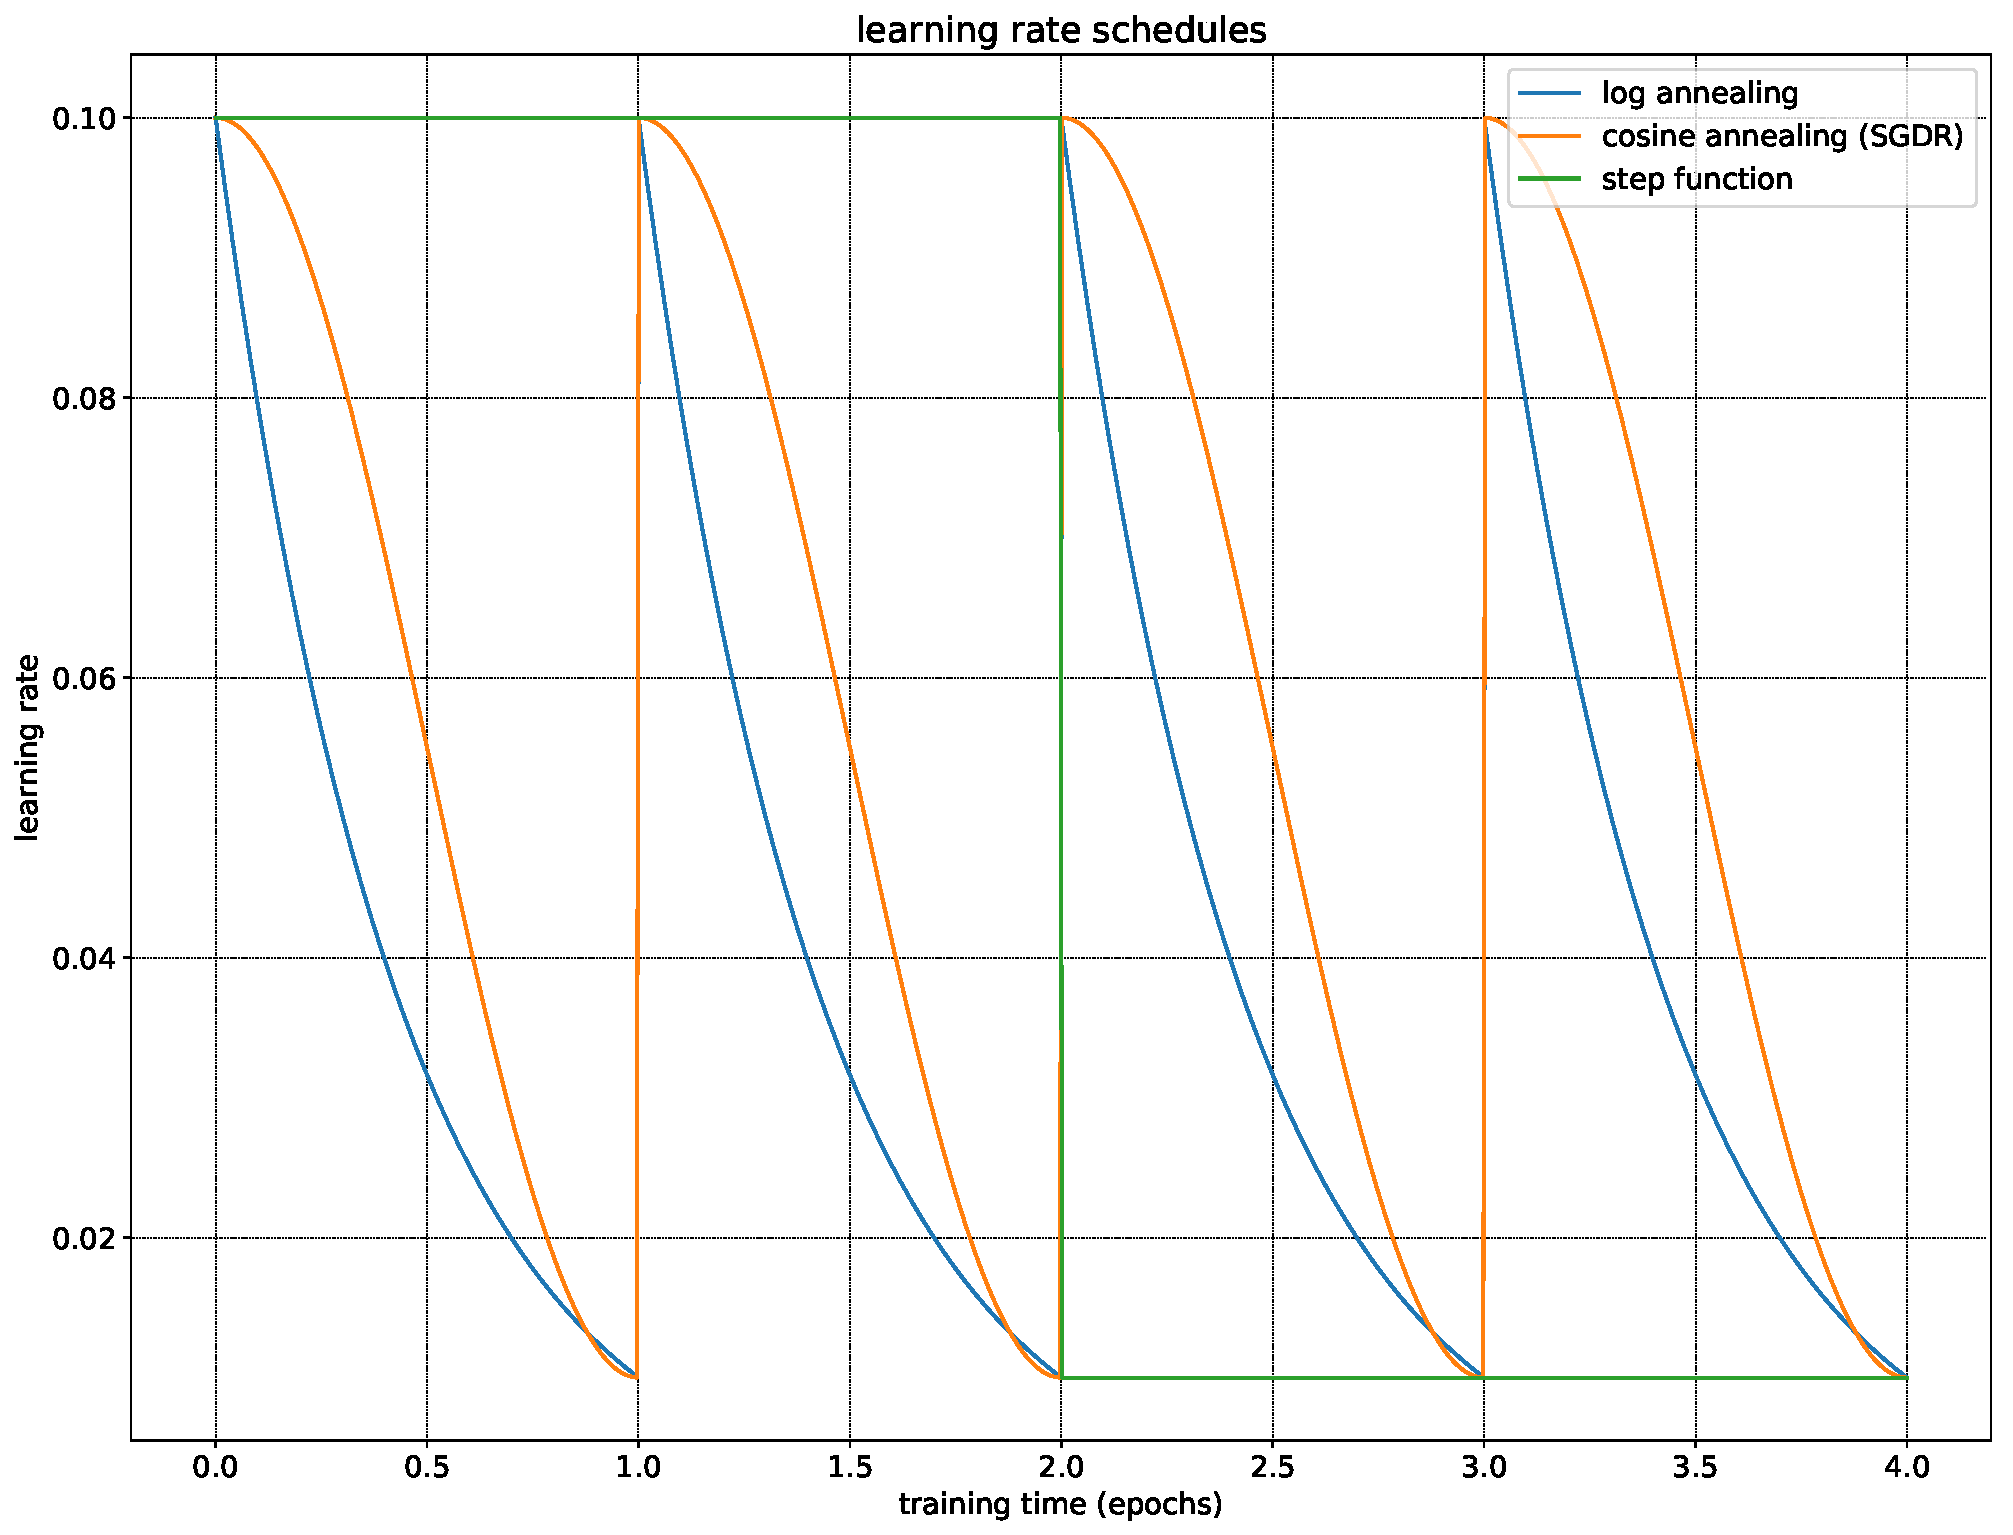
\includegraphics[width=1.0\linewidth]{charts/training/lr_schedules.pdf}
  \caption{Comparison of learning rate schedules, cyclical learning rates and traditional step function.  }  
  \label{fig:lr_schedule}
\end{figure}

In order to facilitate continuous online learning where examples are added over the training lifetime, a cyclical learning rate is used and relatively short learning epochs are used. Epochs are set at a fixed size ($1024$ unless otherwise specified), using a uniform random sampling. Learning rates are set for each batch, reducing over an epoch by a factor of $10$, using a logarithmic annealing shown in equation \ref{eq:log_annealing}. Where $base$ is the base learning rate, and $ t \in [0, 1) $ is the progress across an epoch.

\begin{equation}
annealing_{log}(t) = exp(ln (lr_{min}) (1 - t) + ln(lr_{max})  t)
\label{eq:log_annealing}
\end{equation}

For comparison the learning rate schedule used in \gls{SGDR} \cite{Loshchilov2016}, which has more weight on the highest and lowest learning rates, but otherwise similar.

\begin{equation}
annealing_{cos}(t) = lr_{min} +  \frac{1}{2} (lr_{max} - lr_{min}) (1 + cos (t \pi))
\label{eq:cosine_annealing}
\end{equation}

A comparison of the cyclical learning rates compared to a standard learning rate step schedule is shown for an $8$ epoch training schedule in figure \ref{fig:lr_schedule}.



\section{Methods of inference for high resolution images}
\label{sec:highres_inference}

\begin{figure}[h]
  \centering
  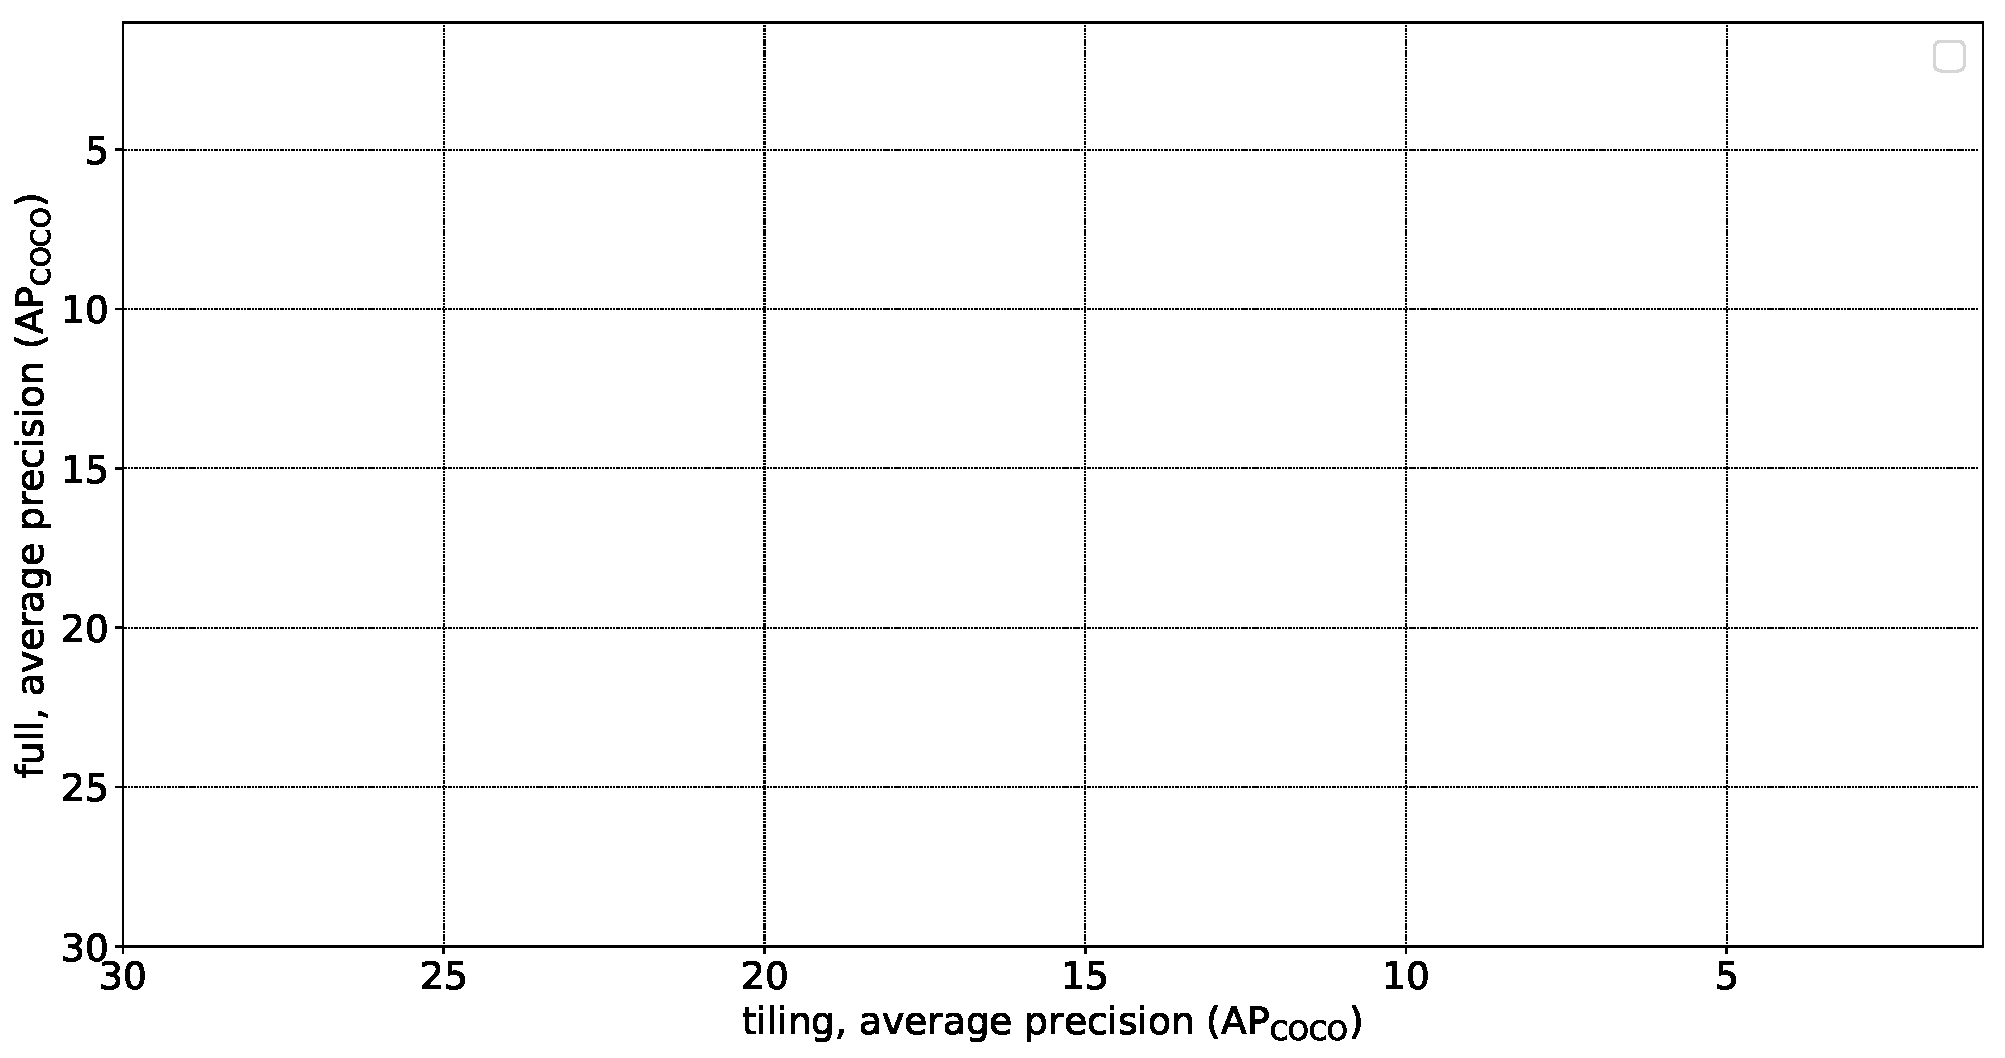
\includegraphics[width=1.0\linewidth]{charts/training/splits_scatters.pdf}
  \caption{Comparison of different inference methods across one training run, inference using tiling vs. inference on full images. Training occurs on crops and evaluating on full images. }  
  \label{fig:inference_method}
\end{figure}

I look at two different possibilities for performing inference on a full resolution image using an object detector network trained only on crops of images; (a) pass in the full image using the property that the network is 'Fully Convolutional', (b) tile images the same size as training crops and collapse the predictions using a combined \gls{NMS}. In order to facilitate this idea the box annotations on the edge of images are estimates of the full bounds of the object; and the anchor boxes are not cropped to the edge of the image.

Object detection networks are flexible and work across a range of input image resolutions. All layers are either convolutions or do not reshape the feature maps (aside from up/down sampling). As a result, passing in a larger image results in a larger output sets at each layer of the pyramid. For an object detection network this corresponds to a larger set of anchor boxes (given that the anchor boxes are translation invariant). The concern is that the up/down sampling behaviour is slightly different for input sizes depending if they're odd or even relative to powers of two. I found this is a legitimate concern, though largely negated if the training crop size is a power of two or a multiple of a power of two.

The second inference method is to tile multiple 'raw' inferences across the full image size using a certain overlap buffer region, the result is sets of overlapping predictions. These overlapping predictions can be decimated using a combined \gls{NMS}, such that it removes duplicates overlapping from two neighbouring tiles. The concern with this method is that edge detections are possibly inaccurate and may produce erroneous predictions which are not removed by \gls{NMS} because of their inaccurate localisation. 

Both methods are tested by testing against the validation set of several different training runs. It can be seen in figure-\ref{fig:inference_method} that both perform very similarly. If there is ever a difference; sometimes one is marginally better, sometimes the other is marginally better, even within the same training run.

\section {Effect of scale and crop size}
\label{sec:scale_crop}

High resolution images present a cost in terms of training (and inference) time, also in terms of memory and data required to transfer over a network. I expect the trade-off to be be worthwhile however. High resolution images are undoubtedly easier to annotate, small details become clear and using down scaled images often makes even the annotation task ambiguous. It is not necessary to feed the model images of the same resolution as the user annotates, but if a human annotator has trouble with ambiguity it seems a reasonable assumption that a \gls{CNN} will also struggle.

Especially for datasets with many small examples, the datasets used here (see chapter for details \ref{chap:7}) contain many small objects, and many objects with a high degree of uncertainty and ambiguity.



The full resolution images do provide the best accuracy, although in many of the datasets half resolution provided almost the same accuracy while providing much faster training and inference. At half resolution an ensemble could be trained in similar time to training one network at full resolution and used to provide uncertainty measurements. On the other hand, as seen below in section-\ref{sec:lr_schedule_exp} the training accuracy is limited by the size of the dataset more than the training time, which is severely dependent on human annotation time which will allow plenty of time for training at high resolution.

Using a larger crop size proved better in three of the four datasets, however for apples it trained faster and achieved roughly the same level of accuracy as the larger crop. Crop size could perhaps be adjusted automatically based on the largest size of the objects.


\section {Learning rate scheduling}
\label{sec:lr_schedule_exp}

I expect cyclical learning rates to much better cope with a stream of new examples provided incrementally, this is important if the model is to provide good assistance to an annotator in a timely fashion. 


\subsection {Single vs. multi-class training}
\label{sec:lr_schedule_exp}

In this experiment I examine the idea that for the purposes of providing annotation assistance, that it is better to focus on a single class, or few classes (from the point of view of training an object detector to aid further annotation). 

\subsection{Single or few-class vs. multi-class}

Given the the experiment in section-\ref{sec:lr_schedule_exp} it is seen that the accuracy of the object detector correlates with the number of examples

With appropriate preparation, annotating a single class at a time should enable a larger number of examples of that class in a shorter period. This is highly dependent on the dataset and the preparation before annotation begins. Some level of pre-sorting or image selection becomes crucial if classes are very sparsely distributed in the input images; for example if there are a lot of classes, but only a hand-full in any particular image.

The datasets used in this work are either single or few-class, with multiple instances per image; with the exception of the \emph{scallops} dataset, where despite being a single class annotation the instances are sparsely distributed amongst the images.







\section{Other factors}

Here I discuss some other factors which had large impact on the performance of the object detection network, but have not been quantified.

\begin{itemize}
    \item {\bf Larger and more sophisticated models}
Primarily we used ResNet-18 \cite{He2015} as the backbone network in all the experiments, there are many larger more sophisticated networks, of the networks used to classify ImageNet ResNet-16 is one of the simplest. Other networks work at least equally as well, but I did not find significant improvement at the expense of slower training and evaluation.
    \item {\bf Shared weights in class prediction sub-network}
RetinaNet \cite{Lin2017} used shared weights for it's class prediction sub-network (figure \ref{fig:prediction_subnet}) at different resolution outputs (but not between box localisation sub-networks). I found in the small scale datasets used in this work that shared weights on the class sub-network significantly slows initial learning. Extra residual layers in the decoder side of the network (figure \ref{fig:decoder_block}) improved this significantly, but not entirely.

\end{itemize}

\section {Conclusion}

This chapter described the object detector used behind the annotation tool, parameters used, methods of training and described some of the rationale for the differences with published literature. Chapter-\label{chap:annotation} attempts to evaluate the annotation software as a whole through it's practical use in annotating several datasets. Some of those datasets annotated this way I have then used to evaluate some of the assumptions used in the design, and the parameter set used in this chapter. 




\setcounter{chapter}{6}
\chapter{Verification Based Annotation in the Wild, Applications to Real World Datasets and Counting Wildlife}
\label{chap:annotation} 

\begin{figure}[htbp]
\centering
\begin{subfigure}[t]{0.24\linewidth}
  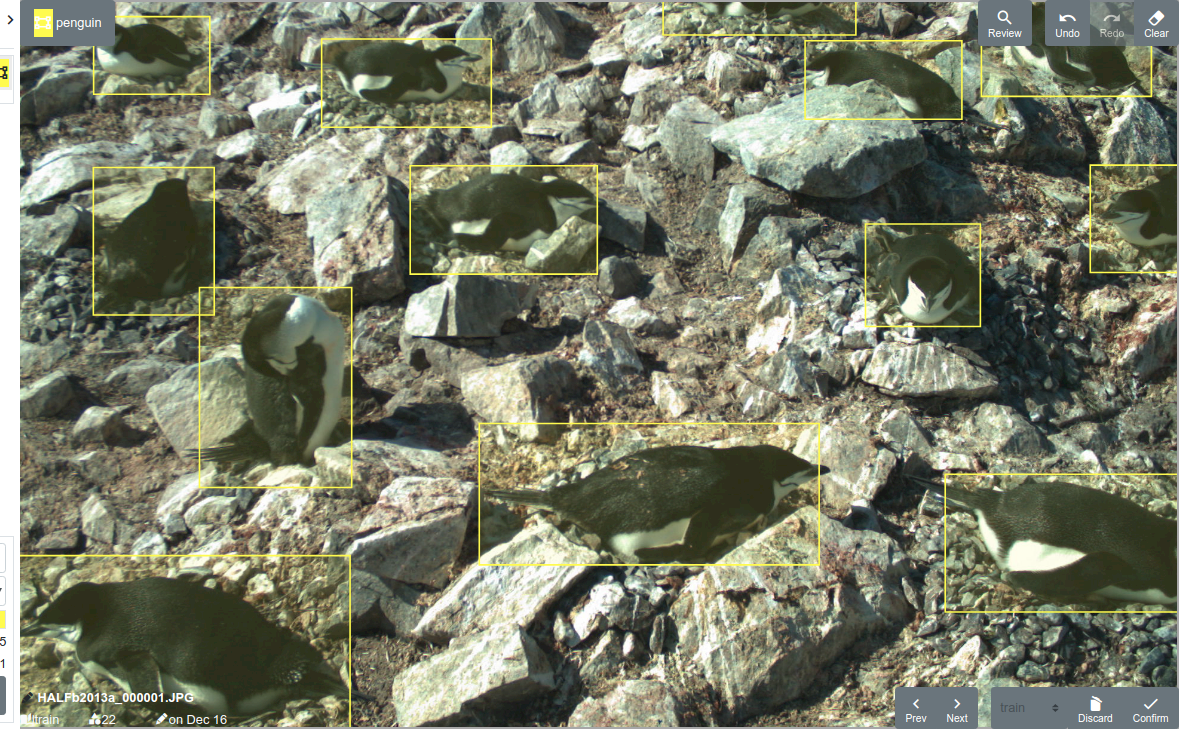
\includegraphics[width=1.0\linewidth]{figures/annotation/screenshots/penguins2.png}
   \caption{\emph{penguins}}
\end{subfigure}%
\begin{subfigure}[t]{0.24\linewidth}
  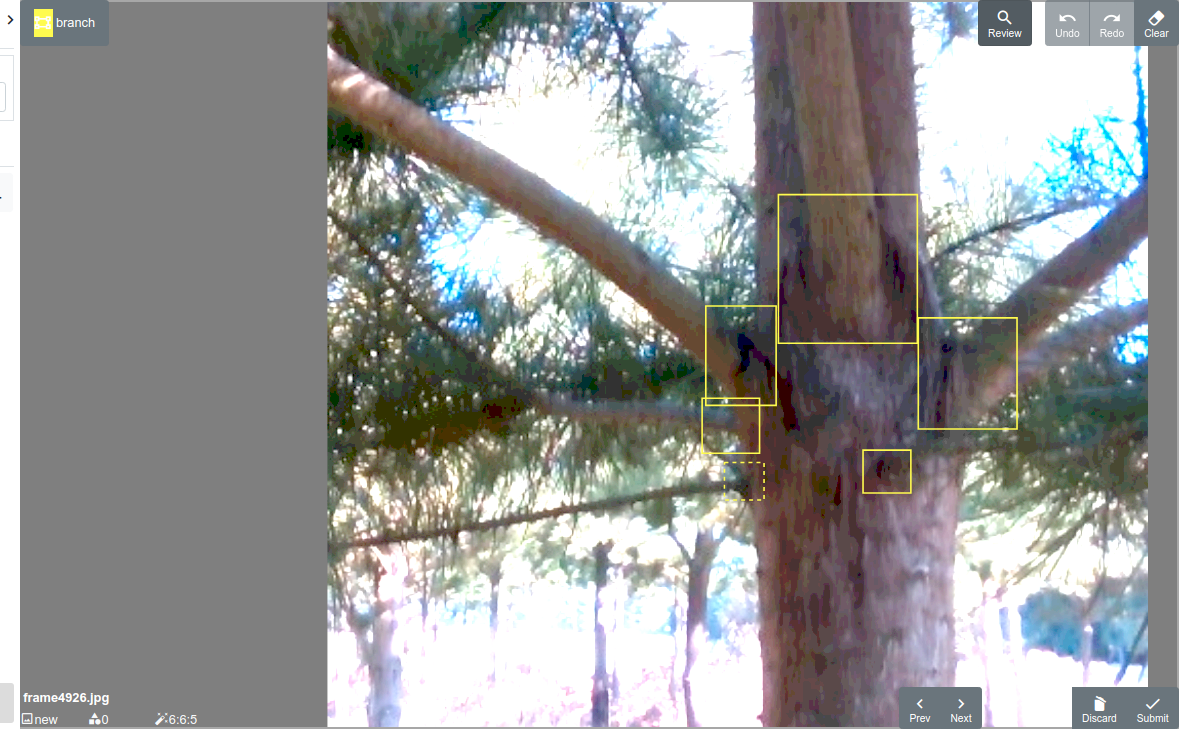
\includegraphics[width=1.0\linewidth]{figures/annotation/screenshots/branches3.png}
   \caption{\emph{branches}}
\end{subfigure}%
\begin{subfigure}[t]{0.24\linewidth}
  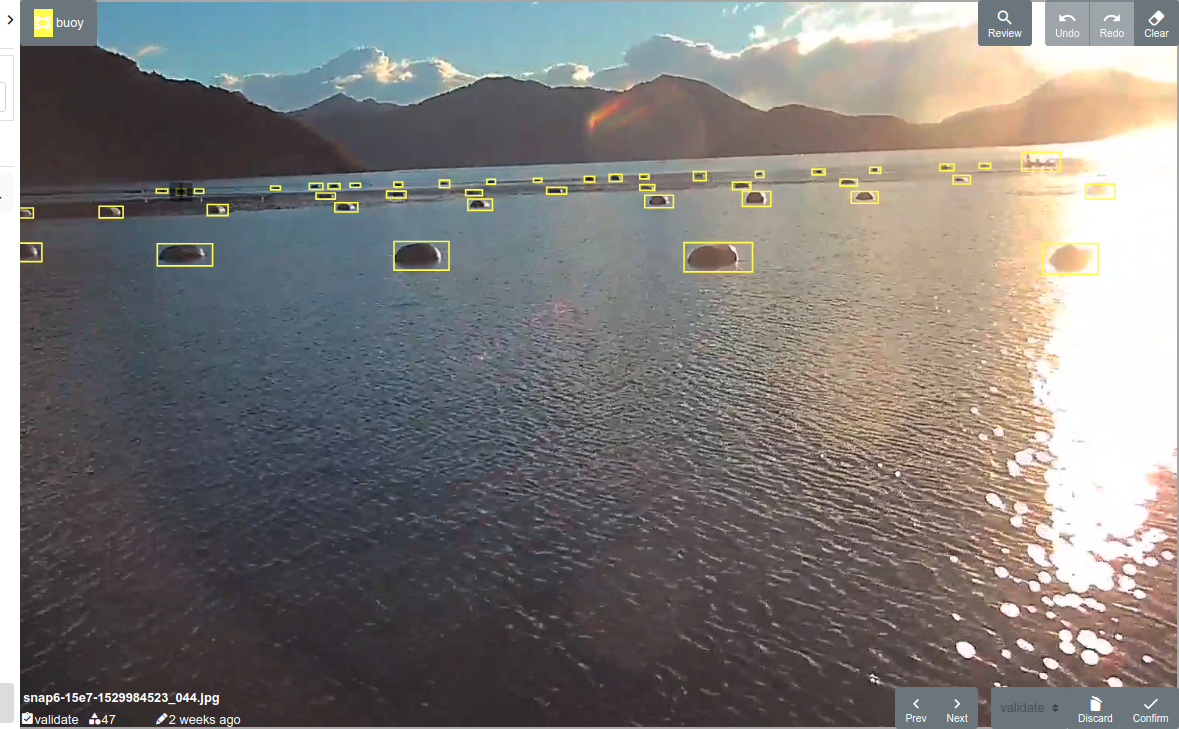
\includegraphics[width=1.0\linewidth]{figures/annotation/screenshots/buoys.png}
   \caption{\emph{buoys}}
 \end{subfigure}
\begin{subfigure}[t]{0.24\linewidth}
  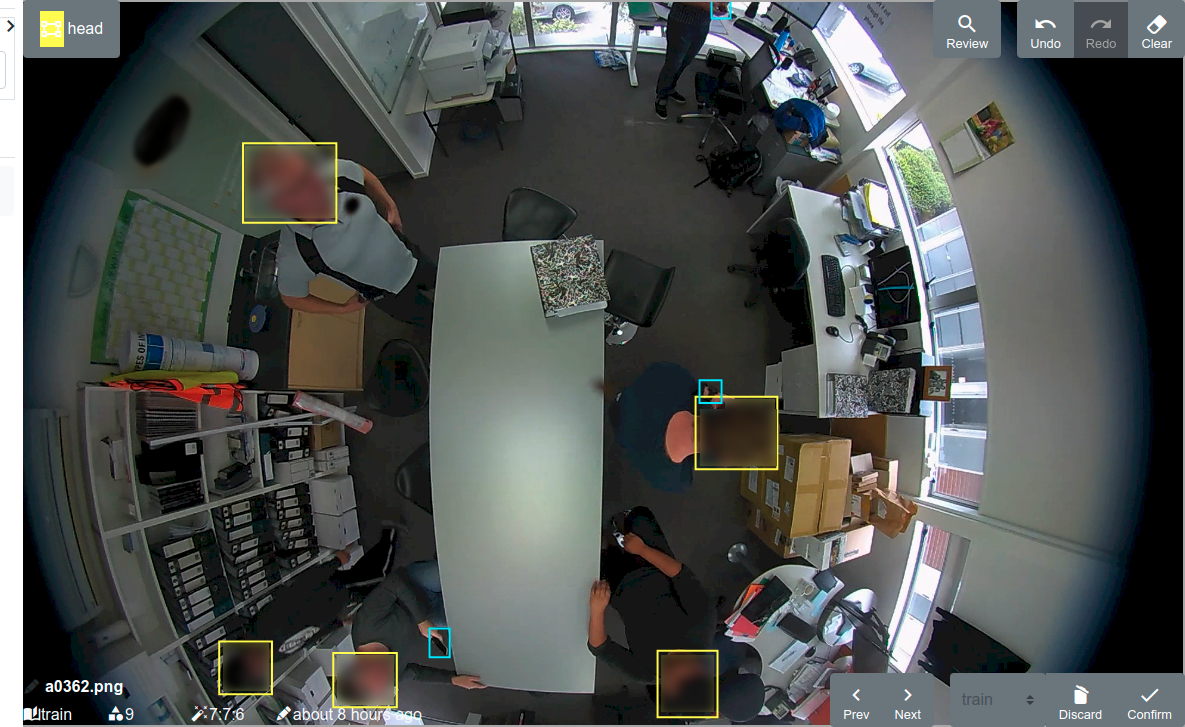
\includegraphics[width=1.0\linewidth]{figures/annotation/screenshots/victor.png}
  \caption{\emph{fisheye}}
\end{subfigure}%

\begin{subfigure}[t]{0.24\linewidth}
  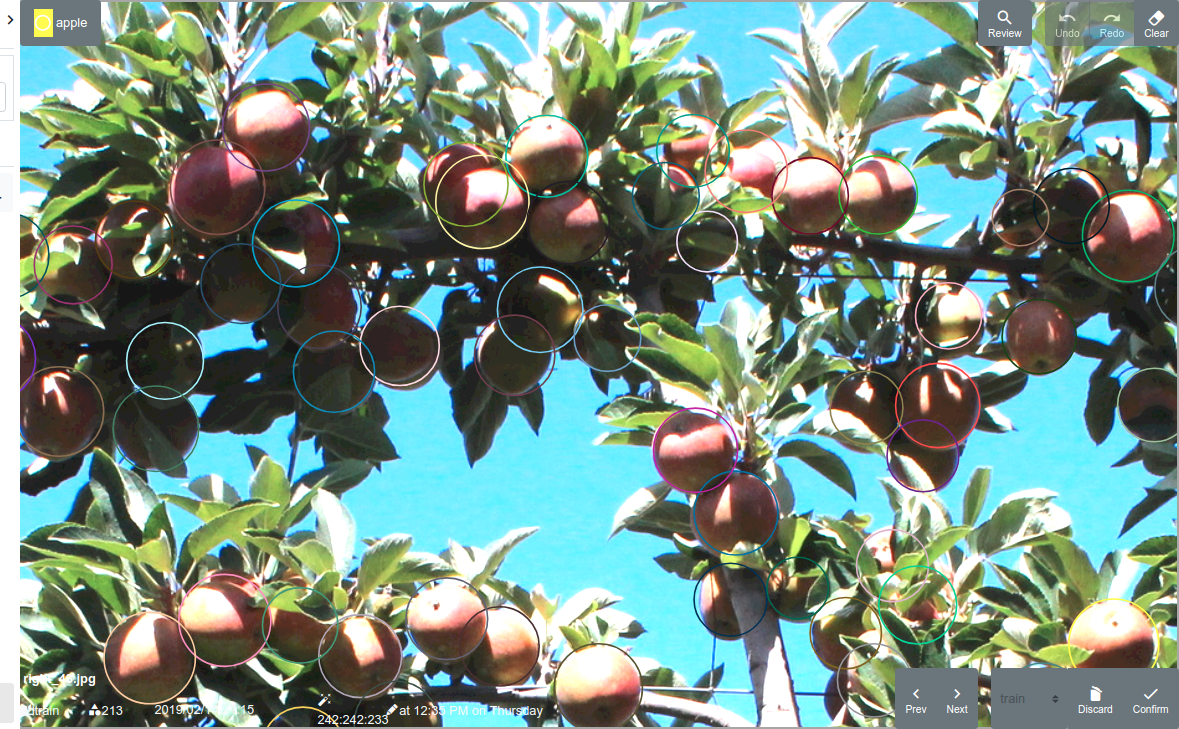
\includegraphics[width=1.0\linewidth]{figures/annotation/screenshots/apples_big2.png}
  \caption{$\mathrm{apples_1}$}
\end{subfigure}%
\begin{subfigure}[t]{0.24\linewidth}
  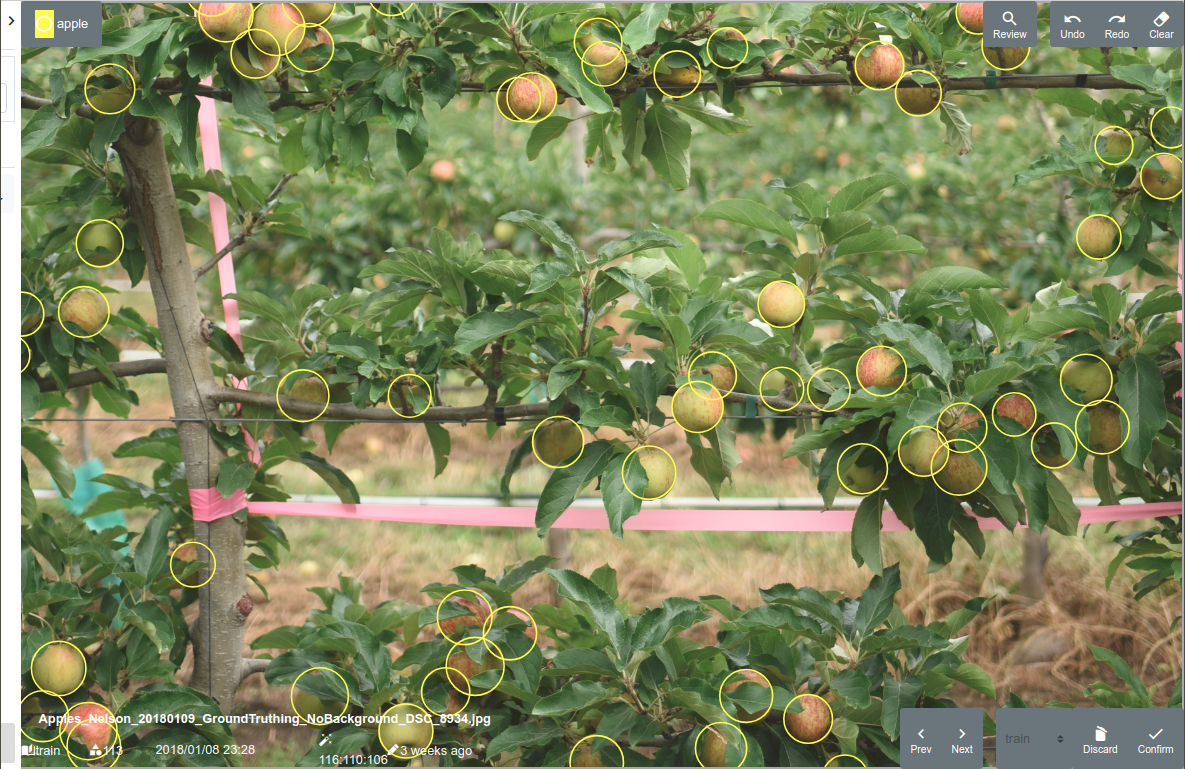
\includegraphics[width=1.0\linewidth]{figures/annotation/screenshots/apples2.png}
  \caption{$\mathrm{apples_2}$}
\end{subfigure}%
 \begin{subfigure}[t]{0.24\linewidth}
  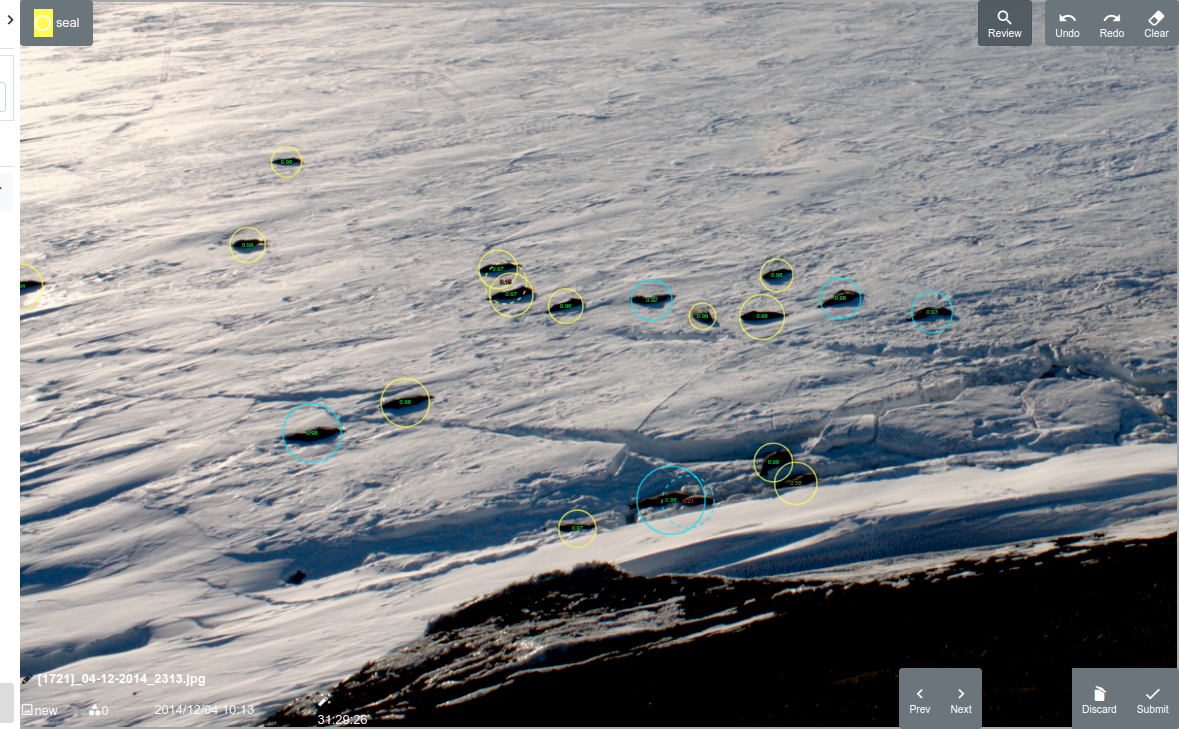
\includegraphics[width=1.0\linewidth]{figures/annotation/screenshots/seals_small2.png}
  \caption{\emph{seals}}
\end{subfigure}%
\begin{subfigure}[t]{0.24\linewidth}
  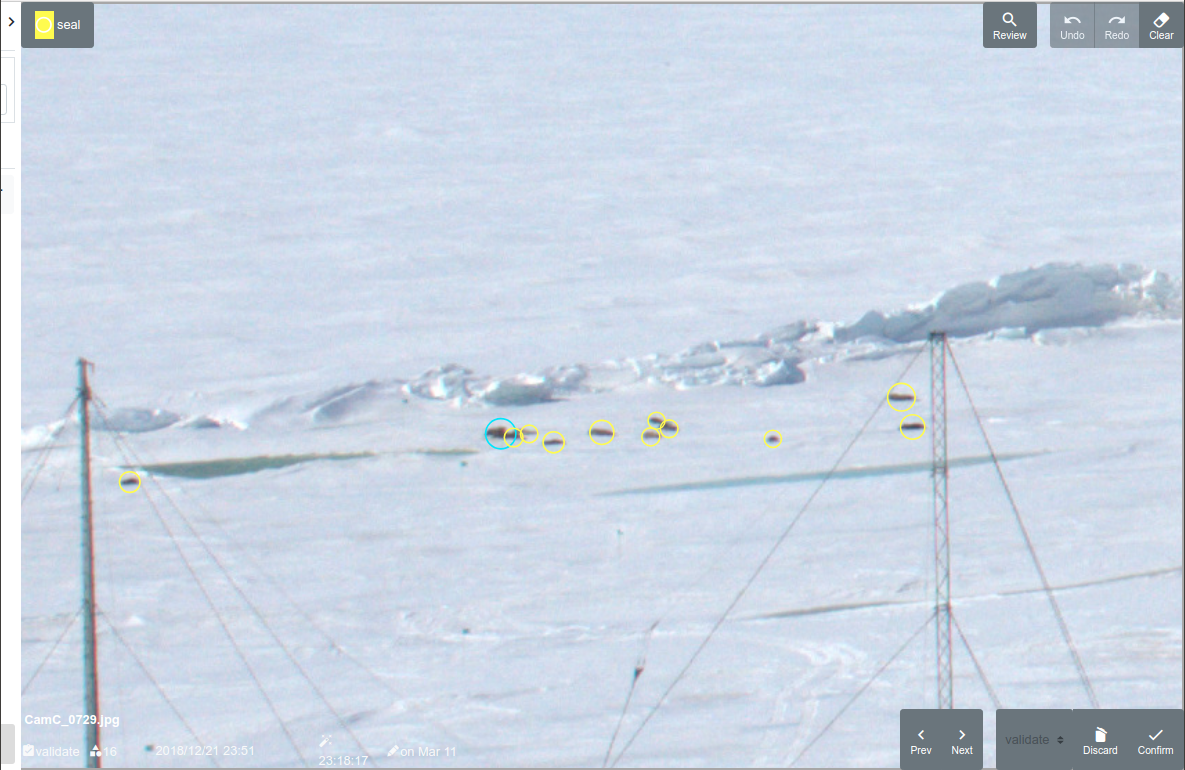
\includegraphics[width=1.0\linewidth]{figures/annotation/screenshots/scott_base_sunny.png}
  \caption{\emph{scott base}}
\end{subfigure}
\begin{subfigure}[t]{0.24\linewidth}
  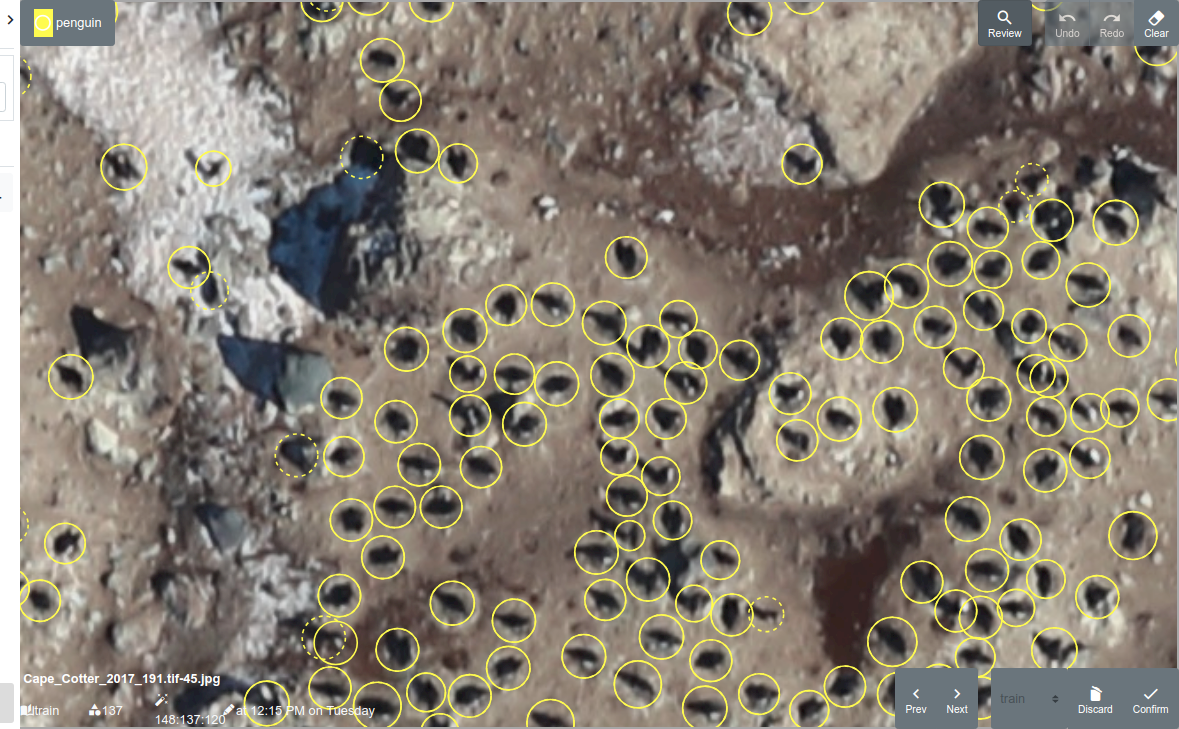
\includegraphics[width=1.0\linewidth]{figures/annotation/screenshots/penguins_aerial2.png}
  \caption{\emph{penguin survey}}
\end{subfigure}%
\begin{subfigure}[t]{0.24\linewidth}
  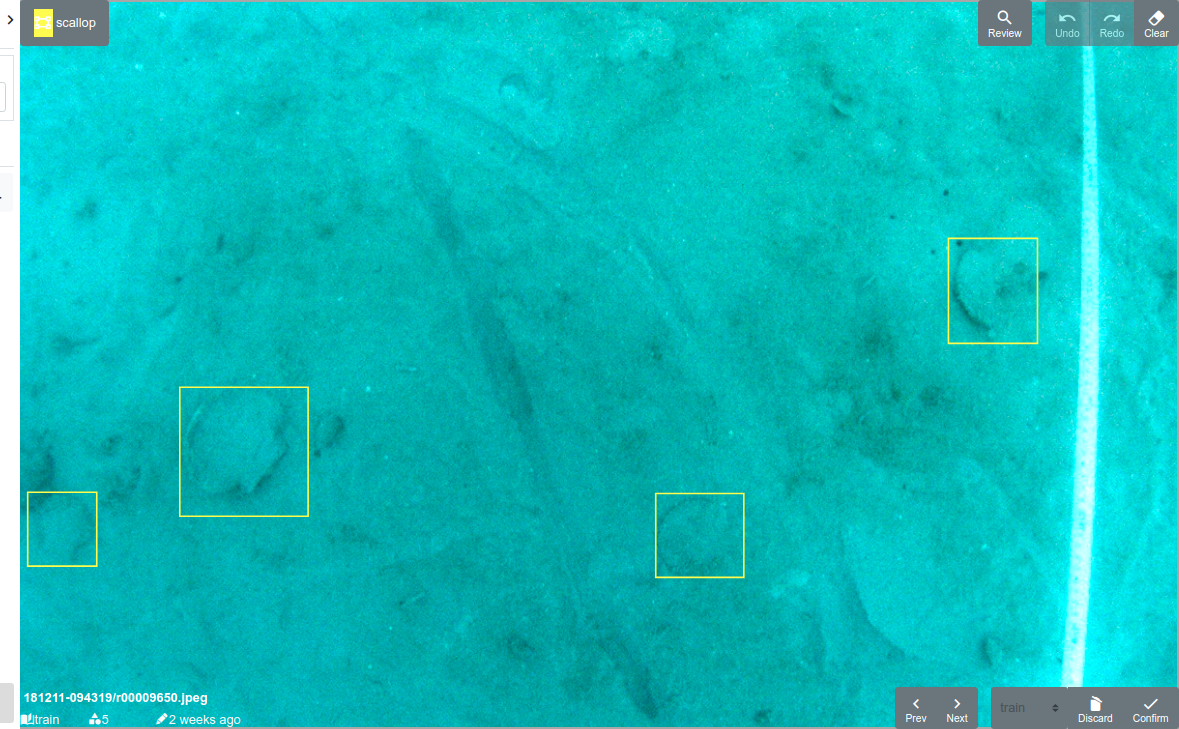
\includegraphics[width=1.0\linewidth]{figures/annotation/screenshots/scallops4.png}
  \caption{\emph{scallops}}
\end{subfigure}
\caption{Representative images of datasets (and annotations) annotated in this work}
\label{fig:datasets_all}
\end{figure}


In this chapter I present the results of an exploratory study, and demonstrate the practical use of the \gls{VBA} based annotation tool by annotating 10 image sets (several of them twice) on a variety of object detection tasks. Representative images are shown in figure~\ref{fig:datasets_all}. I analyse how the performance of the object detector changes as annotation progresses, with respect to the number and type of corrections required.

\section{Image sets and datasets}


The datasets comprise of firstly, a mix of relatively small scale image sets annotated for the sake of evaluating and developing the annotation method, and secondly, preliminary datasets as trial runs for larger scale annotation. A number also are annotated for a niche application, which seems suited to this kind of annotation method, in counting wildlife. Continuous annotation time (as defined below) was between approximately an hour for the smallest sets and up to eight hours for the largest.

\begin{threeparttable}[phtb]
\label{tab:resolutions}
\centering
\caption{Overview of datasets: number (n) and size of annotation, number and size of image.  } 
\begin{tabular}{lllllll}
dataset & n & images & box length & image size & \shortstack{training \\ crop} & \shortstack{validation \\ $AP_{COCO}$} \\
\toprule
$penguins$        & 7473        & 306    & $255 \pm 118$   &  $2048\times1536$  & 800                                   & 75.9                   \\
$branches$        & 2249        & 451    & $41.5 \pm 13.9$ &  $400\times400$    & 320                                   & 62.6                   \\
$seals$           & 4351        & 240    & $68.7 \pm 20.8$ &  $3920\times1600$  & 1024                                    & 80.7                   \\
$seals_b$         & 1256        & 82     & $63.4 \pm 17$   & $3920\times1600$  & 1024                                                     & 72.9        \\
$scott\:base$     & 7759        & 301    & $15 \pm 3.21$     & \shortstack[l]{$3927\times500$ -- \\ $5200\times700$} & 400  & 81.4  \\
$apples^1$        & 21637       & 300    & $78.4 \pm 14.9$ &  $2592\times1728$ & 1024 & 51.8                   \\
$apples^2$        & 13418       & 168    & $92.8 \pm 11.9$ &  $3008\times2008$  & 1024                                    & 74.5                   \\
$scallops_e$      & 3669        & 6741   & $114 \pm 40.2$  &  $1280\times1024$  & 800                                   & 65.0                   \\
$fisheye$         & 2598        & 367    & $96.6 \pm 32.7$ &  $2048\times1944$ & 1024                                     & 78.9                   \\
$buoys_d$         & 7221        & 207    & $38.9 \pm 42.8$ &  $1920\times1080$ & 600                                    & 70.9                   \\
\shortstack{$penguin$ \\ $survey$} & 13210       & 352    & $22.6 \pm 2.11$ & \shortstack[l] {$406\times405$ -- \\ $672\times448$} & 400  & 61.6               \\ 
\bottomrule
\end{tabular}
\begin{tablenotes}
\small
\item $*$ Subscripts denote different annotator, for example $seals_b$ is annotated by annotator $b$ where images from the same image set (not necessarily the same ones) are annotated by different users.  
\item $\ddagger$ Superscript denotes images from a different distribution of images
\item Datasets specified without subscript are annotated by the author.
\item $\dagger$ A bug relating to anchor box positioning impacted object detection. 
\end{tablenotes}
\end{threeparttable}


\subsection{penguins}
An image set used in the development of the annotation tool, primarily because the object detector performed well on the images after only a few annotated images and because of the relative uniformity of the images. The images used are a subset 'HALFb'  of the Penguin dataset \cite{PenguinData}, used for counting, using point annotations \cite{Arteta2016}. 
\subsection{$branches$}
An image set annotated as a test run for cut-point detection, where branch intersections (including hidden ones) are annotated with boxes by including the collar of the branch and a piece of the branch. Images are randomly sampled from a large set of frames extracted from several video sequences of orbits around trees. Images are lower resolution than other image sets ($ 320\times320 $ images), and a number of images have poor contrast.

\subsection{buoys}
An image set for monitoring mussel buoys. The ultimate idea is to monitor the growth of mussels by visually examining the height of the buoy out of the water, but this aspect is out of the scope of this work. Object detection is used as a first step however, and used to determine a water plane. Images are sampled from video sequences taken from a camera fixed to another mussel buoy. As a result the view angles are somewhat limited, but do change as the buoy (with the camera attached) rotates with the swell, with weather and lighting conditions also giving a variation to the appearance. 

Although image resolution is reasonably high ($1920\times1080$), there is a considerable number of visible artefacts from video compression. Buoys in the distance become very tiny, and were ignored once they became hard to distinguish. Buoys also tended to line up and occlude each other, so these buoys were also ignored.


\subsection{fisheye}
    
A test for detecting people (heads) and cellphones in roof mounted fisheye camera images. Trained models for human detection (and pose recognition) are readily available but fail on fisheye images because the orientation and scale of an object changes, dependent on their position in the image. Person detection worked almost immediately after a handful of images, with only minor corrections required, however, cellphone detection required more intervention, but began to work reliably towards the end of annotation. Experiments afterwards showed that the high-resolution ($2048\times1944$) was necessary to detect the cellphones; detection failed at half resolution.

\subsection{$\mathrm{apples^1}$}

A set of images of trellised apple trees with many apples per image. Only the apples in the foreground were annotated; small apples and cherries in the background provided distraction. Leaves occlude a large number of apples in the image set, however, all apples which could be located were annotated. Often, it is possible to guess quite accurately the location of the apple because a section of the curved outline can be seen, although it is harder to accurately guess the size of the apple. 

Images were taken with a high-resolution DSLR camera and scaled to half resolution ($2592\times1728$); apples in the photos at this resolution are large ($50$-- $200$ pixels, median $80$). Despite only annotating 300 images, this dataset has the most annotations (over $22000$) and took longest to annotate. Lighting was often less than ideal as direct sunlight caused poor contrast in many images.
    
\subsection{$\mathrm{apples^2}$}
    
Another set of images of trellised apple trees; when compared to \emph{$apples^1$}, has a higher degree of  photographic consistency (resulting in more consistent sizes and number of apples), and better focus on the foreground (less distracting background with some images, additionally, given a black backdrop). These differences manifested themselves in the difference in validation accuracy seen in table~\ref{tab:validation_corrections}, reaching a higher accuracy than \emph{$apples^1$}.

While at a similar resolution to \emph{$apples^1$}, some images were captured as portrait as well as landscape orientation, whereas all the images in \emph{$apples^1$} are landscape orientation. The same annotation strategy was used between both sets, to annotate all apples which can be localised.

\subsection{seals}
    
 A time series sequence of images taken as part of the \emph{Turtle Rock Seal Survey} \cite{Eisert2015}. The images are captured 10 minutes apart, taken of part of an Antarctic Weddell seal colony around Turtle Rock, an island approximately 12km north of Scott Base. The time period was a three week period from the 28th November to the 19th of December, 2014. The purpose of this monitoring is to establish haul-out patterns where seals sit on the ice (in order to avoid predation).  

Images were taken from a high-resolution DSLR camera and cropped to give a resolution of $3920\times1600$. The images were annotated twice. Different images were annotated in both cases, a result of random selection. Separate test sets, using the same images in both cases, were created before annotation began. From a set of $3000$ images, the first $240$ images were annotated by the author and the second $82$ by user $b$. The test set comprised $46$ images.

The seals generally sat well separated from each other and were very clearly distinct, except for mother and pup combinations who often sat right next to each other. Lighting was occasionally quite difficult for observations. Seals were annotated as two classes, either: (a) single seal or (b) mother next to pup.  The misclassification of mother and pup vs. single seal was the largest source of error during annotation and in validation. Disambiguation of the two is difficult for a human without viewing the images in the time series, where it becomes apparent due to the seal's movement.

More details can be found in section~\ref{sec:case_seals}.

\subsection{scott base}
    
Another time series sequence of images, part of the \emph{Weddell Seal Abundance Monitoring Programme} \cite{Eisert2019}. Images were captured 10 minutes apart, taken of Weddell seals around Scott Base, Antarctica. Two different views were used in this work (three views were captured, but the third view was not used as it contained few seals in the time period used here). The purpose is for population monitoring annually to be able to evaluate the impact on the seal population when Scott Base is renovated in the coming years. 

Two different DSLR cameras were used, each with a different viewpoint (and different image size). Images were cropped to the regions containing seals, as they were very wide, and $5000\times700$ from one viewpoint. The viewpoints, unlike the \emph{seals} images, were from far away and the seals were tiny (a mean of $15$ pixels diameter) with considerable blurriness.  
    
More details can be found in section~\ref{sec:case_seals}.
    
\subsection{penguin survey}
    
The images are from the Ad\'elie Penguin Census \cite{Lyver2014}, an aerial photographic survey (started in 1981 and continuing until the present) in which a complete census of the Ad\'elie penguin population is taken by counting nesting pairs. High-resolution photographs are taken from an altitude of 2000-2500 feet.

Three separate annotations are performed; two of them from images comprising part of two large colonies, and one from a distinct and much smaller colony in 3 separate images. In each case, the large images are broken into small images for practical reasons, including the number of annotations the software can handle, as well as the number of annotations which are  practical for an annotator to check in one go.
    
The images, once chopped into pieces, are relatively small, but still contain large numbers of penguins, comparable to $apples^2$ in terms of annotation per image (see figure~\ref{fig:instances_image_plot}). The penguins themselves are small and blurry, with two forms, either sitting or standing. These become  easily confused, and also difficult to distinguish from the shadows in rocky areas and are considerably ambiguous. 

\subsection{scallops}
    
These images are drawn from video frames taken by an underwater \gls{ROV} used to survey a small seabed area containing scallops. The images are unique from the others used in this work, in that the object instances are very sparse; there are many images with no scallops. 

The images are part of a project intending to survey scallops, and eventually develop methods of mechanically harvesting them. The usual current method of harvesting scallops is by dredging the sea floor, an environmentally destructive method. By harvesting scallops individually, the destruction of the sea floor can be avoided.

These images are an initial test run of both image capturing and annotation. The lighting on the \gls{ROV} went out mid capture, leading to approximately half the images appearing in good lighting and the other half in dim blue natural light. The point of view also changed mid capture, some images being forward facing, and others downward facing. The images often traversed backwards and forwards across the same areas, thus limiting the visual appearance (often seeing the same scallop repeatedly). 

The annotation of the scallops dataset was performed by a combination of two scallop experts. It was intended as a trial of example selection, and was initially configured to select images in order of highest detection count (done by the first annotator). However, after approximately $120$ minutes ($25\%$ of the time), a second annotator took over and annotated the rest of the frames in sequence. 

The annotation criteria was that to be annotated, the scallop must be clearly visually alive; due to the turbidity of the sea water this meant that scallops are more uncertain further from the camera. Due to the criteria for annotation, this meant that often the same scallop was marked as positive in one frame and negative in the next. 

Training the object detector on the scallop dataset was more unstable in validation accuracy than other datasets annotated here (see figure~\ref{fig:datasets_lr} and figure~\ref{fig:scatter_loss_ap}). Given the differences between visual appearance in the source images (for example those with artificial light and those with natural light), combined with the discontinuous annotation criteria, it seems this is likely to blame for the apparent instability seen in training. 

In future, the plan for a larger scale annotation involves annotating scallops with a range of uncertainty, where the criteria is not \emph{scallop} or \emph{not scallop}, but \emph{scallop} with a degree of uncertainty, and only \emph{not scallop} when the object in question is definitely not a scallop. The sparseness of the scallop instances makes image selection relatively much more important; this is apparent when examining user actions in figure~\ref{fig:actions_dataset_b}, where it can be seen that the most common action by far is to \emph{submit} an image.



\begin{table}[]
\centering
\caption{ Statistics of user actions over annotations (anns.) of different datasets }
\label{tab:annotation_table}
\begin{tabular}{llllll}
dataset           & actions & anns. & \shortstack {ann. time \\ (minutes)} & \shortstack{instances \\ per minute} & \shortstack{actions \\ per ann.} \\
\toprule
$penguins$        & 2,070   & 7473        & 140                       & 53.5                 & 0.28                   \\
$branches$        & 745     & 2249        & 63                        & 35.7                 & 0.33                   \\
$seals$           & 587     & 4351        & 89.8                      & 48.5                 & 0.13                   \\
$seals_b$         & 453     & 1256        & 76.4                      & 16.4                 & 0.36                   \\
$scott\:base$     & 1,499   & 7759        & 123                       & 63.1                 & 0.19                   \\
$apples^1$        & 5,542   & 21637       & 511                       & 42.4                 & 0.26                   \\
$apples^2$        & 3,710   & 13418       & 364                       & 36.9                 & 0.28                   \\
$scallops_e$      & 2,065   & 3669        & 561                       & 6.54                 & 0.56                   \\
$fisheye$         & 337     & 2598        & 58.4                      & 44.5                 & 0.13                   \\
$buoys_d$         & 1,230   & 7221        & 234                       & 30.9                 & 0.17                   \\
$penguin\:survey$ & 1,616   & 13210       & 120                       & 110                  & 0.12                  \\
\bottomrule
\end{tabular}
\end{table}



\section {Evaluation methods}
\label{sec:ann_evaluation}

The primary method of evaluation used in this work is that of \emph{continuous testing}, whereby it is possible to characterise how the annotation process changes over time; how the model's predictions impact on the actions taken by the annotator, the type of actions and time required, and the accuracy of the model's predictions.

User edits are logged, along with predictions provided by the model (the starting point for annotating each image), and the final set of annotations submitted by the user. The accuracy of detections are verified directly by the user, giving continuous testing of the model predictions on unseen images as they're annotated.

The types of actions as well as the timing can provide useful cues as to the difficulty of the task, and the level of assistance provided by the object detection model. I break down these actions, and the relation of the actions to the original set of detections to the performance of the object detector in a few different ways: categorise the action types and frequencies; categorise the corrections applied to each annotation; and lastly use a locally weighted \gls{AP} to quantify object detection performance on newly annotated images.

\subsection{User actions}

The various user actions are discussed in section~\ref{sec:user_interface} in more detail. For the purposes of this chapter the user actions are broken down into categories:

\begin{itemize}
    \item {\bf transform}: an annotation is transformed (scaling, translation, corner dragged).
    \item {\bf confirm}: a weak detection is confirmed. This may also include a transformation of bounding box, but it is performed as one action.
    \item {\bf delete}: one or more annotations are deleted.
    \item {\bf add}: a new annotation is added.
    \item {\bf set class}: the class of an annotation is changed.    
    \item {\bf submit}: an image is submitted.    
\end{itemize}

\subsection{Annotation corrections}
\label{sec:corrections}

Another way of analysing the annotation process is to categorise each annotation by the nature of corrections applied to the original machine prediction (or lack of). This differs from user actions because: (a) multiple actions may be performed on one annotation, for example, a scaling and a translation, or changing the class and translation and (b) one action may modify multiple annotations, frequently a deletion of multiple false positives at once.

The following definitions are used:

\begin{itemize}
    \item {\bf positive}: a high confidence detection unchanged after verification.
    \item {\bf modified}: high confidence detection where either the box annotation or the class label has been modified.
    \item {\bf weak positive}: a weakly confident detection confirmed using the review mode (and potentially transformed).    
    \item {\bf false negative}: an object which was missed by the object detector and annotated manually by the user.    
    \item {\bf false positive}: an incorrect high confidence detection deleted by the user.
\end{itemize}

\subsection{Measuring progress with Cumulative Annotation Time}
\label{sec:ann_time}

\begin{figure}[ht!] 
\centering
  \includegraphics[width=1.0\linewidth]{charts/summaries/time_density.pdf}
  \caption{Time per action distributions for different dataset annotations}
  \label{fig:annotation_time_density}
\end{figure}

There are several ways progress could be measured in terms of annotation progress, such as the time spent since annotation began, the number of images or annotations submitted or \gls{CAT}, which we use in analysis for this chapter, which is the total time the user has spent actively using the tool.
 
In section~\ref{sec:schedule}, experiments in incrementally training on a dataset validation accuracy to be strongly dependent on the number of examples used. Annotation in general takes longer than training, and extra training without extra annotation generally has no positive effect.

For the above reason I use annotation time as opposed to training time, to measure and visualise the annotation progress. These assumptions  may change depending on the difficulty of the problem, complexity of a model or with many annotators contributing.



\subsection {Breaks in annotation}
\label{sec:break_detection}

The annotation logs recorded in this chapter were not taken in a controlled experimental setting, although an effort was made to be consistent in datasets annotated by the author. Datasets annotated by others can be seen to have more variability. It was therefore necessary to detect breaks where annotation was paused mid-image. Any action was capped at a maximum of one minute for this purpose. Ideally this would have been detected directly in the tool by detecting lack of input or loss of focus, and future studies will take this approach. 

Figure~\ref{fig:annotation_time_density} shows the distribution of times per action for different annotation efforts where any action taking more than a minute is a significant outlier in most cases. An obvious discrepancy can be seen between the \emph{scott base}, \emph{seals} and \emph{scallops} datasets, this is because the video sequences are useful in resolving ambiguity and more time is spent looking forward and backward at previous frames.

\subsection{Visualisation}
\label{sec:visualisation}

In order to visualise trends in the user action types, a fixed size density estimation is used with a gaussian kernel, $\sigma=5 minutes$. This approach is taken for both user actions, annotation correction types, the rate of annotations and using a weighted \gls{AP} to quantify overall detector performance at a particular point in  time.

Annotation actions, and corrected annotation types are all deemed to occur at the \gls{CAT} the image is submitted. Even though actions occurred at distinct points during an image annotation, the interest is in overall trends rather than particular trends within annotating each image. 

\subsection {Locally weighted Average Precision}
\label{sec:noisy_trends}

To give a single metric for object detection performance, where parts of a dataset are more important than others, I use a weighted \gls{AP}. The object detector's predictions are compared against the user's final annotations. A standard matching procedure is performed for all images (as opposed to tracking the user edits as in section~\ref{sec:corrections}).

In order to align with user actions across \gls{CAT}, a locally weighted \gls{AP} is used. To evaluate the locally weighted \gls{AP} at a particular point in cumulative annotation time, each image is given a weight according to its time difference from the image \gls{CAT}. As above, the gaussian kernel with $\sigma=5 minutes$ is used.

Annotations in each image are weighted by the image weight for the purposes of counting false positive, false negative and true positive counts. From there, weighted precision and recall and \gls{AP} are computed exactly as normal (see section~\ref{sec:evaluation_metrics}).


\section {Dataset overview}
\subsection {Size distribution}

\begin{figure}[ht]
\centering
\includegraphics[width=1.0\linewidth]{charts/summaries/sizes_density.pdf}
\caption{Object bounding box size distributions as percentage of the object size to the image size (average of width and height) }
\label{fig:box_sizes}
\end{figure}
 

\begin{figure}[ht]
\centering
\includegraphics[width=1.0\linewidth]{charts/summaries/sizes_boxplot.pdf}
\caption{ Distribution of object box sizes in pixels for all datasets. Box plot showing quartiles, range and median (red line) on a log scale. Size here is measured as the larger side length in pixels. }
\label{fig:box_sizes_plot}
\end{figure}

The sizes of objects in these datasets, in general, are small compared to more mainstream object detection datasets. This can be seen in figure~\ref{fig:box_sizes}, where compared to the Pascal VOC \cite{Everingham2008}, or COCO \cite{Lin2014}, the box sizes are smaller compared to the image size and less widely distributed. 

Figure~\ref{fig:box_sizes_plot}  shows the distribution of object sizes (in pixels) of all the datasets together for comparison. In particular, the \emph{penguin survey} and \emph{scott base} datasets have particularly tiny objects.

It can be seen that although the box sizes are relatively small, compared to the image, that for high-resolution images the objects can still be relatively large in pixels.

Two different types of annotations are used in the annotations of these datasets. Circular annotations are used for very small objects and for counting objects where precise localisation is of less concern; circular annotations are also used for apples, where it just happens to match the object shape well. The difference to the object detector is that a centre and radius is estimated (instead of centre, width and height). The circles are treated as a square for computations such as \gls{IOU} overlap.

\subsection {Instance distribution}

\begin{figure}[ht!]
\centering
\includegraphics[width=1.0\linewidth]{charts/summaries/instances_boxplot.pdf}
\caption{ Distribution of object annotations per image, shown as a box plot with quartiles, range and median (red line) on a log scale. Vertical coloured lines show annotation counts for particular images. }
\label{fig:instances_image_plot}
\end{figure}

\begin{figure}[ht]
\centering
\includegraphics[width=1.0\linewidth]{charts/summaries/duration_boxplot.pdf}
\caption{ Per image annotation time distributions as box plot showing range, quartiles and median (red line). Vertical lines are individual images with line length proportional to to $\sqrt{|annotations|}$. }
\label{fig:duration_boxplot}
\end{figure}

The datasets in question have a wide range of instance distributions, shown in figure~\ref{fig:instances_image_plot}. Some such as \emph{apples2}, \emph{branches}, \emph{fisheye} and \emph{penguins} contain relatively uniform numbers of annotations. Others, especially \emph {penguin surveys}, \emph{scott base} and \emph{apples1}, contain a wide range (a few with several hundred annotations per image). One dataset, \emph{scallops}, contains very few annotations ($0.54$ per image), where most images are negative images.

\subsection {Impact of instance count on verification}
\label{sec:impact_instances}

The instance distribution in each image has clear implications for verification based image annotation. Verifying several instances at once can be more efficient than one at a time, but verifying too many instances concurrently increases cognitive load (the very problem human-in-the-loop machine learning seeks to address). 

Despite the ability to zoom into a small part of an image, in order to submit an image, the user must review the whole image or remember which parts have been checked. For this reason, when images become excessively large, they should be split into pieces which can be easily verified without too much use of navigation.

This can be similar to a user interface for navigating search results, where showing several results at once is much faster for a user to peruse, than showing them one by one. However, if too many results are shown on each page, the results become lost in the crowd. A pair of studies found users do not look at results beyond 30 per page \cite{PunchoojitLumpapun2017, Zhou2007}.

The dual threshold approach helped in this regard, by highlighting areas of uncertainty. For some datasets, \emph{penguin surveys}, \emph{apples1} and \emph{apples2}, the number of instances made it hard to keep track of progress when verifying the whole image. Combined with uncertain instances, which are difficult to see without zooming, checking to ensure all annotations are present becomes difficult.

The dataset \emph{scott base} also suffers a little from this problem. The images are much wider than they are long, making navigation somewhat tedious, and verifying the whole image much harder by having to zoom right out to check the whole image. In future some method of marking parts of an image, as checked, may be useful.

\section {Annotation overview}
\label{sec:annotation_overview}

Here,  I try to break down any major trends seen from both annotation logs and the set of initial detections and final annotations. To begin with, I summarise the user actions and how they relate to the types of corrected detection. I also look at the object detection performance in validation, compared to the rate of true and weak positives for each dataset.

\subsection {Actions and corrections}

\begin{figure}[ht!] 
\centering
\begin{subfigure}{0.48\linewidth}
\includegraphics[width=1.0\linewidth]{charts/summaries/correction_counts.pdf}
\caption{}
\label{fig:actions_dataset_a}
\end{subfigure}%
\begin{subfigure}{0.48\linewidth}
\includegraphics[width=1.0\linewidth]{charts/summaries/action_counts.pdf}
\caption{}
\label{fig:actions_dataset_b}
\end{subfigure}

\caption {(a) Total corrected detection types as a proportion of total annotation count. Note, totals do not sum to $1.0$ for two reasons: firstly false positives are shown, secondly positive detections are not. (b) Proportions of total actions. }
\label{fig:actions_dataset}
\end{figure}

\begin{table}[h!]
\caption{Validation accuracy at relaxed and strict IoU thresholds compared with proportions of corrected detections for each dataset}
\label{tab:validation_corrections}
\begin{adjustbox}{max width=\textwidth}
\begin{tabular}{llllllll}
dataset           & \shortstack{validation \\ $AP_{50}$} & \shortstack{validation  \\ $AP_{75}$} & positive & \shortstack{modified\\ positive} & \shortstack{weak\\ positive} & \shortstack{false \\ negative} & \shortstack{false \\ positive} \\
\toprule
$penguins$        & 99.4      & 90.5      & 82.6\%   & 12.3\%            & 2.9\%         & 2.3\%          & 0.8\%          \\
$branches$        & 95.7      & 69.6      & 76.8\%   & 6.4\%             & 10.2\%        & 6.3\%          & 2.7\%          \\
$seals$           & 95.5      & 93.1      & 93.4\%   & 4.1\%             & 1.9\%         & 0.6\%          & 1.8\%          \\
$seals_b$         & 92.0      & 81.5      & 87.3\%   & 1.1\%             & 0.0\%         & 11.7\%         & 8.7\%          \\
$scott\:base$     & 97.5      & 92.7      & 84.8\%   & 1.0\%             & 11.4\%        & 2.8\%          & 0.7\%          \\
$apples^1$        & 67.6      & 59.9      & 75.1\%   & 5.1\%             & 11.2\%        & 6.1\%          & 3.5\%          \\
$apples^2$        & 94.5      & 83.7      & 76.1\%   & 9.8\%             & 8.5\%         & 5.3\%          & 1.2\%          \\
$scallops_e$      & 92.8      & 78.4      & 62.3\%   & 4.9\%             & 2.1\%         & 30.4\%         & 9.5\%          \\
$fisheye$         & 99.3      & 90.7      & 91.8\%   & 2.4\%             & 4.1\%         & 1.5\%          & 0.4\%          \\
$buoys_d$         & 96.8      & 83.2      & 89.9\%   & 2.0\%             & 3.9\%         & 4.1\%          & 3.5\%          \\
\shortstack {$penguin$ \\ $survey$} & 90.9      & 73.3      & 89.5\%   & 0.5\%             & 7.5\%         & 2.4\%          & 1.1\%        \\ 
\bottomrule
\end{tabular}
\end{adjustbox}
\end{table}

The type of user actions performed, and the type of corrected detection can be seen in figure~\ref{fig:actions_dataset} and in more detail in table~\ref{tab:validation_corrections}. The two actions and correction types are different because: (a) multiple actions may be needed to correct one detection, and (b) one action can modify multiple detections, for example, deleting a group of false postives (this can be seen in the discrepancy in $apples^1$ where groups of false positives occur, to begin with, in images showing people, cars and wider angle shots). 

The action \emph{transform} is the most common action, by a long way, in the three datasets, and is significant in all other datasets (except \emph{scallop}, only because \emph{submit} outweighs the rest by such a large amount). This idea is not quite so well shown in the breakdown by corrected detection type, where \emph{modified positive} does not feature as prominently, mainly because the \emph{weak positive} category also includes low confidence detections which were transformed. This is not reflected in figure~\ref{fig:actions_dataset_b} because the user action \emph{confirm} is conflated with \emph{transform}. In cases where a user transforms a weak detection, it is confirmed at the same time yet counted as \emph{transform} only.

The most common action in three (and almost four) datasets is \emph{submit}, but this occurs for different reasons. In the \emph{scallop} images, it occurs because of the sparsity of object instances. In the \emph{fisheye} images, which have a very uniform visual appearance, the object detector reaches near human-level detection performance and there is nothing for the annotator to do except submit the provided detections.

One outlier which can be seen is $apples^1$, where the validation scores are much lower than $apples^2$, yet the correction statistics are very similar, with a similar positive proportion, albeit with $apples^1$ having higher proportions of false positive and false negative. It is not apparent exactly why this is the case, one possibility is that the validation set split is simply full of harder examples, and hence further investigation is necessary.

\subsection{Annotation rate}
\label{sec:annotation_rate}

\begin{figure}[ht!]
\centering
\includegraphics[width=1.0\linewidth]{charts/summaries/cumulative_instances_crop.pdf}
\caption{ Cumulative instances annotated (truncated to first 140 minutes)  }
\label{fig:cumulative_instances}
\end{figure}

\begin{figure}[ht!]
\centering
\includegraphics[width=1.0\linewidth]{charts/summaries/instance_rates.pdf}
\caption{ Annotation rate for all datasets (instances per minute) across annotation period, density plot with $\sigma=5minutes$ }
\label{fig:annotation_rate}
\end{figure}


\begin{figure}[ht!]
\centering
\includegraphics[width=1.0\linewidth]{charts/running_maps/overall.pdf}
\caption{ Locally weighted $AP_{COCO}$ of detections with respect to corrected annotations, providing a single metric taking into account all user corrections }
\label{fig:average_precision_test}
\end{figure}

The annotation progress can be most simply seen by examining firstly, the cumulative instances annotated in the given annotation time, and secondly, the rate of annotation occurring. Figure~\ref{fig:cumulative_instances} shows the cumulative instances over a $150$ minute period from the start of annotation. Figure~\ref{fig:annotation_rate} shows the rate of annotation (using a density plot of annotations added with a gaussian kernel of $\sigma = 5 minutes$). In this case the full annotation period is shown, where time is expressed as a percentage of total annotation time, instead of minutes.

A general acceleration in annotation can be seen in the  cumulative instances and more clearly seen in the annotation rate, although progress is far from linear. Time and instances are clearly not the only factors influencing annotation rate. 

The datasets with the most uniformity can be seen to provide the most benefit. They are the time series datasets, especially from video, where \emph{fisheye}, \emph{penguins}, \emph{seals}, and \emph{scott base} show the most clear benefit. These same datasets can be seen to be the ones which provide the most accurate detections, and also are the ones which achieve the highest validation accuracy (see table~\ref{tab:validation_corrections}).

Notably, missing from these figures is the \emph{penguin survey} dataset, as it is actually a combination of three annotation runs on separate parts of the \emph{penguin survey} dataset from different geographical locations. Discussion around this is given in section~\ref{sec:case_penguins}.

The scallop dataset is a particular outlier, the image selection policy changed from selection by maximum detection to sequential frame-by-frame at the first $25\%$ or $120 minutes$. Due to the sparseness of positive examples at various parts of the video sequences. The object detection accuracy can be seen to degrade at that same point figure~\ref{fig:average_precision_test}, possibly because of the influx of negative examples or a domain shift (the images varied in view angle between runs, and the light on the \gls{ROV} became intermittent). Towards the end of annotation, the object detection performance recovers, along with the annotation rate. Given this result, it would seem prudent to focus image selection policy on obtaining a balanced training set. 

\section{Discussion}
\label{sec:discussion}

\subsection{Verification threshold}
\label{sec:verification_threshold}

Behind any tool based on verification (be it cross verifying human annotation, or verifying machine predictions), there are implicit thresholds which are deemed acceptable and are going to vary between person to person and even within one person's verification effort. 

How often an object detector can exceed the annotator's verification threshold, will largely determine the level of assistance provided by a verification based tool (along with other factors like false positives and accurate classification). For the datasets annotated here, this can be seen in table~\ref{tab:validation_corrections}, where there is a range between $60\%$ and $90\%$ of verified detections accepted as is (across the whole annotation effort). 

\subsection{Algorithmic limits}
\label{sec:machine_limits}

The benefits of a \gls{VBA} tool are limited by the object detector. The benefit provided can (and does) increase as more images are annotated and the object detector becomes more accurate, but is also bound by the algorithms used by the object detector. Some datasets annotated here, were negatively impacted by the inability of an anchor-box based object detector to detect overlapping objects, particularly in the two apple datasets and \emph{scott base}. 

No matter how much training data is provided, a user will always be required to correct problems caused by artefacts of the object detector; in the case of apples, this means adding in missed detections occurring in a large bunch of apples, and addressing ghost detections which occur between detections at times. During the annotation of both apple datasets, it seemed like a large number of the corrections required were addressing artefacts of the object detector.

As object detectors improve over time this will become less of an issue. Object detectors may arise which can more naturally distinguish multiple near overlapping objects, or 3D object detectors may be able to separate the overlap by depth. An alternative solution may be to use annotations with more specific localisations, such as pose recognition. A more specific localisation can help with separating objects which overlap, at a cost of larger annotation effort per object.


\subsection{Distortion on Average Precision}
\label{sec:distortion_precision}

\begin{figure}[ht]
\centering
\includegraphics[width=1.0\linewidth]{charts/scatters/confidence_iou.pdf}
\caption{ IoU of detection with respect to final annotation vs. confidence, for detections (modified or otherwise) included as an annotation. Colours encode the same histogram counts as written in the text. }
\label{fig:iou_confidence}
\end{figure}

One aspect of note is that there exists a gap between the $AP_{COCO}$ reported in figure~\ref{fig:average_precision_test} and the $AP_{COCO}$ from testing the object detector against its validation set seen in table~\ref{tab:validation_corrections}. The validation set accuracy is much lower in all cases, and the reason for this is that the human annotator has a lower threshold for acceptance. This threshold can be seen in figure~\ref{fig:iou_confidence} where a majority of detections are accepted unmodified (and as such have \gls{IOU} overlap of $1.0$ with the final annotation for the purpose of \gls{AP} calculations).

The \gls{AP} metric has some systematic differences when used in this way, meaning it is not comparable with the validation set accuracy. If a detection is accepted \emph{as is} by the human annotator, it is considered in this metric to be $100\%$ precise (even at $0.95$ \gls{IOU} threshold), which is an unrealistic level of agreement. If a human was to draw a box, natural variability would make it much more likely to have some variation, and the predictions from the object detection model will also often not match with such precision.

It could be argued that the metric created from human corrections was the better one, simply because it does include that level of tolerance. Where the scoring calculated from testing on the validation set may penalise tiny differences, arising from natural variation, the score based on human corrections, takes into account the desired level of localisation precision and small differences, that arise because of uncertainty or irrelevant details are ignored.

\subsection {Measure of localisation precision}
\label{sec:localisation_precision}

Figure~\ref{fig:density_iou} shows in more detail the distribution of \gls{IOU} overlap for detections which have been modified. The density of transformed detections peaks at around $0.80$--$0.85$ depending on the dataset. It can be reasonably assumed that the real accuracy of the detections, which are used unmodified, would lie between that peak and $1.0$. Human annotation also has some degree of variability (reference \cite{Papadopoulos2017} gave a mean \gls{IOU} of 88 overlap for a box input method with Pascal VOC ground truth).

One minus the peak density seems like a reasonable surrogate measure for the human verification threshold. From the datasets annotated in this thesis the \emph{penguins} dataset annotation has the lowest threshold, at approximately $0.15$, and as a result it seems likely the most precise localisation. For the \emph{penguin survey} the threshold is highest at around $0.35$. This makes sense, because counting was emphasised as opposed to precise annotation, so it is natural that the localisation threshold is higher. 


\begin{figure}[ht]
\centering
\includegraphics[width=1.0\linewidth]{charts/scatters/iou_dataset.pdf}
\caption{ Density plot of IoU overlap for detection with respect to annotation, for transformed detections. }
\label{fig:density_iou}
\end{figure}


\subsection{Localisation vs confidence}
\label{sec:localisation_confidence}

One of the premises of providing the ability to pick and choose low confidence detections (using the two threshold method), is that weakly detected objects are often being localised well. Figure~\ref{fig:iou_confidence} shows that is the case, as a significant proportion of final annotations had both low confidence and  precise localisation (as well as a proportion having high confidence and imprecise localisation).


\begin{table}[h]
\caption{Breakdown by dataset of detections included as an annotation; confident if $ p > 0.7 $, precise if $ IoU > 0.85 $ with respect to final annotation} 
    \centering
\noindent\resizebox{1.0\textwidth}{!}{%    
\begin{tabular}{l l l l l l l l || l}

& seals  & $\mathrm{seals_b}$ & $\mathrm{apples^1}$ & $\mathrm{apples^2}$ & penguins & fisheye & branches & total  \\
\toprule
high confidence, imprecise & 1.2\%  & 0.4\%     & 5.1\%      & 7.9\%      & 7.5\%    & 1.4\%   & 5.3\%    & 5.5\%  \\
low confidence, precise & 7.2\%  & 6.3\%     & 6.5\%      & 5.5\%      & 1.2\%    & 5.6\%   & 7.5\%    & 5.5\%  \\
high confidence, precise   & 90.2\% & 93.1\%    & 81.5\%     & 80.0\%     & 89.7\%   & 89.9\%  & 79.6\%   & 83.7\% \\
\bottomrule
\end{tabular}
}
\label{tab:confidence_precision}
\end{table}

In the implementation of object detection neural networks, such as the one used in this work (see chapter~\ref{chap:object_detection}), the sub-network for classification is separate from localisation, and localisation is predicted for all anchor boxes regardless of classification performance. It is not surprising therefore, that sometimes localisation is predicted well and yet the object is not classified well.



\subsection{Algorithmic bias}
\label{sec:machine_bias}

Algorithmic bias can cause significant problems for tools based on verification in two ways: (a) it can change the human decision making process and (b) it can cause a feedback loop, where error introduced by the algorithm becomes magnified.

A human annotator may be influenced by an object detector's predictions. For instance, a yellow box around part of an image might suddenly appear much more likely to be an object than it would have otherwise seemed. A user may become reliant on features of the annotation interface, such as the ability to show weak detections. If a user only looks at the weak detections shown, it may significantly reduce the likelihood of finding missed detections which were not detected at all. Repeated inaccurate detections may fatigue an impatient annotator and have them lower their standards, leading to worse quality annotation. 

Subtle error may not even be noticed by a human annotator, for example,  if during implementation a bug was introduced where bounding box localisation was slightly incorrect. It was also noticed that training with more ``odd'' dimensions for training images could cause similar issues with inaccurate box estimation, because of changes in anchor box alignment with respect to the edge of the image, unequal up and down scaling and edge padding used on convolutions. Such errors may not be obviously noticeable and not corrected by a human annotator.
 
Any of the above influences may cause annotations to be less accurate. A much bigger problem is that if the inaccurate annotations have some kind of systematic bias, and then are fed back into training the object detector, a feedback loop can occur. A consequence is that predictions may ``wander'' over many iterations (dependent on image resolution). Subsequent predictions may move slightly, perhaps not in a noticeable way, but after a period of feedback, end up moving significantly. Because the annotations move over time there would be no way to correct the issue, because it would be necessary to correct all the existing annotations, many of which would have various degrees of this systematic bias. This issue can be seen to have affected the initial run of penguin counting (discussed in section~\ref{sec:case_penguins}).  

Such an algorithmic bias would have one of two impacts, it would either make annotation efficiency very low (and negate any useful properties of \gls{VBA}), or it would severely degrade object detection accuracy (studied in section~ \ref{sec:noise_sensitivity}), which would then in turn require more human effort, or worse accuracy again. It is therefore something to be very concerned about for an annotator, especially near the beginning, not to introduce any accidental bias, and for the author of a \gls{VBA} system where any kind of algorithmic bias, when iterated, may completely negate any useful assistance provided to an annotator.


\subsection{User engagement}
\label{sec:engagement}

One aspect not discussed previously is that of user engagement. It can turn image annotation, which is otherwise a very tedious task, into an engaging and interesting process. A few quotes from people who have used the system:

\begin{displayquote}
``It's actually really rewarding to watch the system actually learn as you go!''
\end{displayquote}

\begin{displayquote}
``I noticed that towards the end of the image set the software was accurately picking nearly every scallop around the same time as I positively identified them which is great.''
\end{displayquote}

\begin{displayquote}
 ``It is not a problem to keep going, as it is a bit addictive.''
\end{displayquote}

\begin{displayquote}
``I can definitely see that application being astoundingly useful! Certainly the fastest I've ever annotated a field of Chinstraps[penguin]!''
\end{displayquote}

The benefit, as a rapid prototyping tool, cannot be easily quantified, but the immediate feedback provided by the system seems to be a very useful tool in assessing model performance and qualifying areas of strength and weakness. The user may actively explore unlabelled images and check performance under a wide variety of conditions.


\section{Case study: counting Ad\'elie penguins from aerial photographs}
\label{sec:case_penguins}

\begin{figure}[pht!]
\centering
\begin{subfigure}[t]{1.0\linewidth}
  \includegraphics[width=0.475\linewidth]{figures/annotation/penguin/hallet_large.jpg}
  \hfill
  \includegraphics[width=0.475\linewidth]{figures/annotation/penguin/hallet.jpg}
  \caption{Cape Hallett 2017}
\end{subfigure}
\begin{subfigure}[t]{1.0\linewidth}
  \includegraphics[width=0.475\linewidth]{figures/annotation/penguin/cotter_large.jpg}
  \hfill 
  \includegraphics[width=0.475\linewidth]{figures/annotation/penguin/cotter.jpg}
  \caption{Cape Cotter 2017}
\end{subfigure}
\begin{subfigure}[t]{1.0\linewidth}
  \includegraphics[width=0.475\linewidth]{figures/annotation/penguin/royds_large.jpg}
  \hfill
  \includegraphics[width=0.475\linewidth]{figures/annotation/penguin/royds.jpg}
  \caption{Cape Royds 2017}
\end{subfigure}

\caption{Examples from the Ad\'elie penguin census data taken in 2017. On the left hand column are images showing the zoomed out landscape, on the right are representative crops zoomed in.  In (a) an image from Cape Hallet, showing clearly visible, easy to identify penguins as dark patches. In (b) Cape Cotter shows many more difficult to identify penguins, often with a high degree of ambiguity, not only for the machine learning algorithm but for a human annotator; rocky areas especially show shadows from rocks which are very difficult to discern from penguins. In (c) Cape Royds, a smaller colony to the other two (and complete) is, in terms of ambiguity and uncertainty, somewhere in between. }
\label {fig:penguin_examples}
\end{figure}


One task potentially useful for verification based annotation is counting things. It provides some of the time savings of automatic inference but also provides the accuracy of human annotation because the machine predictions are all verified. Additionally, counting can begin immediately on a new image set, without the first step of developing or training an object detector.

A source of inspiration for this work in verification based annotation came from \cite{McNeill2011}, where a tool was created to semi-automatically count Ad\'elie penguins from aerial photographs. The penguins are first automatically detected, then followed by a verification process allowing a human annotator to mark false positives and false negatives. Their method for detecting penguins is to first detect penguin colonies, which can often be done by the unique colour of the penguin guano. Individual penguins are then identified by thresholding, local minima detection, and then culling of long thin objects. 

The images (two of which can be seen in figure~\ref{fig:penguin_examples}), originate from aerial photographic surveys \cite{Lyver2014}, using high-resolution photographs, taken from 2000-2500 feet. In the case of the two images from Cape Cotter and Hallet in figure~\ref{fig:penguin_examples}, the images are cropped from images of size $ 6720\times4480 $. The Cape Royds images are spliced together from three images with various areas masked out, which was done by filling in the overlapping and irrelevant areas using a paint program.

The study has been conducted from 1981 until present, with manual counting of individual penguins prior to 2010. This involved manually counting individual penguins with a pin or marker used, to avoid duplication. 


\subsection {Method}

Separately, the three sets of penguins were counted using the annotation tool (each time beginning from scratch). Each set was annotated twice by different annotators (the second being the author) for the purpose  of comparing human consistency in annotation.

I used circle (centre and diameter) annotations to speed up the annotation process. For counting (especially at the resolution of individual penguins), the precise bounding box seems unnecessary, and is not needed to distinguish overlapping instances. For the same reason, the $AP_{50}$ metric is used, with the more relaxed \gls{IOU} matching threshold.

The very large original images were split into images of size $ 672\times448 $. Cape Royds images are slightly larger, but varying in size because the source images varied in size. Image crops of size $ 400\times400 $ were then used during training.

In the first counting, the count was impacted by a bug where the anchor centres were incorrect by a small amount, causing small localisation errors. Over time (and iteration of annotation and prediction), this had the undesirable effect of causing the circle centres to wander. In the second counting (counted by the author), this bug was fixed. Despite this problem impacting the trial, it also provides an opportunity to study the effect of providing noisy annotation localisation.

\subsection {Effect of image ambiguity}

One aspect, which can be studied from the penguin survey images, is how image based (aleatoric) uncertainty impacts the annotation process. It can be seen in figure~\ref{fig:penguin_examples} that between the three images from different geographical locations, each has a different level of uncertainty. Away from the rocky areas the penguins are clearly visible and easily distinguished, however those in rocky areas are often indistinguishable from shadows due to the blurry nature of the images at that scale.

When significant ambiguity is present in the source images (aleatoric uncertainty), a challenge is presented, not only for the object detector, but for the human annotator. Many of the penguin instances, to the untrained eye, appear very similar to the shadow cast by rocks and are difficult to discern. The nature of the imagery from the different sites shown in figure~\ref{fig:penguin_examples} provides a test case to compare the effectiveness of verification with different levels of uncertainty in the source image. 


\subsection{Results}
\label{sec:penguin_results}

\begin{table}[ht!]
  \centering
    \caption{Statistics from the three penguin sources. }
\begin{tabular}{llllll}
dataset     & counted & \shortstack{total  \\ minutes} & \shortstack{rate \\ (per minute)} & \shortstack {validation \\  $AP_{50}$} & \shortstack{percent \\ unmodified} \\
\toprule
$hallett$   & 4164    & 28.8          & 145               & 98.70     & 86.5\%   \\
$hallett_c$ & 4249    & 65.2          & 65.1              & 99.35     & 91.5\%   \\
$royds$     & 2783    & 30.7          & 90.6              & 88.73     & 88.1\%   \\
$royds_c$   & 2536    & 146           & 17.4              & 65.63     & 69.4\%   \\
$cotter$    & 6263    & 60.6          & 103               & 92.34     & 92.1\%   \\
$cotter_c$  & 6196    & 245           & 25.2              & 78.68     & 85.9\%  \\
\bottomrule
\end{tabular}

\label{tab:penguin_statistics}
\end{table}

The difference in degree of difficulty can clearly be seen in the difference of $AP_{50}$ in table~\ref{tab:penguin_statistics}, where the Cape Hallet penguins were detected with almost perfect accuracy, whereas the Cape Cotter penguins were more difficult, and those at Cape Royds were somewhere in between. 

The variation in model accuracy associated with the localisation bug can be clearly seen with especially \emph{cotter} and \emph{royds}, performing less well (although \emph{hallett} seemingly not suffering any ill effects). The two different people involved meant there were two different baselines, so direct comparison is not possible - but it can be seen that the model performance also contributes to significantly more user actions being required.


\subsubsection{Human consistency}

\begin{table}[h!]
    \centering
\caption{Comparison between human counters at very relaxed matching threshold $IoU >= 0.3$. }    
\begin{tabular}{lllll}
image set & $count$ & $count_c$ & matching & F1 score \\
\toprule
hallett   & 4164      & 4249      & 4105     & 0.98     \\
royds     & 2783      & 2536      & 2432     & 0.91     \\
cotter    & 6263      & 6196      & 5512     & 0.88 \\
\bottomrule
\end{tabular}
\label{tab:human_comparison} 
\end{table}
 
Despite difficulties, the actual counts are very similar between both people doing the counts, seen in table~\ref{tab:human_comparison}. Images from Cape Hallett, as well as being easy to detect for an object detector, are also unambiguous to a human annotator, and both counts match closely. Both \emph{royds} and \emph{cotter} have significantly less overlap between matched human counts, although the raw numbers are still quite similar.

A very low threshold was used ($IoU >= 0.3$) for matching between human counts, because some systematic differences were present regarding where the penguin was marked on the image.

\subsubsection {Counting rate}

\begin{figure}[ht]
\centering
\includegraphics[width=1.0\linewidth]{charts/aerial_penguins/summaries/instance_rates.pdf}
\caption{ Rates of counting for the three different image subsets, for both counting runs. Smoothed annotations per minute with $\sigma=5 minutes$ }
\label{fig:penguin_rates}
\end{figure}

Figure~\ref{fig:penguin_rates} shows the rates of counting occurring as annotation time proceeds, showing a gradual improvement at counting rate. Notably the counting rate is high to begin with as the object detector reaches reasonable accuracy on the very clear images; especially for \emph{hallett} even in the first counting run affected by the localisation bug. 


\begin{figure}[ht]
\centering
\includegraphics[width=1.0\linewidth]{charts/aerial_penguins/actions_time_a.pdf}
\caption{ Number of actions vs. counting duration for each image between image subsets; the area of each point is proportional to the number of instances counted. }
\label{fig:actions_time_penguins}
\end{figure}

Figure~\ref{fig:actions_time_penguins} shows the number of actions vs the annotation duration for each image; this shows the relative time taken per action. Indirectly this gives a measure of image uncertainty, in cases where images are uncertain the verification takes a lot longer and has a lot higher cognitive load. Almost universally the same number of actions the \emph{cotter} images take longer than \emph{royds}, and \emph{hallet} less time still. 

Some outliers exist, the \emph{royds} images were much more uneven in terms of the count in each image, one particular image had nearly $400$ instances and caused the interface to lag significantly, as well as making it much more difficult to track which instances had been checked already.


\subsubsection{Limitations and confounding factors}

Aside from the localisation bug affecting the first counting trial, there were other issues which impacted on the practicalities of  counting, such as the following:
\begin{itemize}
    \item {\textbf{Cropping boundaries}}\par
Penguins tend to nest in groups. This meant that cropping images neatly at regular sizes from the large input images would quite often crop regions with a small part of a group along the edge. To recognise an individual penguin, or differentiate it from the shadow of a rock, the context is important. A difficult ambiguous black blob would much more likely be a penguin if it was part of a larger group, yet on its own it would be much more likely to be a rock. A method of dividing images which showed more context, for example overlapping crops, would make counting easier.
    \item {\textbf{Number of objects}}\par
Despite the smaller crop sizes used, the number of penguins in each image is much larger than other datasets the tool had previously been tested on. It was found that the performance of the \gls{SVG} based interface implementation lagged noticeably and impaired usability on images that had larger numbers of penguins. 
    \item {\textbf{Annotations obscuring the image}}\par
Due to the ambiguity in some images and the size of the penguins,  the annotation markers sometimes obscure the image, making it harder to differentiate between shadows and penguins. It was noticed during the first counting run that the user was dragging annotations around in order to see more effectively. An improvement would be to provide a toggle to hide annotations, or use a higher threshold so that less effort was needed to check for false positives.

\end{itemize}


\subsection{Conclusion}
\label{sec:penguin_conclusion}

Verified counting, using tools intended for annotation seems promising. In the small scale trials presented here, counting rates can be seen in some cases to be higher than should be possible manually. Verified counting reached rates of $160$ per minute towards the end for the Cape Hallet penguins, and approximately $120$ for Royds and Cotter. The Hallet penguins are visually very distinct, allowing both fast verification as well as accurate object detection. From the point of view of the best quality automated counting, improved resolution in the images would make the task much easier. 

The bug in localisation, which occurred in the first counting trial, served to demonstrate the problems which can arise from poor localisation accuracy on the part of the object detector. Even so, the two counting trials produced similar counts, especially for the very certain images of Cape Hallett and showed that, like object detection algorithms, human verified counts are also more variable for uncertain images. Several practical problems can be addressed in future work, after which, larger scale counting trials (over larger colonies or whole years) would be a logical step.

\section{Case Study: Time series Waddell seal counts}
\label{sec:case_seals}



\begin{figure}[ht!]
\centering
\begin{subfigure}[t]{1.0\linewidth}
  \includegraphics[width=0.475\linewidth]{figures/annotation/screenshots/seals_small2.png}
  \hfill
  \includegraphics[width=0.475\linewidth]{figures/annotation/screenshots/seals_small.png}
  \caption{}
\end{subfigure}

\begin{subfigure}[t]{1.0\linewidth}
  \includegraphics[width=1.0\linewidth]{figures/annotation/screenshots/cam_c.png}
\end{subfigure}

\begin{subfigure}[t]{1.0\linewidth}
  \includegraphics[width=1.0\linewidth]{figures/annotation/screenshots/cam_b.png}
  \caption{}
\end{subfigure}


\caption{ Images from (a) the Turtle Rock (\emph{seals}) image set, and (b) full images from Scott Base (\emph{scott base}) showing the wide angle crop used.  }
\label {fig:weddell_images}
\end{figure}


Here I examine the two time series image sets in more depth: (a) \emph{seals}  \cite{Eisert2015}, images captured at Turtle Rock and (b) \emph{scott base}  \cite{Eisert2019}, images captured from a viewpoint on a hill overlooking Scott Base. The images were captured from fixed cameras at 10 minute intervals for the purpose of monitoring both Weddell seal populations (\emph{scott base}) and haul-out patterns (\emph{seals}) to avoid predation. 


\subsection{Turtle Rock \cite{Eisert2015}}
 
 Images from Turtle Rock were previously counted using the crowd sourcing platform Zooniverse \cite{Zooniverse}, where seals were counted by placing point markers. This work is part of a larger work comparing crowd sourcing with \gls{CNN} object detection based approaches, for Antarctic population monitoring. 
 
 Figure~\ref{fig:zooniverse_counts} shows the original counting using crowd sourced counting on the Zooniverse \cite{Zooniverse} platform. Each point is a users count for an image. Users of this system mark seal locations with a point in order to count them. A major motivator for using a \gls{CNN} object detector was the source of noisiness apparent in the crowd source counting. One potential advantage over crowd sourced based counting is the consistency which can come from having one person annotate images, as well as the predictions from the object detector; a potential disadvantage is the risk that algorithmic bias is introduced.
 
 The images were counted twice by annotating a subset of images and extrapolating counts using the trained object detector. Dataset $seals_b$ was annotated by an expert in antarctic wildlife and the dataset $seals$ was annotated by the author, who during the development of the tool also had considerable practice. 
 
 The major challenge in annotation (and for the trained object detector) was identifying mothers with pups compared to those without. Often the pup would be mostly (or fully) obscured.  Due to the rapid growth rate, the pups would grow from birth to almost adult size over the observation period. Other difficulties were occasional harsh lighting and dying or dead seals, and the difficulty of when to include or exclude them in the count.

 
\begin{figure}[pht!]
    \centering
    
    \begin{subfigure}[t]{1.0\linewidth}
    \includegraphics[width=1.0\linewidth]{charts/seals/seals_combined.pdf}
    \caption{Estimated counts (solid lines) along with images counted by annotation using the \gls{VBA} tool, shown as points. Two separate countings are shown, both $seals$ and $seals_b$, annotated images are a different random subset from the same image set. The images are split into two parts: \emph{train} and \emph{validate}. The two countings of the test set of 46 images are also shown. }
    \label{fig:turtle_rock}
    \end{subfigure}
    
    \begin{subfigure}[t]{1.0\linewidth}
    \includegraphics[width=1.0\linewidth]{figures/annotation/zooniverse.png}
    \caption{Raw counts from crowd sourced counting on the Zooniverse \cite{Zooniverse} platform, each image is counted 12 times. \cite{Eisert2017}}
    \label{fig:zooniverse_counts}
    \end{subfigure}
    
    \caption{Two different methods of counting (a) verified annotation of 240 images followed by automated counting of the other 2700 (b) crowdsourced counting of the same images, each image counted 12 times. }
    \label{fig:seals_timeseries}
\end{figure} 




\subsubsection{Test sets}

In order to make comparisons between human annotators and automated counts from the object detector, a set of 46 images were selected. This set of 46 images were then carefully annotated by both human annotators and then set aside for testing. A second annotation was then performed, using the set of test images for comparing accuracy with the machine counts. The test image counts can be seen in figure~\ref{fig:turtle_rock} where they're plotted with markers in red. 

% Average differences between the human counted test sets and machine counts on the same images is seen in figure~\ref{fig:test_comparison} where the differences between human counts 

% \begin{table}[h!]
%     \centering
% \caption{Average counting error between images, human counted test sets and machine counts on the same images for two different training sets.}    
% \begin{tabular}{lllll}
%  & $human_a$ & $estimate_a$ & $human_b$ & $estimate_b$ \\
% \toprule
% $human_a$        &  0.0   &   $0.63\pm0.76$    &  $0.67\pm0.81$     &  $1.28\pm1.22$   \\
% $estimate_a$     &       &    0.0   & $ 1.0\pm0.    &   1.40   \\
% $human_b$        &       &       &    0.0  &    1.22   \\
% $estimate_b$     &       &       &      &     0.0  \\
% \bottomrule
% \end{tabular}
% \label{tab:test_comparison} 
% \end{table}




\subsection{Scott Base \cite{Eisert2019}}

\begin{figure}[ht]
    \centering
    \includegraphics[width=1.0\linewidth]{charts/seals/scott_base_combined.pdf}
    \caption{Estimated counts (solid lines) along with images of Waddell seals counted by annotation using the \gls{VBA} tool (shown as points). Counts for two different viewpoints are shown. Dotted lines for each viewport show the progress after annotating 100 randomly sampled images, solid lines show the full count after 301 images, with the last 201 images selected using frame consistency as a heuristic to attempt to eliminate outliers. Discontinuity on lines shows sections with discarded images due to poor visibility from inclement weather. }
    \label{fig:scott_base}
\end{figure}


\subsection{Conclusion}
\label{sec:seal_conclusion}

\setcounter{chapter}{7}
\chapter{Conclusions~and~Future~Work}
\label{chap:future} 


\section{Future work}
\subsection{Ensemble training and uncertainty estimation}

There exist a number of uncertainty measures, specifically developed for object detection, based on Bayesian \gls{NMS} \cite{Harakeh}, test time augmentation {Wei2018} and, of particular interest, ensembles \cite{Le2018}. Some discussion of this is in section--\ref{sec:example_selection}. 

K-fold cross-validation is proposed as a future method to improve data usage. It can be used for ensemble-based predictions on new images with uncertainty estimation, unbiased reviewing and machine-assisted verification to check for mistakes, and enhanced accuracy in testing by testing against the full dataset.

In conflict with our desire to use high-resolution images for annotation clarity, ensembles, example selection, and interface responsiveness would all benefit from the use of lower resolution images. More experimentation is necessary to determine the best tradeoff, which seems likely to depend on the dataset.

\subsection{Domain specific applications, counting wildlife}

One promising application for \gls{VBA} has been in counting wildlife, where the annotation tool has been used for verified counting of Antarctic wildlife. Several limitations were discovered, such as efficiency issues with the user interface in the presence of very large numbers of annotations, and the difficulties created by the artificial splitting of images. Addressing efficiency is very straightforward, but a way of allowing the user to divide up very large images would seem beneficial.

Several metrics and image selection heuristics were added to attempt to aid experimentation with time series images. Expanding on these heuristics and providing better methods for exploring and sorting images would be beneficial for studying time series. Adding image level classification would also be useful for sorting and managing datasets. For example, automatically discarding images with poor visibility would be possible if discarded images are labelled and used for learning.

\subsection{Higher level forms of object detection}

\begin{figure}[h!]
\begin{subfigure}[t]{1.0\linewidth}
  \centering
  \includegraphics[width=0.8\linewidth]{figures/future/tree_cutpoint.pdf}
  \caption{} 
\end{subfigure}

\begin{subfigure}[t]{1.0\linewidth}
  \centering
  \includegraphics[width=0.8\linewidth]{figures/future/tree_branches.jpg}
  \caption{} 
\end{subfigure}
\caption{Ongoing work into annotating trees in (a) cut-point detection, (b) tree structure skeleton extraction }
\label {fig:future_trees}
\end{figure}

Bounding boxes have limits for object detection; they only very loosely fit an object, and some objects cannot be described well by bounding boxes at all. Tree branches are fit by bounding boxes very poorly; they're very long, and it's not always clear where they start and stop. Future work will focus on other kinds of object detection, and the ability to pick the type for the task at hand.

Recent work in object detection \cite{Zhou2019} or \cite{Law2018}, both successors to the RetinaNet detector \cite{Wang2017} used in this work, have shown that both the anchor box approach and \gls{NMS} is unnecessary. In \cite{Zhou2019}, local maxima in a single heat map are used to detect objects, and all other parameters are regressed, allowing for the simple extension to a range of different types of object detector by regressing different properties.

The branches dataset used as an example in this work, is a trial for detecting cut positions. Figure~\ref{fig:future_trees} shows two directions in the annotation of tree structures, cut point estimation and skeletal extraction for robotic pruning applications. Skeleton estimation on tree structures can be adapted from methods used for road network extraction \cite{Li2018}, shape estimation \cite{Jiang2019a} or polygon extraction \cite{Acuna2018}, and can work well within the \gls{VBA} approach.

\subsection{Annotating uncertainty}

In future, the ability to annotate images based on uncertainty may be a useful approach, as a means of calibrating confidence and for weighting examples in the training process. As opposed to epistemic uncertainty, aleatoric uncertainty can be estimated directly (by a \gls{NN}, for example, by regression).  

This kind of uncertainty annotation may also be useful in weighting training loss, where the network can place more weight on hard, yet unambiguous examples. The use of Focal Loss means that examples which fail to classify well are weighted much more highly. If these examples are ambiguous because of shadow or lack of resolution - their contribution to the training is noise.

Hard examples are often cited as being the most useful for an object detector, but if the hard examples are not really hard examples, because they are also visually ambiguous or uncertain (high aleatoric uncertainty) then their usefulness as a learning target might be less, but still possesses value for use in validation and calibration.



\subsection{User verification and testing}
\label{sec:user_verification}

The risk of algorithmic bias brings into question the quality of a dataset annotated with a \gls{VBA} system.  To combat algorithmic bias when a human annotator becomes fatigued, it is proposed that a certain level of \emph{generated} mistakes can be included. The user may be forced to fix the error before they can continue, or statistics from fixing added errors may be used as a measure of the user's trustworthiness. Examples of generate mistakes include false positives, false negatives by removing very high confidence detection, or localisation errors by transform box of high confidence detection. 


\subsection{Software improvements}

There is a range of general software improvements to improve usability and prepare for release to a broader audience. Some plans are detailed in chapter~\ref{chap:design}, including: (a) streamlining detection to avoid the need for selecting manual thresholds, (b) simplifying the interface, (c) easy deployment to cloud-based systems, and (d) integrating and exposing object detection configuration parameters to the user interface and integration of visualisation for metrics.

\section{Conclusion}
\label{sec:conclusion}
\glsresetall

Primarily, out of frustration with the difficulty of capturing and annotating image data, the goal of this thesis became how to effectively annotate images to use machine learning models on new domains in visual recognition. Specifically, the goal has been to evaluate and characterise the best use of a \emph{human-in-the-loop} annotation method I have termed \gls{VBA}, where a machine learning model is trained interactively based on verifying and correcting predictions from a \gls{CNN} based visual recognition model. A key point of difference to similar works developed, either prior or concurrently to this work, is the focus on online training, where existing works use either (a) strong models trained on large data sets or (b) staged systems with alternating periods of annotation and training. 

Chapter~\ref{chap:focus} looked at how image cropping affected classification performance using a \gls{CNN}, a prelude to later work, which examined annotation noise in object detection. For an instance recognition dataset,  a tight cropping and increased resolution were both strongly beneficial to classification using a \gls{CNN}.

In chapter~\ref{chap:metric}, a novel form of mini-batch deep \gls{NCA} metric learning was presented, using a multi-way comparison between feature vectors of each image in a mini-batch. The method worked well for specific cases of \gls{KNN} classification on two instance recognition datasets, however, was very sensitive to parameter changes. It surprisingly worked much better for small batch sizes, where fewer examples are compared at once. 

Chapter~\ref{chap:bootstrap} is an exploratory work into different forms of machine-assisted segmentation. Several methods were examined using segmentation of tree trunks as a test case. The most promising direction was a method of incrementally training a model while annotating by verifying and correcting machine predictions. Experiments showed that by using fine-tuning, surprisingly little data and training time was necessary to achieve workable levels of accuracy to assist annotation. 

Chapter~\ref{chap:design} describes the design and implementation of an object detection system on real-world data of a \gls{VBA} system (for object detection) using lessons learned from chapter~\ref{chap:bootstrap}. I developed an annotation system built around \gls{VBA},  designed for experimentation and rapid prototyping on new domains.  I chose a web-based interface for easy deployment. A novel method for utilising weak detections, which may be well localised even if not classified correctly, was developed (and usage justified in chapter~\ref{chap:annotation}). Additionally, I prototyped a method for using the machine model to aid in reviewing existing annotations.

The \gls{CNN} object detector used in the \gls{VBA} annotation tool is described in chapter~\ref{chap:object_detection}. To accommodate the needs of online training for image annotation (as opposed to necessarily the strongest or fastest object detector), I make some changes to standard practice. Modifications include avoiding weight sharing in object classifiers of different scales, a non-normalised loss function to cope with purely negative images (no objects),  options for cyclical learning rates, and methods for incrementally training and inference using high-resolution images developed. 

The second part of chapter~\ref{chap:object_detection} is devoted to testing the assumptions made in developing the \gls{VBA} tool, on a selection of small-scale datasets annotated for this work. Cyclical learning rates were found to have less impact than assumed. Methods for training, using high-resolution images, were shown to be both practical and deliver improved accuracy at the cost of time; however, training time is plentiful compared to annotation time. Finally, I study the effect of noise (introduced by rough annotation) and systematic bias (such as that caused by algorithmic bias) on object detection. In the presence of either a small amount of either bias or noise, the object detector is quite robust. With reduced data, the sensitivity to noise and systematic bias increases with the additional problem of overfitting. The annotator (and annotation tool developer) should focus on accurate annotation, especially at the beginning of the process. 

Chapter~\ref{chap:annotation} presents a series of studies, where $10$ different and widely varied real-world image sets were annotated to evaluate and explore where the \gls{VBA} system is most applicable. The accuracy of the object detector and the types of user actions were broken down and visualised over annotation time. I analysed the statistics of corrected boxes and attempted to find the human threshold for localisation, a peak of localisation corrections could be seen at around an \gls{IOU} of $0.80$ to $0.85$, depending on the dataset. Therefore, this level of agreement can be used as an approximate benchmark to define a human-level of localisation accuracy.

Image sets with a large degree of uniformity, with many easy cases in each image (as are most datasets used in this work), can be seen to be excellent candidates for \gls{VBA}. Machine provided detections (used unmodified) vary between $75\%$ to $94\%$ of the final annotations (except the \emph{scallops} dataset, at $62\%$). In a few cases, another $10\%$ of annotations were added by confirming weak detections. Most of the datasets annotated, showed improved rates of annotation as annotation progressed, often showing annotation rates faster than would be possible manually, in some cases even from near the beginning of the annotation process. 

Limitations include the current object detector, which struggles with objects which overlap; the human annotator can mainly end up correcting artefacts of the object detector. The \gls{VBA} approach may be useful in those datasets which are less uniform, however it is hypothesised, they may benefit from either (a) a more considerable annotation effort (to reach the same degree of prediction accuracy) or (b) the use of image selection (such as active learning) to select the best images for annotation.

Verified counting of wildlife was shown to be an ideal application for the \gls{VBA} system. Two domains were studied, the first being counting on an Ad\'elie penguin survey, where an established system of verified counting has been used for several years (based on traditional computer vision). My approach, using a \gls{CNN}, has the obvious benefit of being adaptable to new conditions and entirely new problems other than counting Ad\'elie penguins. The second domain was analysing movement patterns of Weddell seal populations in time series images, where a large number of seals can be counted by annotating only a tiny fraction of the total images. Crowd sourcing approaches had previously been used to count the same images, however, my method can achieve similar results with significantly reduced labour and improved consistency. Verified counting is also not mutually exclusive and could be used \emph{with} crowd sourcing to better utilise volunteer time.

Future work will focus on several areas (amongst other smaller goals): (a) different forms of object detection, for example, polygons, oriented boxes and pose estimation; (b) improve the software for broader release, and easy deployment on cloud services; (c) improved use of data, using k-fold cross validation ensembles for uncertainty estimation; (d) application to larger scale annotation tasks, and multi-user annotation.

Overall this work has shown Verification Based Annotation to be a practical method for machine-assisted annotation and combines well with the ability to explore and manage image data to be a useful tool for experimentation in new domains. It is especially effective in image sets with uniformity of object instances, and in combination with active learning should help in situations of less uniform images. In addition to being practical, the interactivity brings improvement in user engagement where the chore of annotating many images becomes the interesting task of teaching a machine to recognise the objects.


% \begin{appendices}
% \setcounter{chapter}{8}
% \chapter{Datasets}
\label{chap:datasets} 

This appendix contains visualisations of the annotation for each dataset, as well as some representative images. The charts show a breakdown of; (a) categories of annotation derived from corrections applied, (b) types of user actions, (c) annotation rate in annotations per minute. All three charts use a gaussian density estimate with $\sigma=5 minutes$. 

The \emph{penguin survey} charts are split into it's three parts (each part was annotated separately).

\newpage
\section{penguins}

\begin{figure*}[!h]
\centering
  \includegraphics[width=0.475\linewidth]{figures/annotation/screenshots/penguins.png}
  \hfill
  \includegraphics[width=0.475\linewidth]{figures/annotation/screenshots/penguins2.png}

\caption{Example images from the \emph{Penguin} dataset, \cite{PenguinData}}
\label{fig:penguin_dataset}
\end{figure*}

\begin{figure}[!h]
\centering
\includegraphics[width=1.0\linewidth]{charts/action_annotations/penguins.pdf}
\caption{  }
\label{fig:penguin_annotation}
\end{figure}



\pagebreak
\section{$\mathbf{apples^1}$}

\begin{figure*}[!h]
  \includegraphics[width=0.475\linewidth]{figures/annotation/screenshots/apples_big.png}
  \hfill
  \includegraphics[width=0.45\linewidth]{figures/annotation/screenshots/apples_small.png}
\caption{Example images from the \emph{apples1} dataset}
\label{fig:apples1_dataset}  
\end{figure*}

\begin{figure}[!h]
\centering
\includegraphics[width=1.0\linewidth]{charts/action_annotations/apples1.pdf}
\caption{  }
\label{fig:apples1_annotation}
\end{figure}

\pagebreak
\section{$\mathbf{apples^2}$}


\begin{figure*}[!h]
  \includegraphics[width=0.475\linewidth]{figures/annotation/screenshots/apples2.png}
  \hfill
  \includegraphics[width=0.475\linewidth]{figures/annotation/screenshots/apples2_dark.png}
\caption{Example images from the \emph{apples1} and \emph{apples2} datasets}
\label{fig:apples2_dataset}  
\end{figure*}

\begin{figure}[!h]
\centering
\includegraphics[width=1.0\linewidth]{charts/action_annotations/apples2.pdf}
\caption{  }
\label{fig:apples2_annotation}
\end{figure}

\pagebreak
\section{buoys}

\begin{figure}[H]
  \includegraphics[width=0.475\textwidth]{figures/annotation/screenshots/buoys.png}
  \hfill
  \includegraphics[width=0.475\textwidth]{figures/annotation/screenshots/buoys2.png}
  \caption{Example images from the \emph{buoys} dataset of mussel farm buoys captured from a camera attached to another buoy }
  \label{fig:buoys_dataset}
\end{figure}

\begin{figure}[!h]
\centering
\includegraphics[width=1.0\linewidth]{charts/action_annotations/buoys.pdf}
\caption{  }
\label{fig:buoys_annotation}
\end{figure}

\pagebreak
\section{fisheye}

\begin{figure}[H]
\begin{center}
  \includegraphics[width=0.5\textwidth]{figures/annotation/screenshots/victor.png}
\end{center}
  \caption{Example image from the \emph{fisheye} dataset of fish-eye lens head and cellphone detection }
\end{figure}

\begin{figure}[!h]
\centering
\includegraphics[width=1.0\linewidth]{charts/action_annotations/fisheye.pdf}
\caption{  }
\label{fig:fisheye_annotation}
\end{figure}


\pagebreak
\section{\emph{branches}}


\begin{figure}[!h]
  \includegraphics[width=0.475\textwidth]{figures/annotation/screenshots/branches3.png}
  \includegraphics[width=0.475\textwidth]{figures/annotation/screenshots/branches2.png}  
  
  \caption{Example images from \emph{branches}, tree branch intersection detection}
\end{figure}

\begin{figure}[!h]
\centering
\includegraphics[width=1.0\linewidth]{charts/action_annotations/branches.pdf}
\caption{  }
\label{fig:branches_annotation}
\end{figure}

\pagebreak
\section {scallop}

\begin{figure*}[!h]
  \includegraphics[width=0.475\linewidth]{figures/annotation/screenshots/scallops.png}
  \hfill
  \includegraphics[width=0.475\linewidth]{figures/annotation/screenshots/scallops3.png}
\caption{Example images from the \emph{scallop} dataset}
\label{fig:scallop_dataset}  
\end{figure*}

\begin{figure}[!h]
\centering
\includegraphics[width=1.0\linewidth]{charts/action_annotations/scallops.pdf}
\caption{  }
\label{fig:scallop_annotation}
\end{figure}

\pagebreak
\section {penguin survey}


\begin{figure*}[!h]
\centering
  \includegraphics[width=0.475\linewidth]{figures/annotation/screenshots/penguins_aerial.png}
  \hfill
  \includegraphics[width=0.475\linewidth]{figures/annotation/screenshots/penguins_aerial2.png}
  \caption{}
\caption{ Example images from the \emph{penguin survey} dataset}
\label {fig:penguin_aerial_examples}
\end{figure*}

\begin{figure}[!h]
\centering
\includegraphics[width=1.0\linewidth]{charts/aerial_penguins/action_annotations/cotter_a.pdf}
\caption{  }
\label{fig:cotter_annotation}
\end{figure}

\pagebreak
\begin{figure}[H]
\begin{minipage}[c][\textheight]{\textwidth}
\centering
\includegraphics[width=1.0\linewidth]{charts/aerial_penguins/action_annotations/hallett_a.pdf}
\includegraphics[width=1.0\linewidth]{charts/aerial_penguins/action_annotations/royds_a.pdf}
\caption{  }
\label{fig:royds_annotation}
\end{minipage}
\end{figure}


\pagebreak
\section {seals}

\begin{figure*}[!h]
\centering
  \includegraphics[width=0.475\linewidth]{figures/annotation/screenshots/seals_small2.png}
  \hfill
  \includegraphics[width=0.45\linewidth]{figures/annotation/screenshots/seals_big.png}
  \caption{}
\caption{ Example images from the \emph{seals} dataset}
\label {fig:seals_examples}
\end{figure*}

\begin{figure}[!h]
\centering
\includegraphics[width=1.0\linewidth]{charts/action_annotations/seals2.pdf}
\caption{  }
\label{fig:seals2_annotation}
\end{figure}


\pagebreak
\section {scott base}

\begin{figure*}[!h]
\centering
  \includegraphics[width=0.475\linewidth]{figures/annotation/screenshots/scott_base_storm.png}
  \hfill
  \includegraphics[width=0.45\linewidth]{figures/annotation/screenshots/scott_base_sunny.png}
  \caption{}
\caption{ Example images from the \emph{scott base} dataset}
\label {fig:scott_base_examples}
\end{figure*}

\begin{figure}[!h]
\centering
\includegraphics[width=1.0\linewidth]{charts/action_annotations/scott_base.pdf}
\caption{  }
\label{fig:scott_base_annotation}
\end{figure}
% \end{appendices}

\bibliographystyle{unsrt}
\bibliography{references}
\end{document} 